%%
%% This is file `mcmthesis-demo.tex',
%% generated with the docstrip utility.
%%
%% The original source files were:
%%
%% mcmthesis.dtx  (with options: `demo')
%%
%% -----------------------------------
%%
%% This is a generated file.
%%
%% Copyright (C)
%%     2010 -- 2015 by Zhaoli Wang
%%     2014 -- 2016 by Liam Huang
%%
%% This work may be distributed and/or modified under the
%% conditions of the LaTeX Project Public License, either version 1.3
%% of this license or (at your option) any later version.
%% The latest version of this license is in
%%   http://www.latex-project.org/lppl.txt
%% and version 1.3 or later is part of all distributions of LaTeX
%% version 2005/12/01 or later.
%%
%% This work has the LPPL maintenance status `maintained'.
%%
%% The Current Maintainer of this work is Liam Huang.
%%
\documentclass{mcmthesis}
\mcmsetup{CTeX = false,   % 使用 CTeX 套装时,设置为 true
        tcn = 73052, problem = A,
        sheet = true, titleinsheet = true, keywordsinsheet = true,
        titlepage = true}
\usepackage{palatino}
\usepackage{mwe}
\usepackage{graphicx}
\usepackage{subcaption}
\usepackage{float}
\usepackage{multirow}
\usepackage{indentfirst}
\usepackage{gensymb}
\usepackage[ruled,lined,commentsnumbered]{algorithm2e}
\usepackage{geometry}
\usepackage{verbatim}
\usepackage{esint}
%\usepackage{wrapfig}

\begin{document}

\title{Optimization to Tackling with Formaldehyde Hazard}

\date{\today}
	\begin{abstract}

		
The history of formaldehyde dates back to 1859 when Aleksandr Butlerov first reported it, yet its long term hazard wasn't evident until 1980s. In recent years, the widely use of formaldehyde in chemical industry has made the health problem caused by formaldehyde even worse. There are lots of circumstances when people have to live in recent decorated apartments. In this case, we are modeling to find out how the factors influence the emission of formaldehyde in a house. Then, we offer some strategies to optimize the process of lowering down the density of formaldehyde in a room. 

First of all, we discuss the problem in a microscopic way and create two models to simulate the behavior of gas particles. In our Lattice Gas Automata Model, we treat every formaldehyde molecular as lattice gas and solve the problem using Cellular Automata. While in the Molecular Dynamics Model, we use classical Newton mechanics to simulate the diffusion of formaldehyde, with a simple sphere to represent the coarse-grained model of formaldehyde molecular.

Secondly, we introduced a macroscopic model - Continuous Fluid Model, which is based on Fluid Dynamics. By simplify the problem into a partial differential equation, we tackle it with Finite Element Method as well as visualize results using COMSOL.

Thirdly, we compare the three models evaluating their accuracy and conciseness to find out the optimal model to this problem.

In the end, we analyze the best strategy to reduce the concentration of formaldehyde to a healthy threshold. Two steps are suggested: exhausting fans can help to reduce it quickly in the first few weeks and then open up windows as often as possible. Temperature and humidity should be controlled under a certain level.

Throughout our article, the common small family house has been examined. Using COMSOL, we do build up a room with a window, inner wall, furniture and a fan. By changing its temperature and volume and other parameters we find the general strategy.


        
		\begin{keywords}
			Lattice gas automaton; Molecular dynamics; Finite element method
		\end{keywords}
	\end{abstract}

\maketitle

\tableofcontents

\newpage

\section{Introduction}	
\subsection{Problem Statement}
The formaldehyde gas released by newly painted walls and recently-bought furniture has caused a lot damage to people. Scientist have discovered that formaldehyde has great damage to DNA and it's repair\cite{grafstrom1983formaldehyde}.  On December 12, 2016, EPA published in the Federal Register a final rule\cite{marshall1987epa} to reduce exposure to formaldehyde emissions from certain wood products produced domestically or imported into the United States. However, the emission of formaldehyde in the decorating process is inevitable, what we can do is to wait them volatile and decrease.

We need to develop a model that describes the change of the concentration of formaldehyde over time in the space of the room, then determine the best strategy to reduce the concentration.

\begin{figure}[H]
  \centering
  \begin{subfigure}[b]{0.48\linewidth}
    
\includegraphics[width=\linewidth]{painting1.jpg}
  \end{subfigure}
  \begin{subfigure}[b]{0.48\linewidth}
    
\includegraphics[width=\linewidth]{paint2.jpg}
  \end{subfigure}
  \caption{Houses that are decorated}
  \label{fig:paint}
\end{figure}



\subsection{Our Work}
We discuss this problem from two perspectives.

From the microscopic point of view, all the properties that we are interested can be derived from the behavior of the mechanics of gas particles, so we discuss two models. On the one hand, we can treat every formaldehyde molecular as lattice gas, this is a trivial and simple model, which we call Lattice Gas Automata(LGA) Model. On the other hand, we can directly use classical Newton mechanics to simulate the behavior of formaldehyde gas diffusion, with a simple sphere to represent the coarse-grained model of formaldehyde molecular. Actually, lattice gas perfectly resembles classical gas and should be identical under the thermodynamic limit, which we will find out in later calculations.

Meanwhile, we can construct a Continuous Flow(CF) model based on Fluid Dynamics, without any single particle taken into consideration. Hence the problem transforms into solving a partial differential equation. We tackle this with Finite Element Method and state-of-the-art simulation software COMSOL.

After discussion from two perspective, we evaluate them carefully and pick out the best one to carry on our work. We then apply different strategies including opening windows, exhausting fans, temperature and humidity control and so on, among them the best compound strategy will be given. We will make full assessment of our model and our final composite strategy. In the end, we'll provide model analysis, giving the strengths and weakness of our model and conclusions.  

\begin{figure}[H]
  \centering
  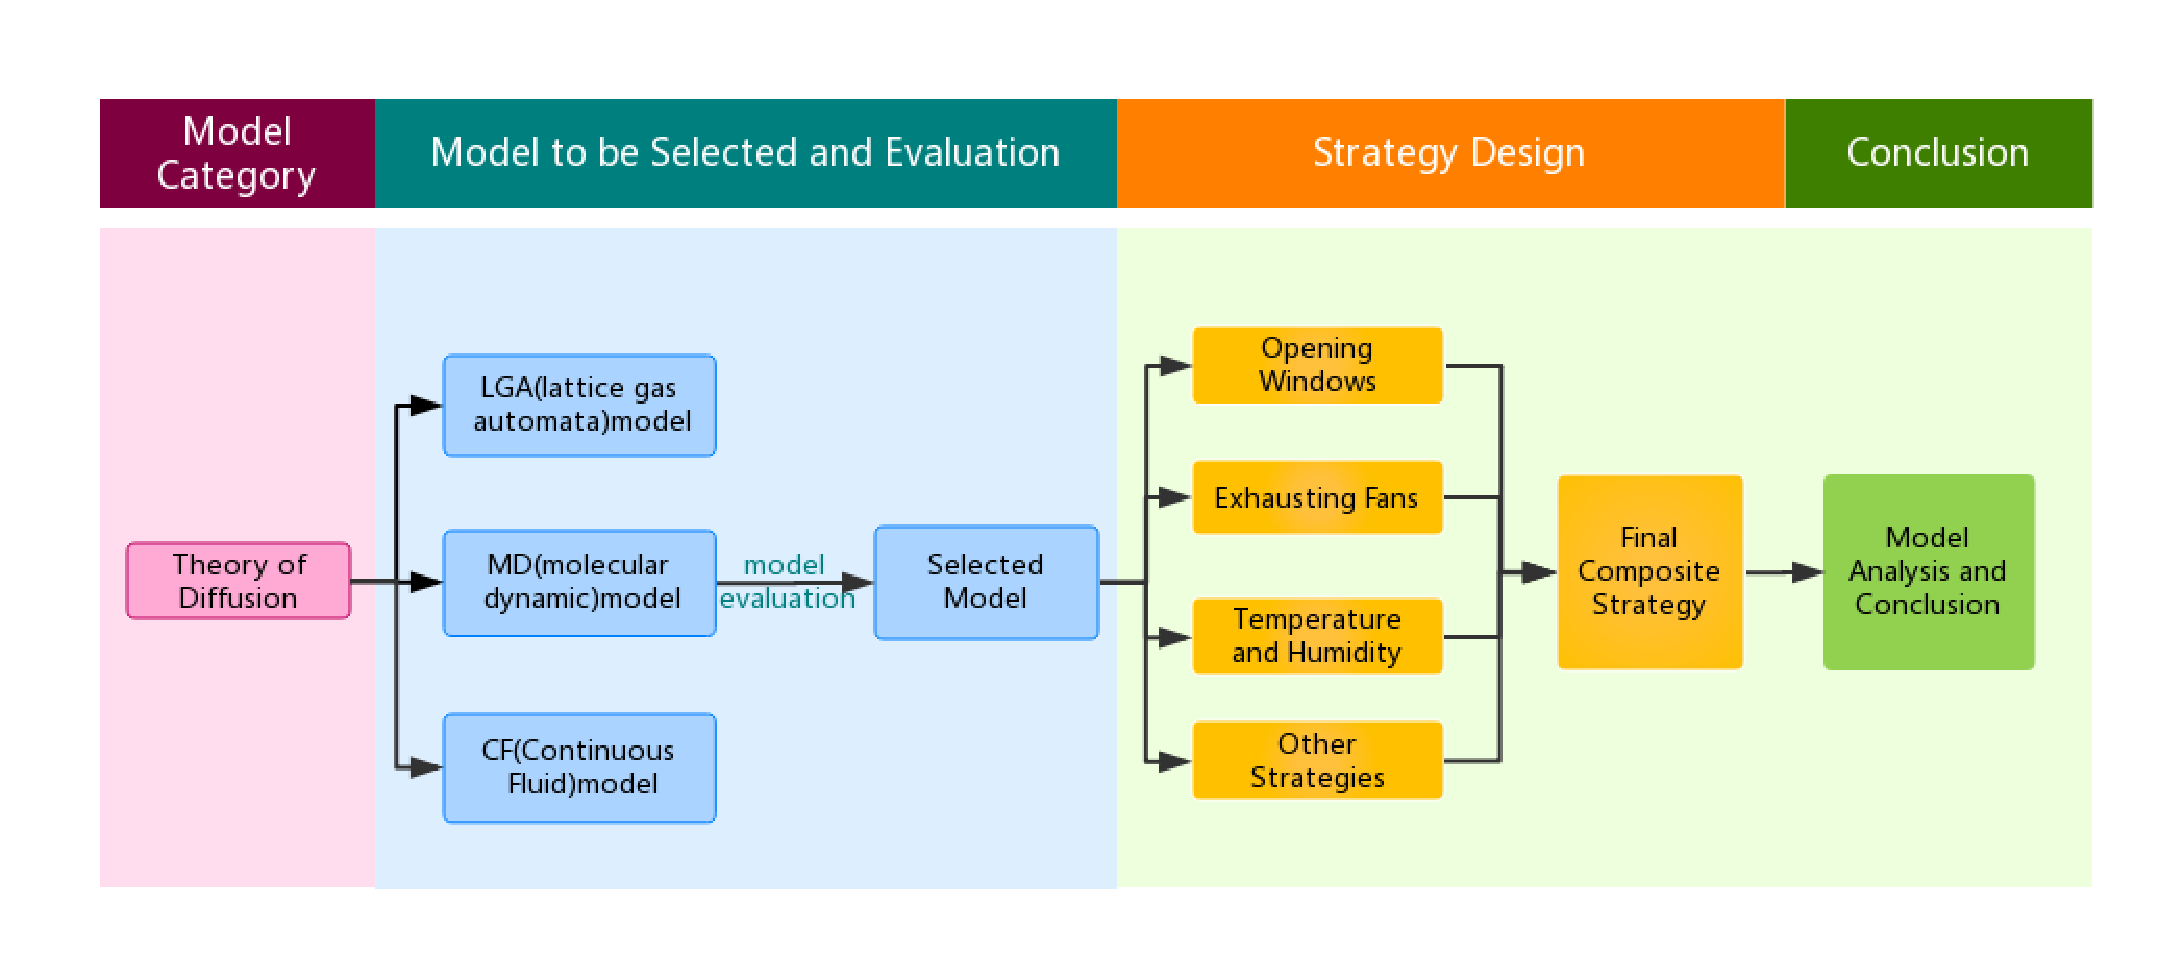
\includegraphics[width=\textwidth]{model.pdf}
  \caption{Framework of Our Work}
  \label{fig:Frame}
\end{figure}

\section{Assumptions and Notations}
\subsection{Assumptions}
We derived three models and they make the following assumptions in common.
\begin{enumerate}
	\item Without loss of generality, we consider our room a cube because almost every apartment in reality consists of a few cubes or cuboids. Meanwhile, the discussion on cube room can be easily generalized to cuboid room. The effect of interior walls will be discussed in an individual section.
    \item The thickness of the wall can be ignored so that the volume of the room equals the capacity of the room.
    \item In our basic models, rooms are closed all around with its interior containing only formaldehyde gas.
    \item The formaldehyde gas is uniformly distributed in every wall except the floor and can only be released inward.
   \item There's no gas exchange between the house and the outside unless the window is open or the exhausting fans are applied, which will be discussed as additional strategies later.
   
\end{enumerate}


\subsection{Notations}

\begin{table}[H]
  \begin{center}
    \caption{Notations.}
    \label{tab:Not}
    \begin{tabular}{ccc}
      \toprule
      Symbol & Definition & Unit\\
      \midrule
      $W$ & Width of a house & m\\
      $L$ & Length of a house & m\\
      $H$ & Height of a house & m\\
      $\sigma$ & Formaldehyde gas particles contained in the wall per unit area & m$^3$\\
      $\Delta \tau$ & the time per frame for the simulation of LGA model & s\\
      $\overline \rho $ & Average density of formaldehyde gas in house & m$^{-3}$\\
      $\rho_{threshold}$ & Threshold density of formaldehyde gas & m$^{-3}$\\
      $J$ & Diffusion flux & mol$\cdot$m$^{-2}$s$^{-1}$\\
      $D$ & Diffusion coefficient & m$^2$/s\\
      $\varphi(\vec{x},t)$ & Molar concentration in position $\vec{x}$ and time t& mol$\cdot$m$^{-3}$\\
      $t_{threshold}$ & Time needed to decline to health threshold & d\\
      \bottomrule
    \end{tabular}
  \end{center}
\end{table}

\section{Model Construction and Implementation}
\subsection{Theory of Diffusion}
Diffusion is the net movement of molecules or atoms from a region of high concentration with high chemical potential to a region of low concentration with low chemical potential. The rate of diffusion, which is quantified by diffusion flux, the rate of flow of amount of substance per unit area is proportional to the concentration gradient. This is described by Fick's First Law as following.
\begin{equation}
J=-D\nabla\varphi
\end{equation}
This law has told us that the concentration gradient is the driving force of transport phenomena, but what we care most is the evolution of concentration with time. This is given by Fick's Second Law.

First, use mass conservation law
\begin{equation}
\frac{\partial\varphi}{\partial t}+\nabla J=0
\end{equation}
Then Fick's first law is applied,
\begin{equation}
\frac{\partial\varphi}{\partial t}=\nabla(D\nabla\varphi)=D\Delta\varphi
\end{equation}

What we need to do next is set all the boundary conditions and solve the partial equation above to get distribution function $\varphi(\vec{x},t)$, which will offer us all the preferred physical quantity such as the minimum time which concentration falls below threshold, the concentration of formaldehyde gas in a place of interest at a given time.


\subsection{Lattice Gas Automata(LGA) Model}

We start with Lattice Gas Automata model, a rough model which is enough to help us understand the behavior of diffusion of formaldehyde gas. This model treat real gas as lattice gas and makes the following additional assumptions:
\begin{enumerate}

\item We consider the room as a lattice, and the formaldehyde gas as a gas unit point regardless of its shape or intrinsic properties.

\item Evolution of the simulation is done in discrete time steps. After each time step, the state at a given site can be determined by the state of the site itself and neighboring sites, before the time step.

\item The state at each site is purely boolean. At a given site, there either is or is not a unit gas moving in each direction.

\item The effect of air is ignored, since compared with formaldehyde, the concentration of air is too large to matter on the behavior of flow of formaldehyde gas. Although the average velocity, escape time can be totally different in vacuum or atmosphere, the parameters of properties of gas unit can be adjusted.


\item The formaldehyde gas generating rate is even over time and space along the wall.

\end{enumerate}

The LGA model was introduced by Hardy, de Passis, and Pomeau in 1976 \cite{PhysRevLett.56.1505} and is also called the HPP model, a name derived from its inventors. Initially used for the description of the molecular dynamics of a classical lattice gas, the LGA was later used to model large numbers of uniformly interacting particles (cells). In our model, LGA are used to simulate the diffusion of formaldehyde.

LGA employs a regular, finite lattice and includes a finite set of particle states, an interaction neighborhood and local rules which determine the movement of particles (cells) and their transitions between states.\cite{weimar1997simulation} LGA differs from traditional CA by incorporating the movement of particles and an exclusion principle. The particles in the model select from a finite number of permissible discrete velocity channels. The velocity specifies the direction and magnitude of movement, which may include zero velocity (rest). In a simple exclusion rule, only one particle may have each allowed velocity at each lattice site.

According to the dimensions, LGA model can be divided into 2 categories:2D and 3D\cite{3D_model}. Every node in the 2D LGA model is associated with five velocity channels, namely stay, left, right, up, and down. Similarly, each node in a 3D LGA model has seven velocity channels associated with it-stay, left, right, up, down, front, and back. For the case of a 2D LGA model, the number of velocities and their possible directions are shown in Fig1.

\begin{figure}[H]
  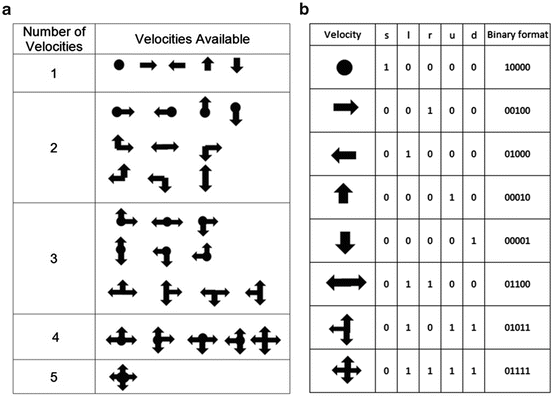
\includegraphics[width=\linewidth]{LGA.png}
  \caption{(a) The number of velocities available in a node and their possible directions for a 2D LGA. (b) Examples of binary representation of some possible velocities at a node in a 2D LGA}
  \label{fig:LGA_state}
\end{figure}

In our model, the density of formaldehyde follows the formula:

\begin{equation}
 WLH\frac{{d\overline \rho  }}{{dt}} = \sigma [2H(W + L) + WL]
\end{equation}
where $\sigma$ is not a constant because of the emission of formaldehyde. To simplify the process of simulation of our modeling, we ignore the emission from the ceiling so the density of formaldehyde follows:
\begin{equation}
 WLH\frac{{d\overline \rho  }}{{dt}} =2\sigma H(W+L)
\end{equation}
as there is no emission from ceiling and floor and in order to give a better intuition, we first run our LGA in 2-dimension scene using C++.

  In the simulation, the house are set to be $5($L$)\times3($W$)\times3.5($H$)$ ,so we draw $1500\times900$ lattices to represent the cross section of the house. In the beginning there is no formaldehyde particles in the air ,they are only stored in the walls. The yellow dot in \ref{fig:simu} represents the formaldehyde particles, it's clear that formaldehyde cluster near the wall and it's density takes the minimum in the center of the house's cross section.
  
\begin{figure}[H]
  \centering
  \begin{subfigure}[b]{0.48\linewidth}
    
\includegraphics[width=\linewidth]{0.png}
    \caption{$t$=0}
  \end{subfigure}
  \begin{subfigure}[b]{0.48\linewidth}
    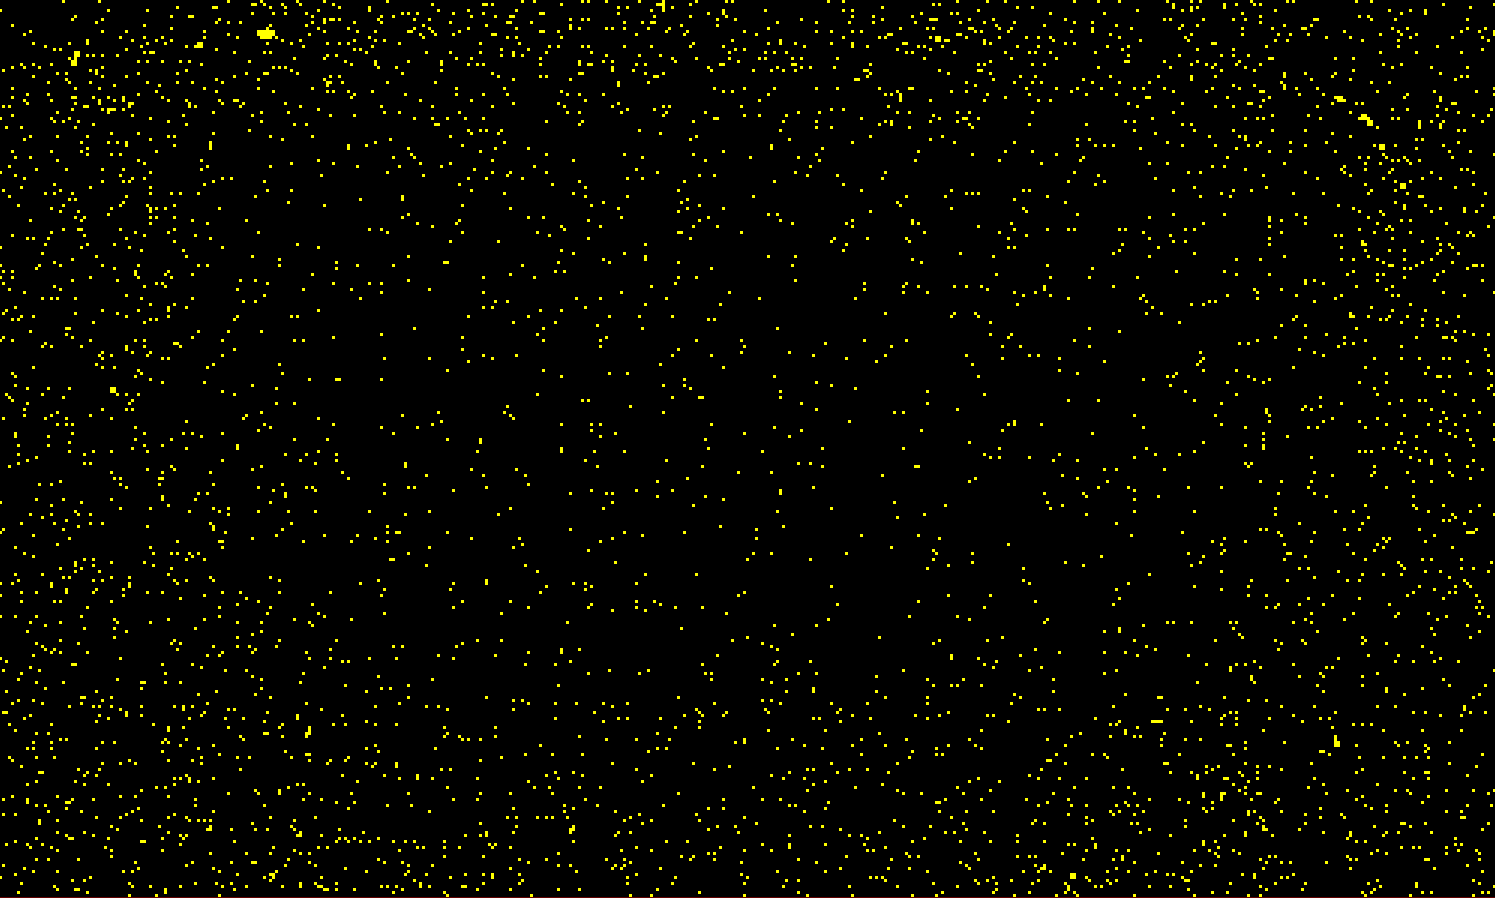
\includegraphics[width=\linewidth]{500.png}
    \caption{$t$=500$\Delta \tau$}
  \end{subfigure}\\
  \begin{subfigure}[b]{0.48\linewidth}
    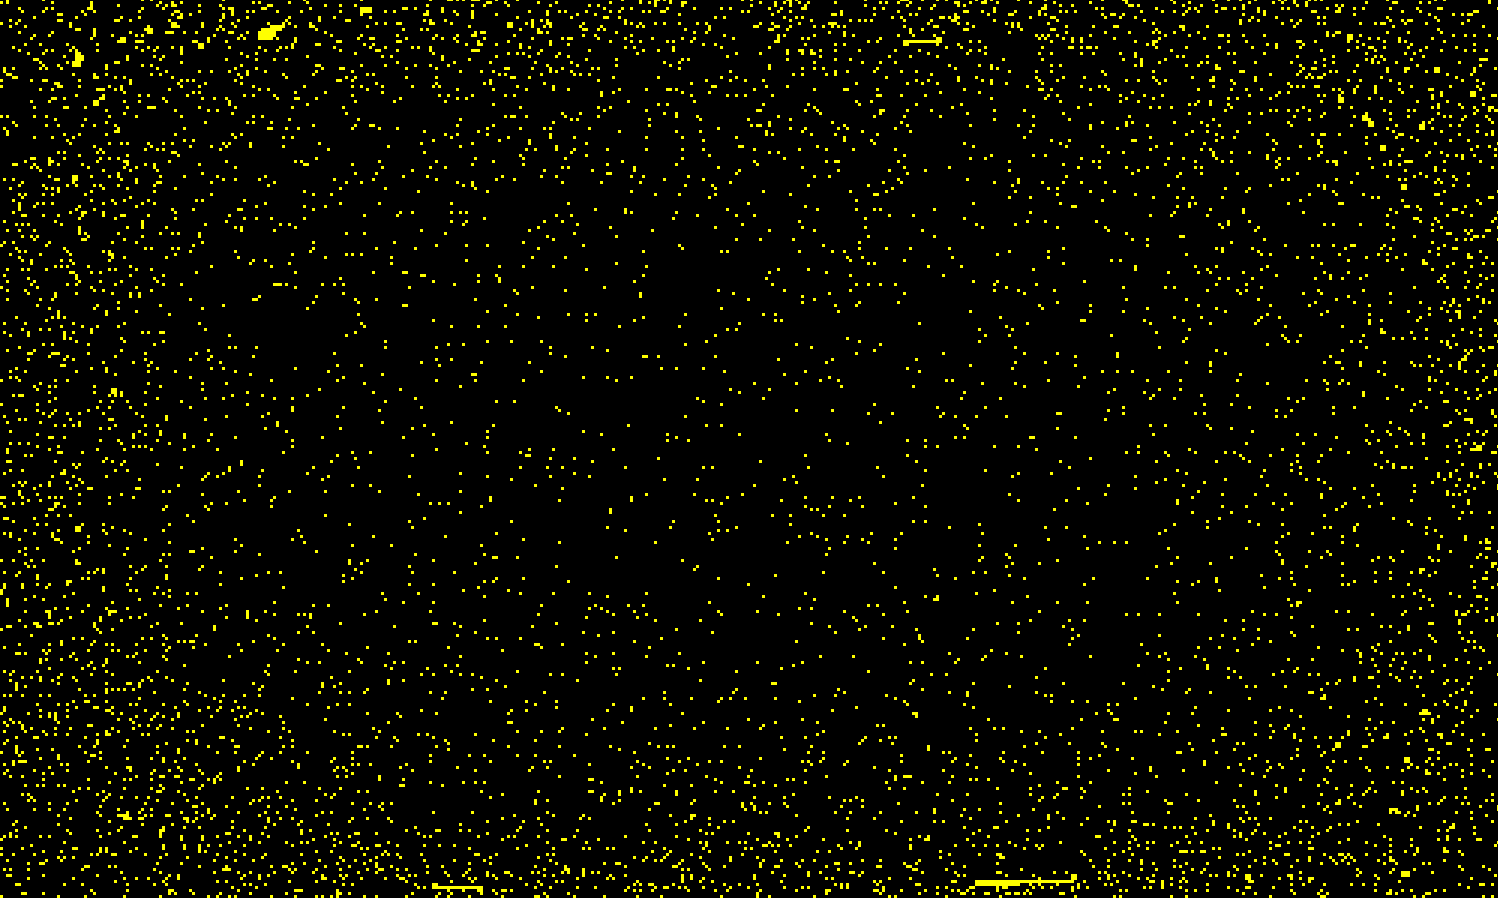
\includegraphics[width=\linewidth]{1000.png}
    \caption{$t$=1000$\Delta \tau$}
  \end{subfigure}
  \begin{subfigure}[b]{0.48\linewidth}
    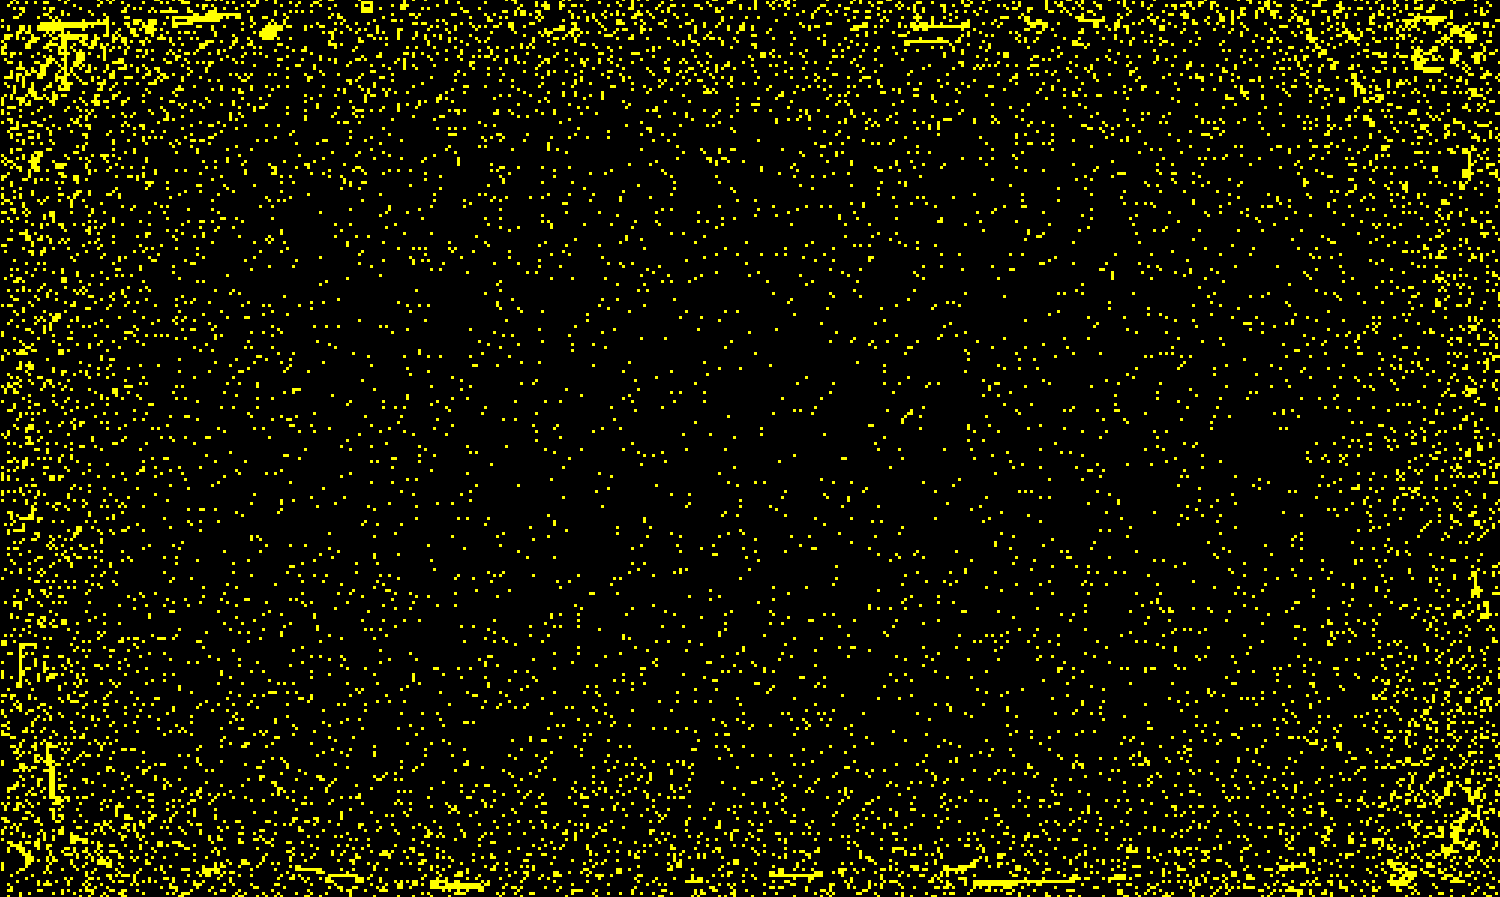
\includegraphics[width=\linewidth]{2000.png}
    \caption{$t$=2000$\Delta \tau$}
  \end{subfigure}
  \caption{Simulation of the LGA model using C++}
  \label{fig:simu}
\end{figure}
  
\subsection{Molecular Dynamics(MD) Model}
Despite the rough LGA model mentioned above,we now try to be more specific by simulating the diffusion of particles following the rules of classical mechanics.Therefore, we introduce the additional assumptions as follows:
\begin{enumerate}

\item We use a simple sphere to represent a molecule of formaldehyde and take the strategy of coarse-grained modelling.By decreasing the degrees of freedom much longer simulation times can be studied than using classical atomistic models. 

\item The interactions between the particles strictly abide by the Newton's second law of mechanics and Momentum conservation law.

\item Since the concentration of the air is at a much higher scale than formaldehyde, the behavior of diffusion of formaldehyde has no much difference to the particles in vacuum except velocity which can be modified by adjusting parameters.

\end{enumerate}

To improve computational accuracy, we tackle this molecular dynamic problem using Verlet integration method \cite{paterlini1998constant}, which is a numerical method used to integrate Newton's equations of motion.
At first ,we define:$v(t+\Delta t/2)\equiv (x(t+\Delta t)-x(t))/\Delta t$

It is obvious that:
$x(t+\Delta t)\approx 2x(t)-x(t-\Delta t)+\dfrac{F(x_i)}{m} \Delta t$

so we can get  $x(t+\Delta t/2)=x(t)+\Delta t v(t+\Delta t/2)$

Because of this, the equations for updating position and velocity are:
\begin{equation}
x_i=x_{i-1}+v_{i-1/2}\Delta t
\end{equation}
\begin{equation}
a_i=F(x_i)
\end{equation}
\begin{equation}
v_{i+1/2}=v_{i-1/2}+a_i \Delta t
\end{equation}
where $x_{i}$is position at step $i$, $v_{i+1/2}$ is the velocity, or first derivative of $x$, at step $i+1/2$, $a_{i}$ is the acceleration, or second derivative of $x$, at step $i$, and $\Delta t$ is the size of each time step. 

Note that the potential for particles should be set individually, we choose use Lennard-Jones potential\cite{lennard1931cohesion} to do our simulation, which is widely used in molecular dynamics and really resembles the real condition.

\subsection{Continuous Fluid(CF) Model}

In physics and engineering, fluid dynamics is a sub-disciplines of fluid mechanics that describes the flow of fluids (liquids and gases). Fluid dynamics has a wide range of applications, including calculating forces and moments on aircraft, determining the mass flow rate of petroleum through pipelines, predicting weather patterns and so on. In our model, the flow of formaldehyde can be viewed as continuous fluid rather than discrete particles. We derive Continuous Fluid(CF) model from it, the fluid of formaldehyde follows the conservation laws' equation:
\begin{equation}
\frac{\partial}{\partial t}\iiint _{V}\rho \,dV=-\,\oiint _S \,\rho\mathbf {u}\cdot d\mathbf{S}
\end{equation}
\begin{equation}
{\frac {\partial }{\partial t}}\iiint _{\scriptstyle V}\rho \mathbf {u} \,dV=-\,{} \oiint _{\displaystyle _{\scriptstyle S}} {\displaystyle (\rho \mathbf {u} \cdot d\mathbf {S} )\mathbf {u} -{}}-{} \oiint_{\displaystyle {\scriptstyle S}} \,p\,d\mathbf {S}  {\displaystyle \displaystyle {}+\iiint _{\scriptstyle V}\rho \mathbf {f} _{\text{body}}\,dV+\mathbf {F} _{\text{surf}}}
\end{equation}
\begin{equation}
\rho \frac{Dh}{Dt}=\frac{Dp}{Dt}+\nabla\cdot\left(k\nabla T\right)+\Phi 
\end{equation}

Based on the conservation laws' equation of fluid and the Fick's first law we have discussed before, we can derive Fick's second law:
\begin{equation}
\frac{\partial}{\partial x}\left(\,D\,{\frac {\partial }{\partial x}}\varphi \,\right)=D\,{\frac {\partial }{\partial x}}{\frac {\partial }{\partial x}}\,\varphi =D\,{\frac {\partial ^{2}\varphi }{\partial x^{2}}}
\end{equation}

Then we are discussing constants needed and all boundary conditions that are necessary to numerically solve the partial differential equation.
\begin{itemize}
	\item The diffusion coefficient of formaldehyde $D$ = $1.8\times 10^{-5}$m$^2/$s in air, according to GSI Database\footnote{https://www.gsi-net.com/en/publications/gsi-chemical-database/single/288-CAS-50000.html}.
	\item The concentration on the surface of the wall are given by the assumption that formaldehyde is uniformly distributed initially, and then evolves according to Fick's law.
    \item As for windows taken into consideration later, that treating the concentration along the window as $0$ is enough to simulate the real-life window.
\end{itemize}
Solving this differential equations, we'll get the solution and the characterization concentration of formaldehyde, namely, $\varphi$. As we assume that the air in the house to be the homogeneous isotropic media, finite element method can be applied to the calculation in the house. We divide the house into large quantity of finite element and apply Fick's Law to it. The result of our calculation is visualized through COMSOL software, the results are shown in \ref{fig:CF}.

\begin{figure}[H]
  \centering
  \begin{subfigure}[b]{0.48\linewidth}
    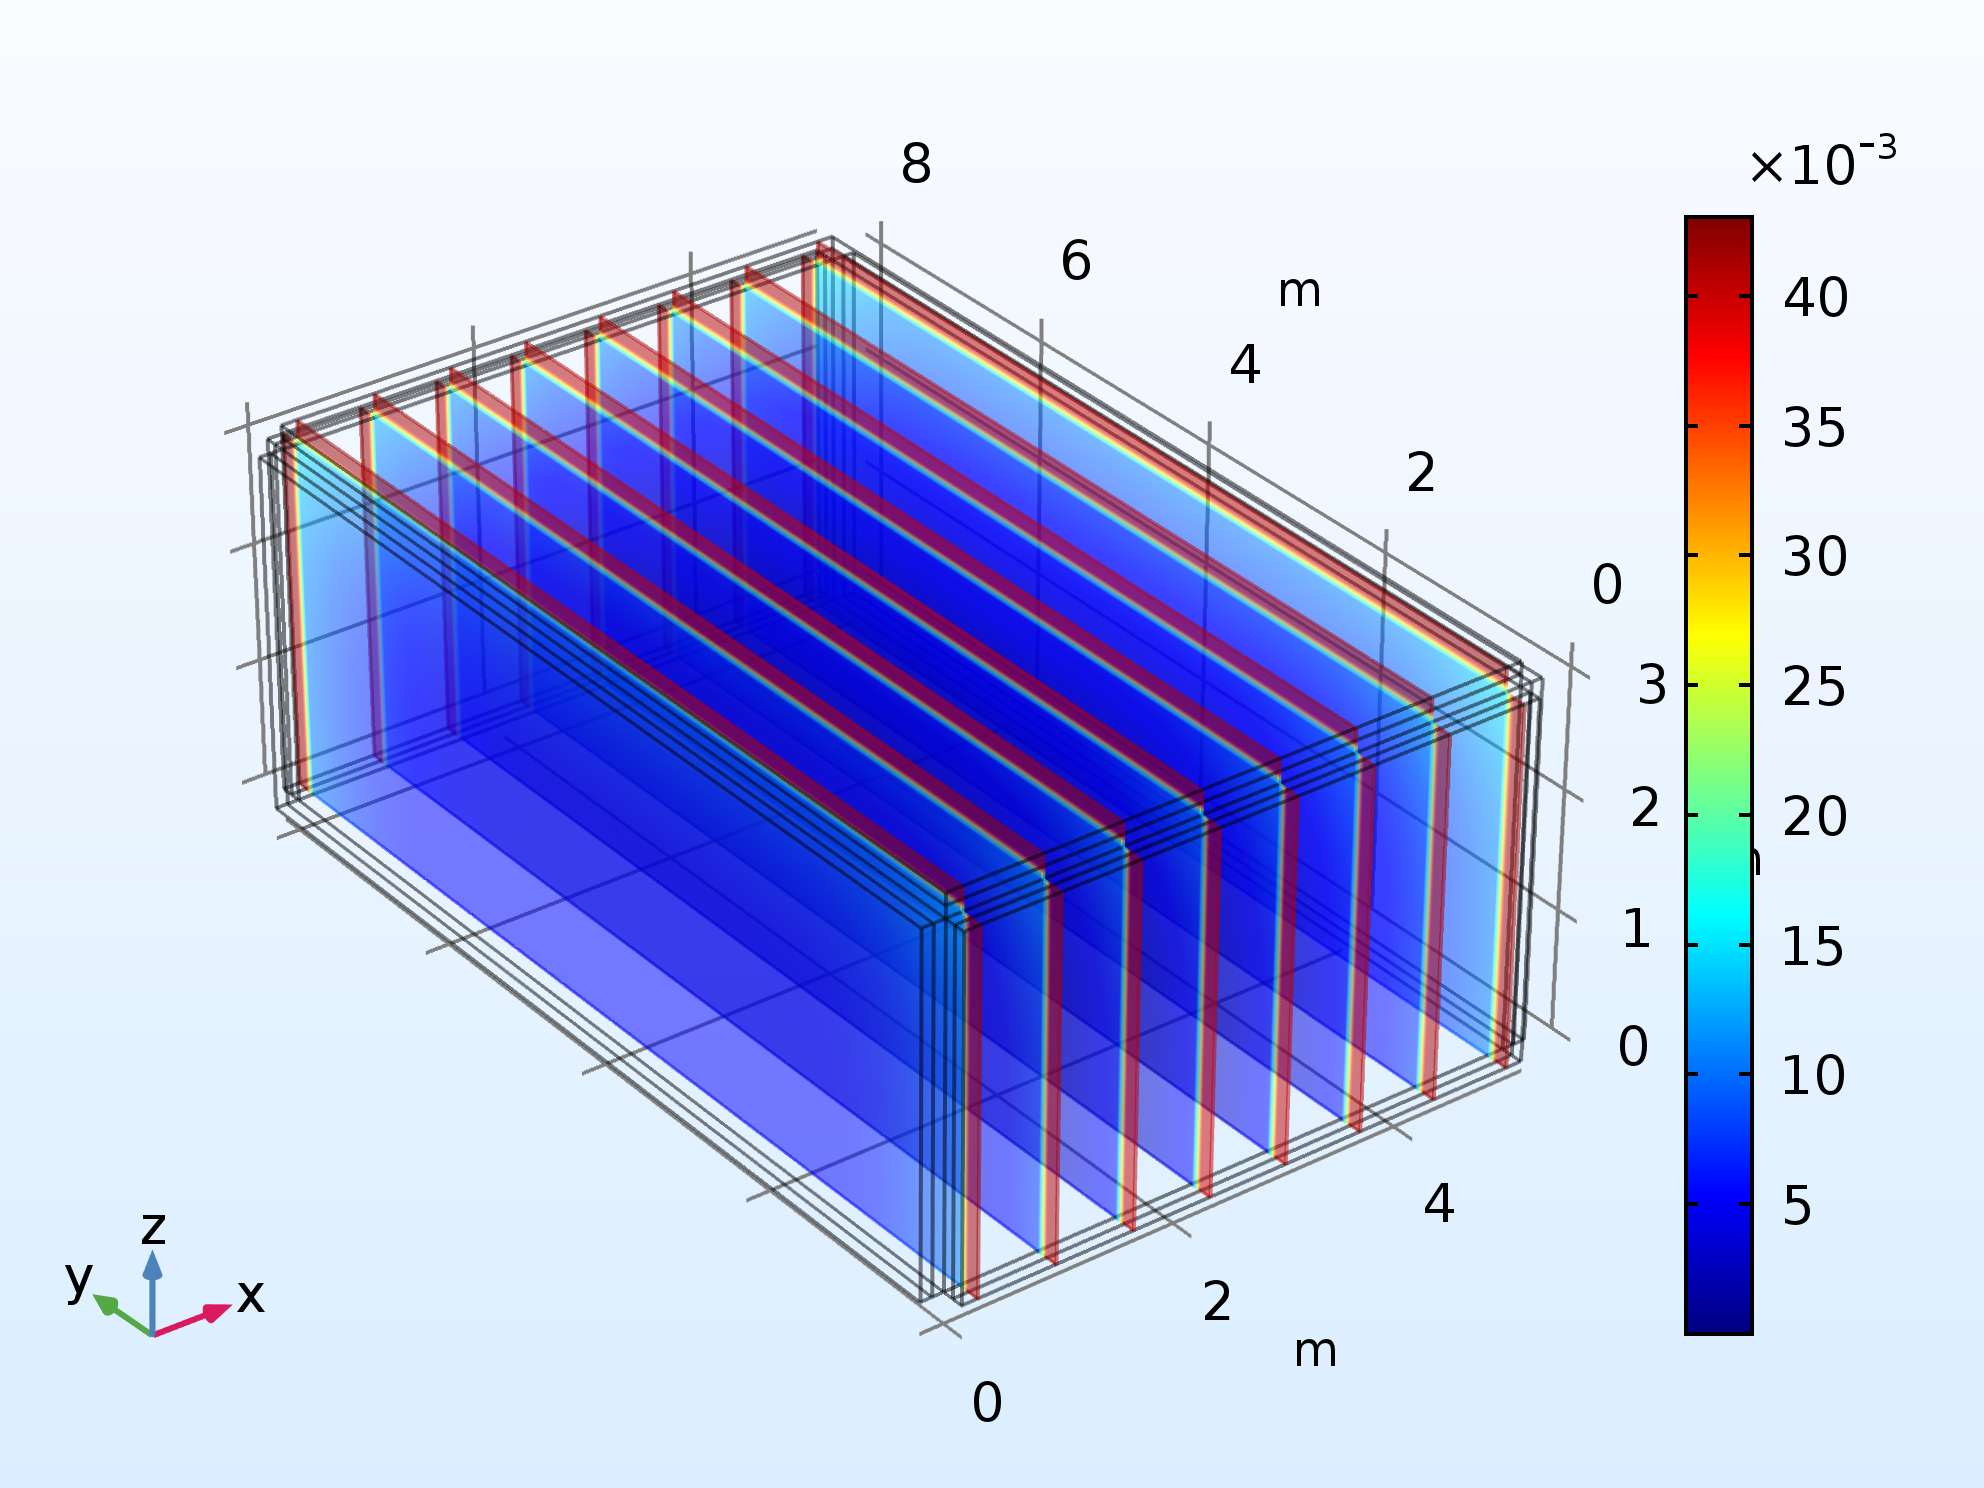
\includegraphics[width=\linewidth]{6h.png}
    \caption{$t$=6$h$}
  \end{subfigure}
  \begin{subfigure}[b]{0.48\linewidth}
    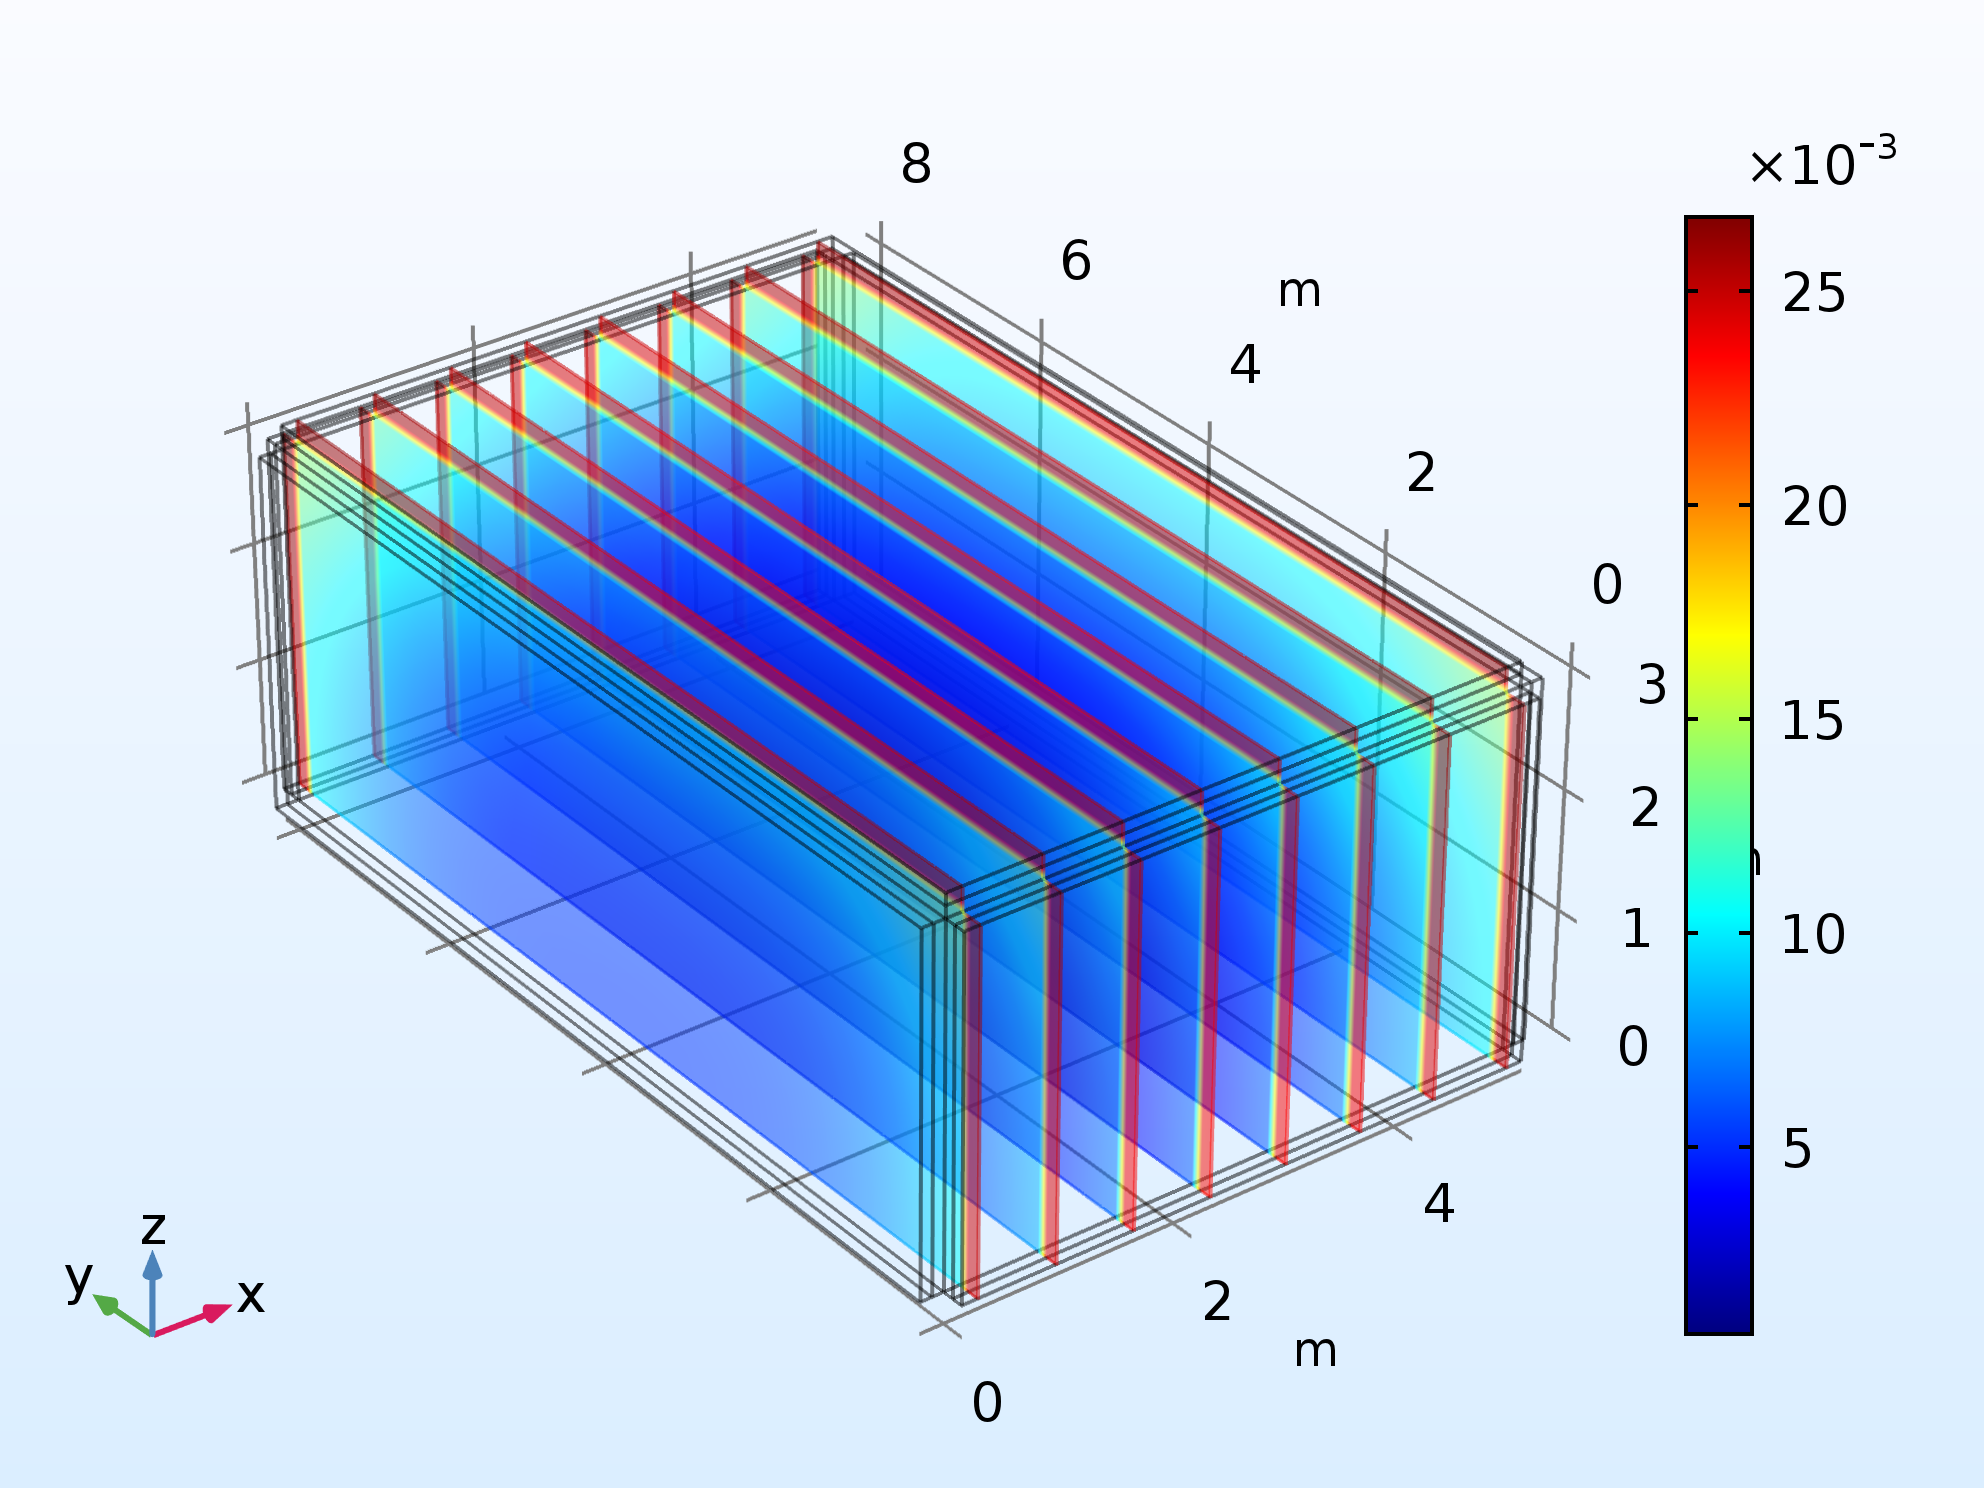
\includegraphics[width=\linewidth]{12h.png}
    \caption{$t$=12$h$}
  \end{subfigure}\\
  \begin{subfigure}[b]{0.48\linewidth}
    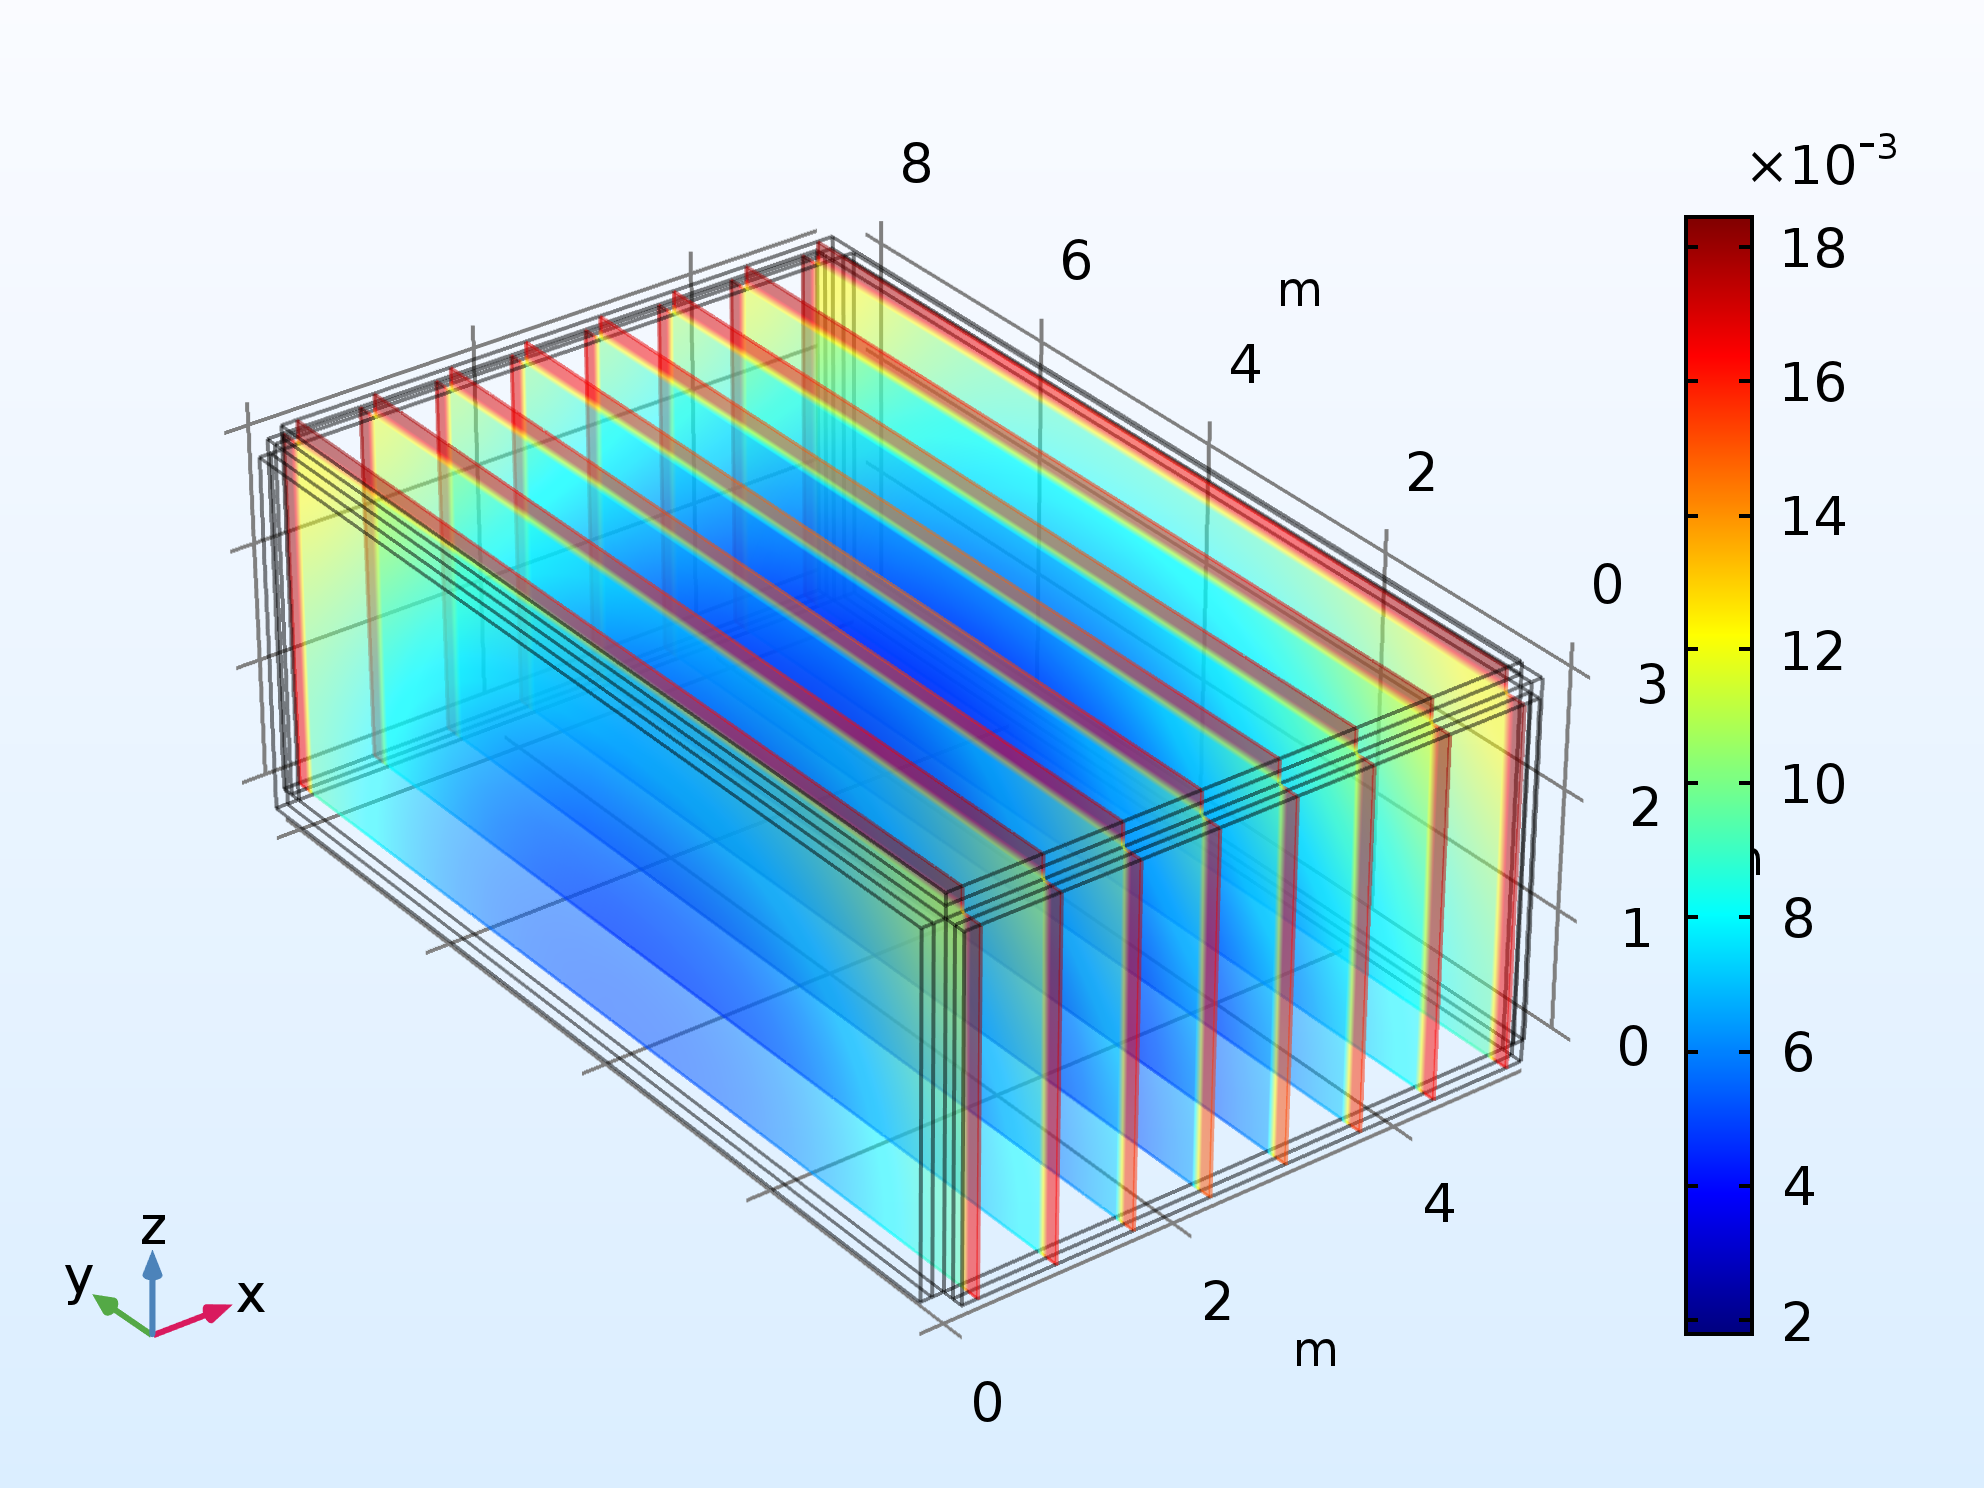
\includegraphics[width=\linewidth]{18h.png}
    \caption{$t$=18$h$}
  \end{subfigure}
  \begin{subfigure}[b]{0.48\linewidth}
    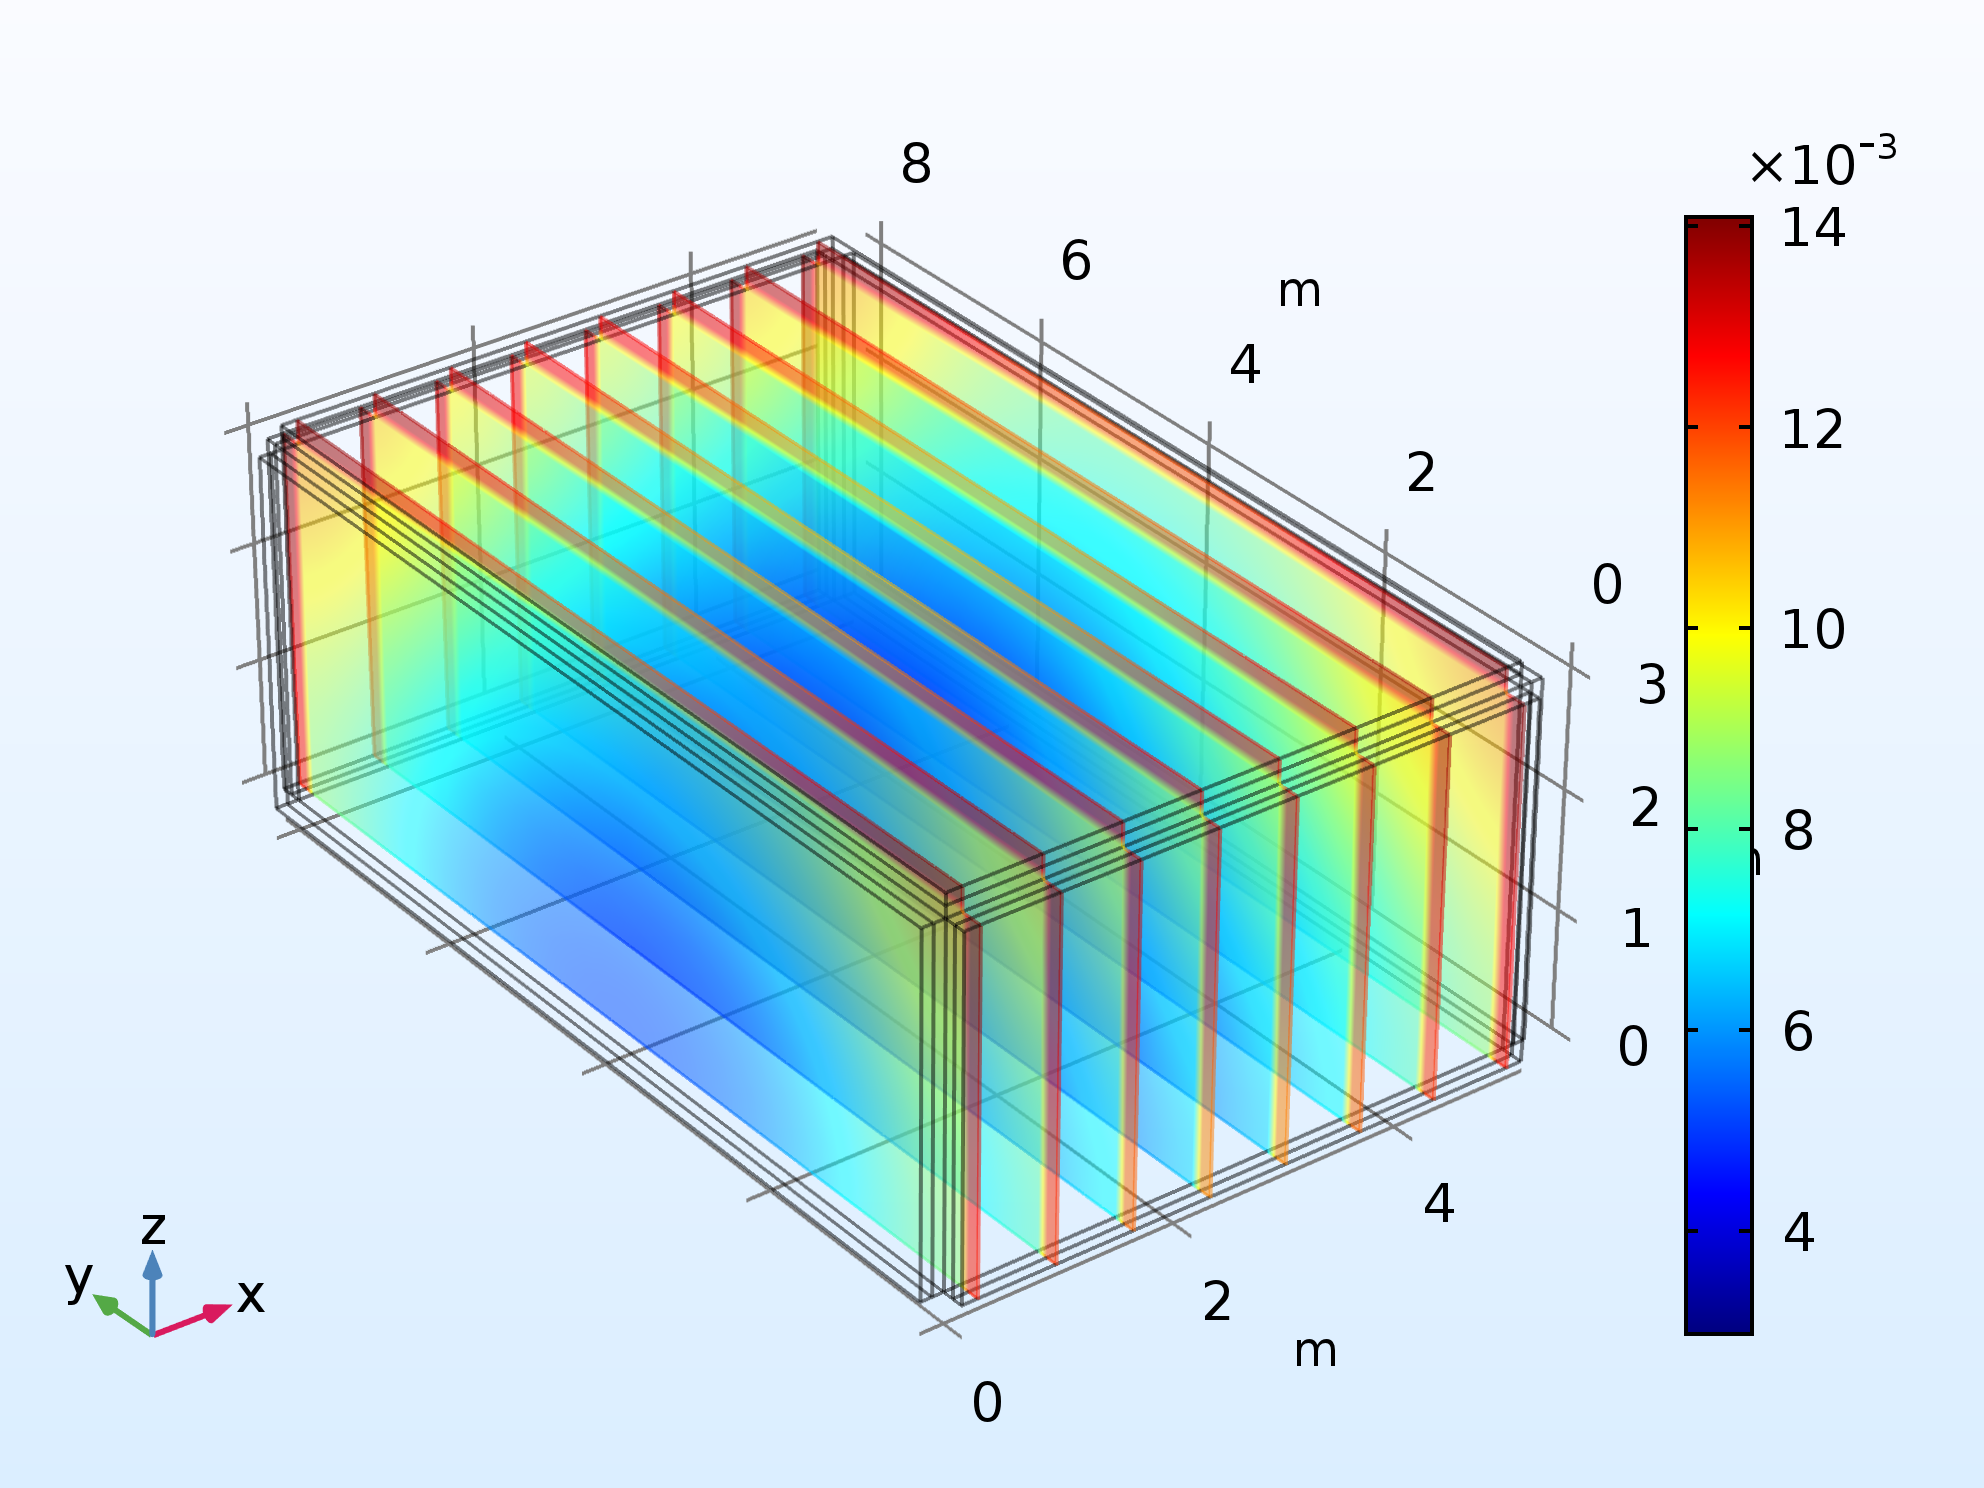
\includegraphics[width=\linewidth]{24h.png}
    \caption{$t$=24$h$}
  \end{subfigure}
  \caption{Simulation of the CF model}
  \label{fig:CF}
\end{figure}

\subsection{Model Analysis and Selection}
Among the model we put forward above, the best model must be selected to continue our work to examine the different strategies. We evaluate our model in terms of accuracy and conciseness.

For accuracy, LGA model makes assumption that the direction of particles' motivation and particles' position is limited, thus leading to inaccuracy of simulation. MD model has better accuracy over LGA model, but it is still difficult to simulate continuous presence of the formaldehyde, because the number of particles is limited by the capability of computation. CF model based on the assumption that the distribution of formaldehyde gas is described by the density function and motion described by Fick's law. To tackle with the partial differential equation, we use finite element method and made a state-of-the-art simulation.

For conciseness, LGA model's assumptions leave out too much information of particles motion and oversimplify the rules of collision. MD model and CF model both reflect the actual motion of particles well as MD model behaves better when the density of formaldehyde is low and CF model behaves better when it's high. In this problem, we know the threshold of concentration which do no harm to people is $3.3\times10^{-6}$mol/m$^3$, which contains still much more number of particles that MD simulation can tackle with.

Taking all these aspects into consideration, we select CF(Continuous Fluid) as our model. Then we'll find and discuss strategies of this model.

\section{Strategies}
\subsection{Opening Windows}

In order to simulate the effect of opening windows, it's necessary to assume that there is no wind outside the window and concentration of formaldehyde gas outside window is $0$. The formaldehyde gas can only diffuse outside through the window. As for the emission source, all the walls and the ceiling are considered storing a certain amount of formaldehyde inside it, which is obtained by data in real life. As for our house, we choose a $8$m(L)$\times 5$m(W)$\times 3$m(H) cuboid house for convenience, the result are shown in Figure \ref{fig:window}


\begin{figure}[H]
  \centering
  \begin{subfigure}[b]{0.3\linewidth}
    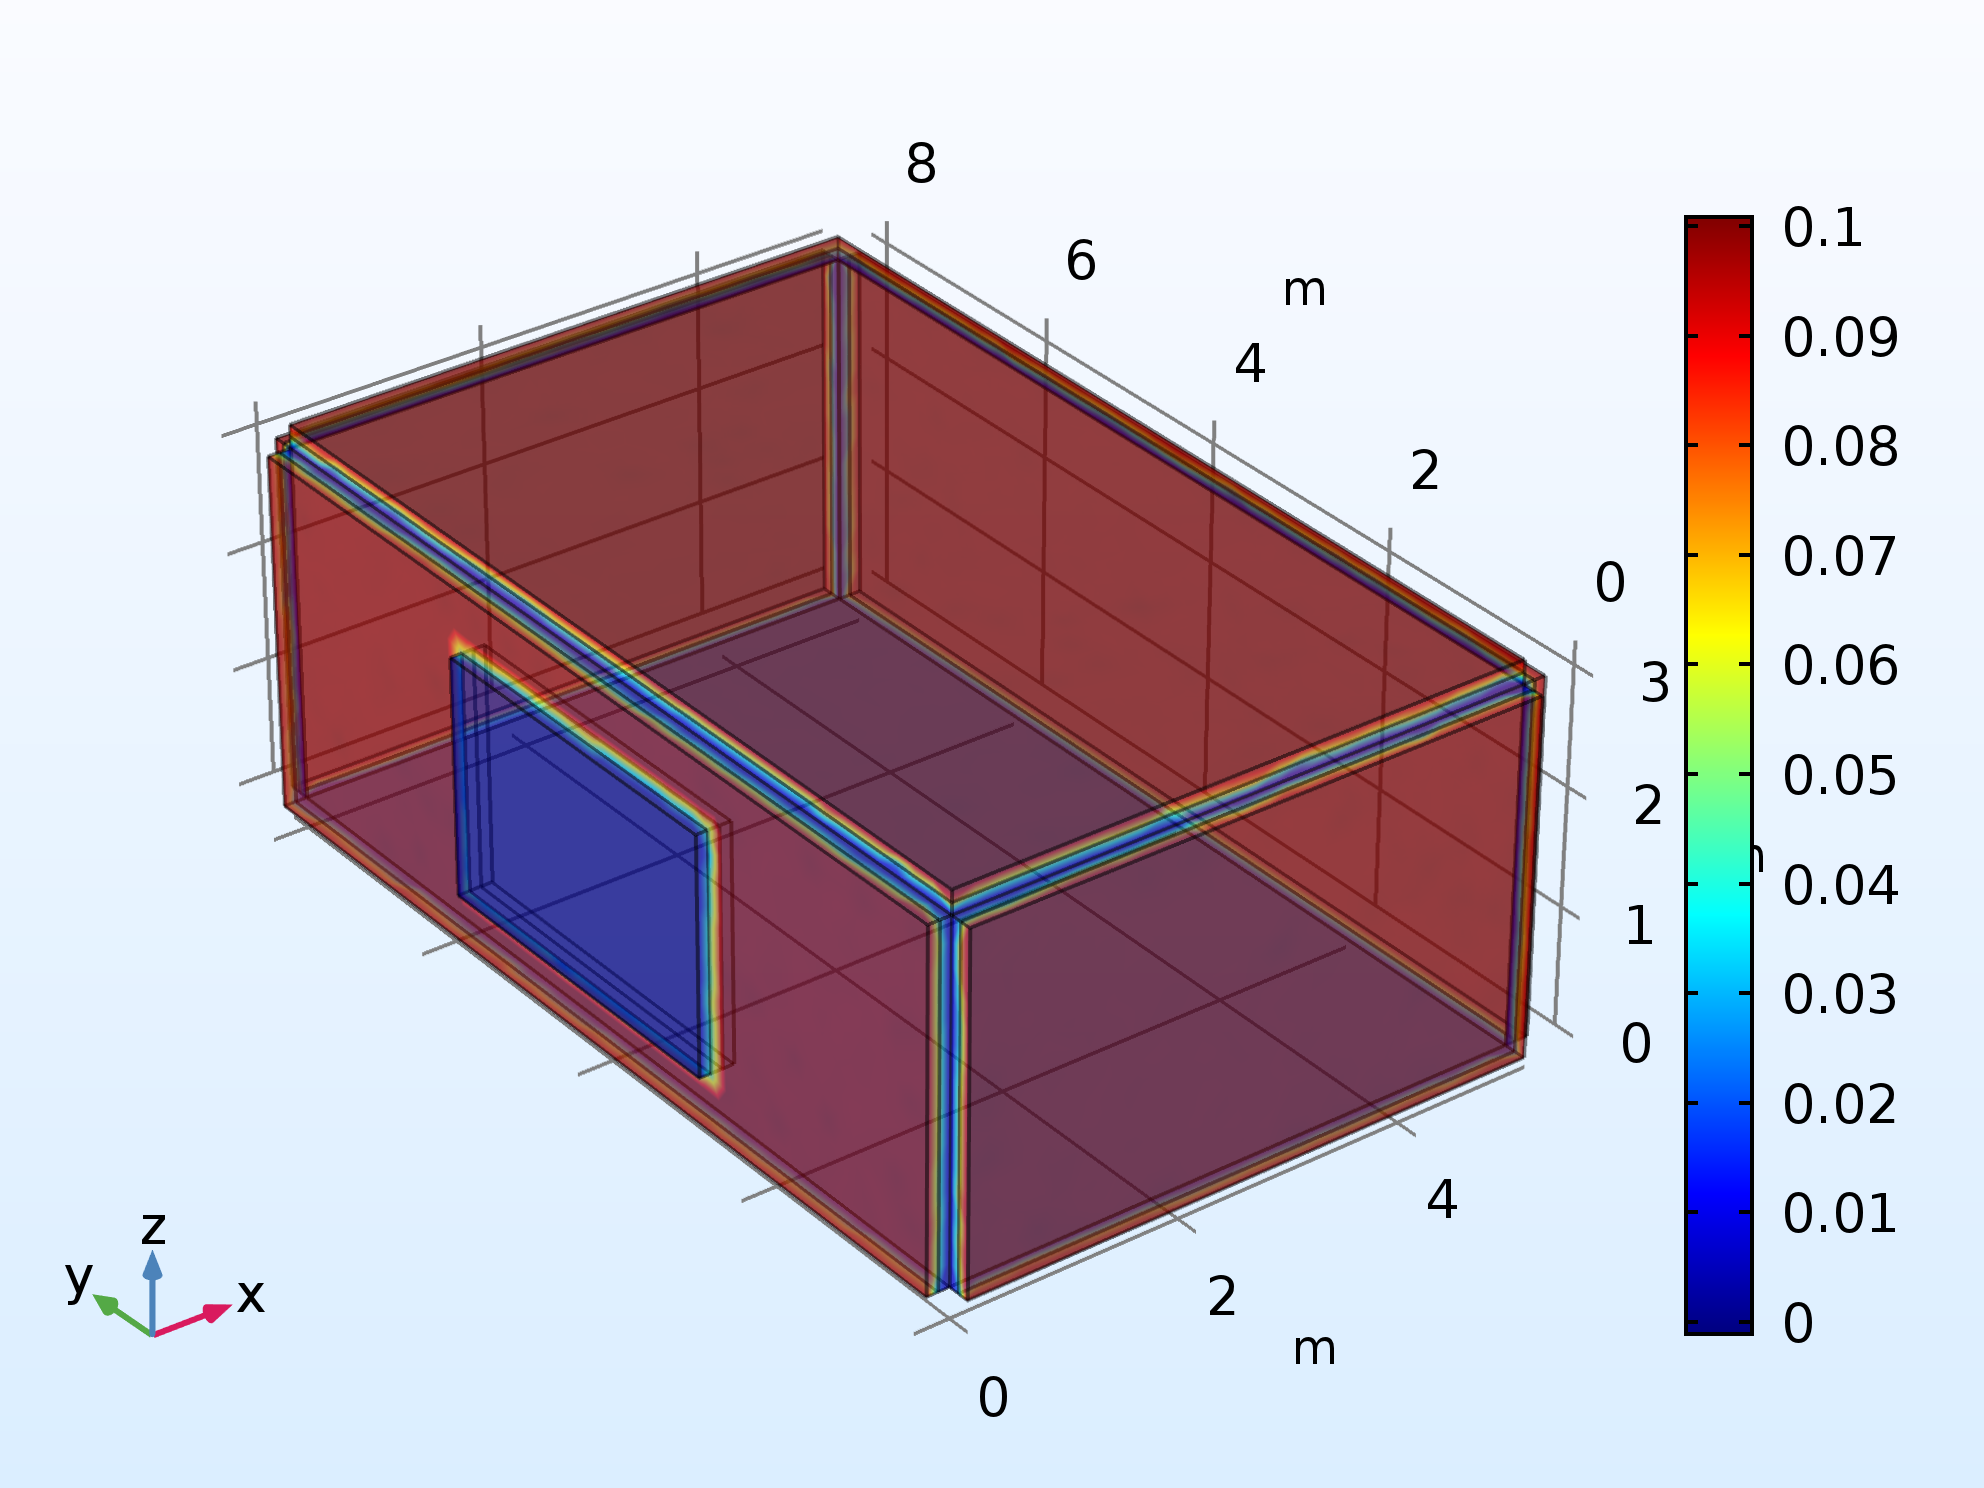
\includegraphics[width=\linewidth]{0d.png}
    \caption{$d$=0}
  \end{subfigure}
  \begin{subfigure}[b]{0.3\linewidth}
    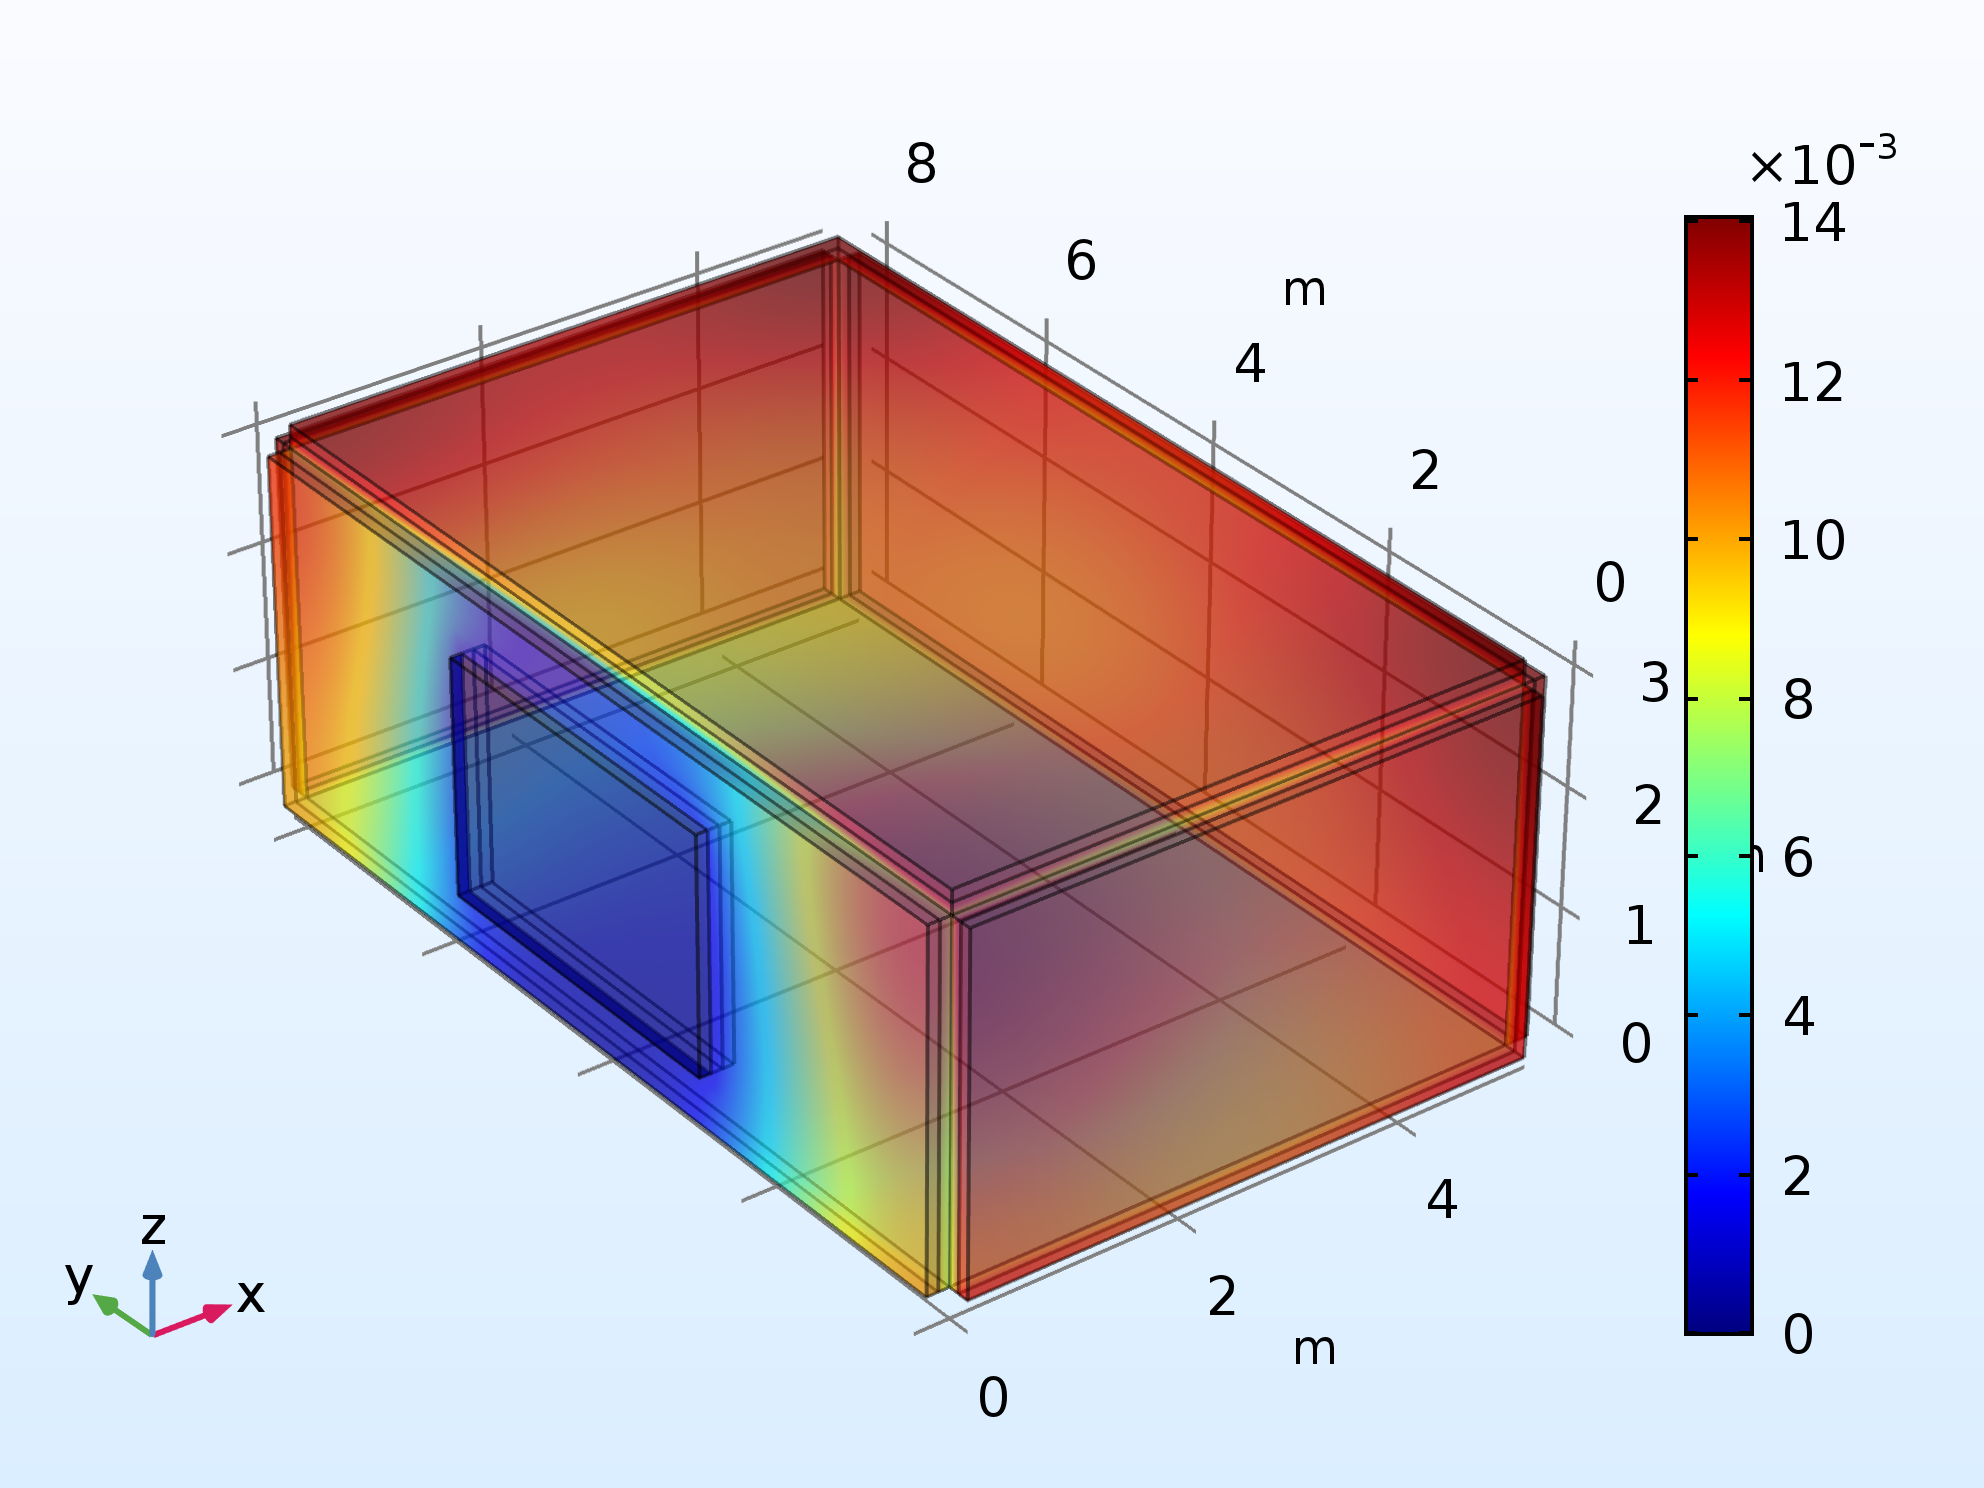
\includegraphics[width=\linewidth]{1d.png}
    \caption{$d$=1}
  \end{subfigure}
  \begin{subfigure}[b]{0.3\linewidth}
    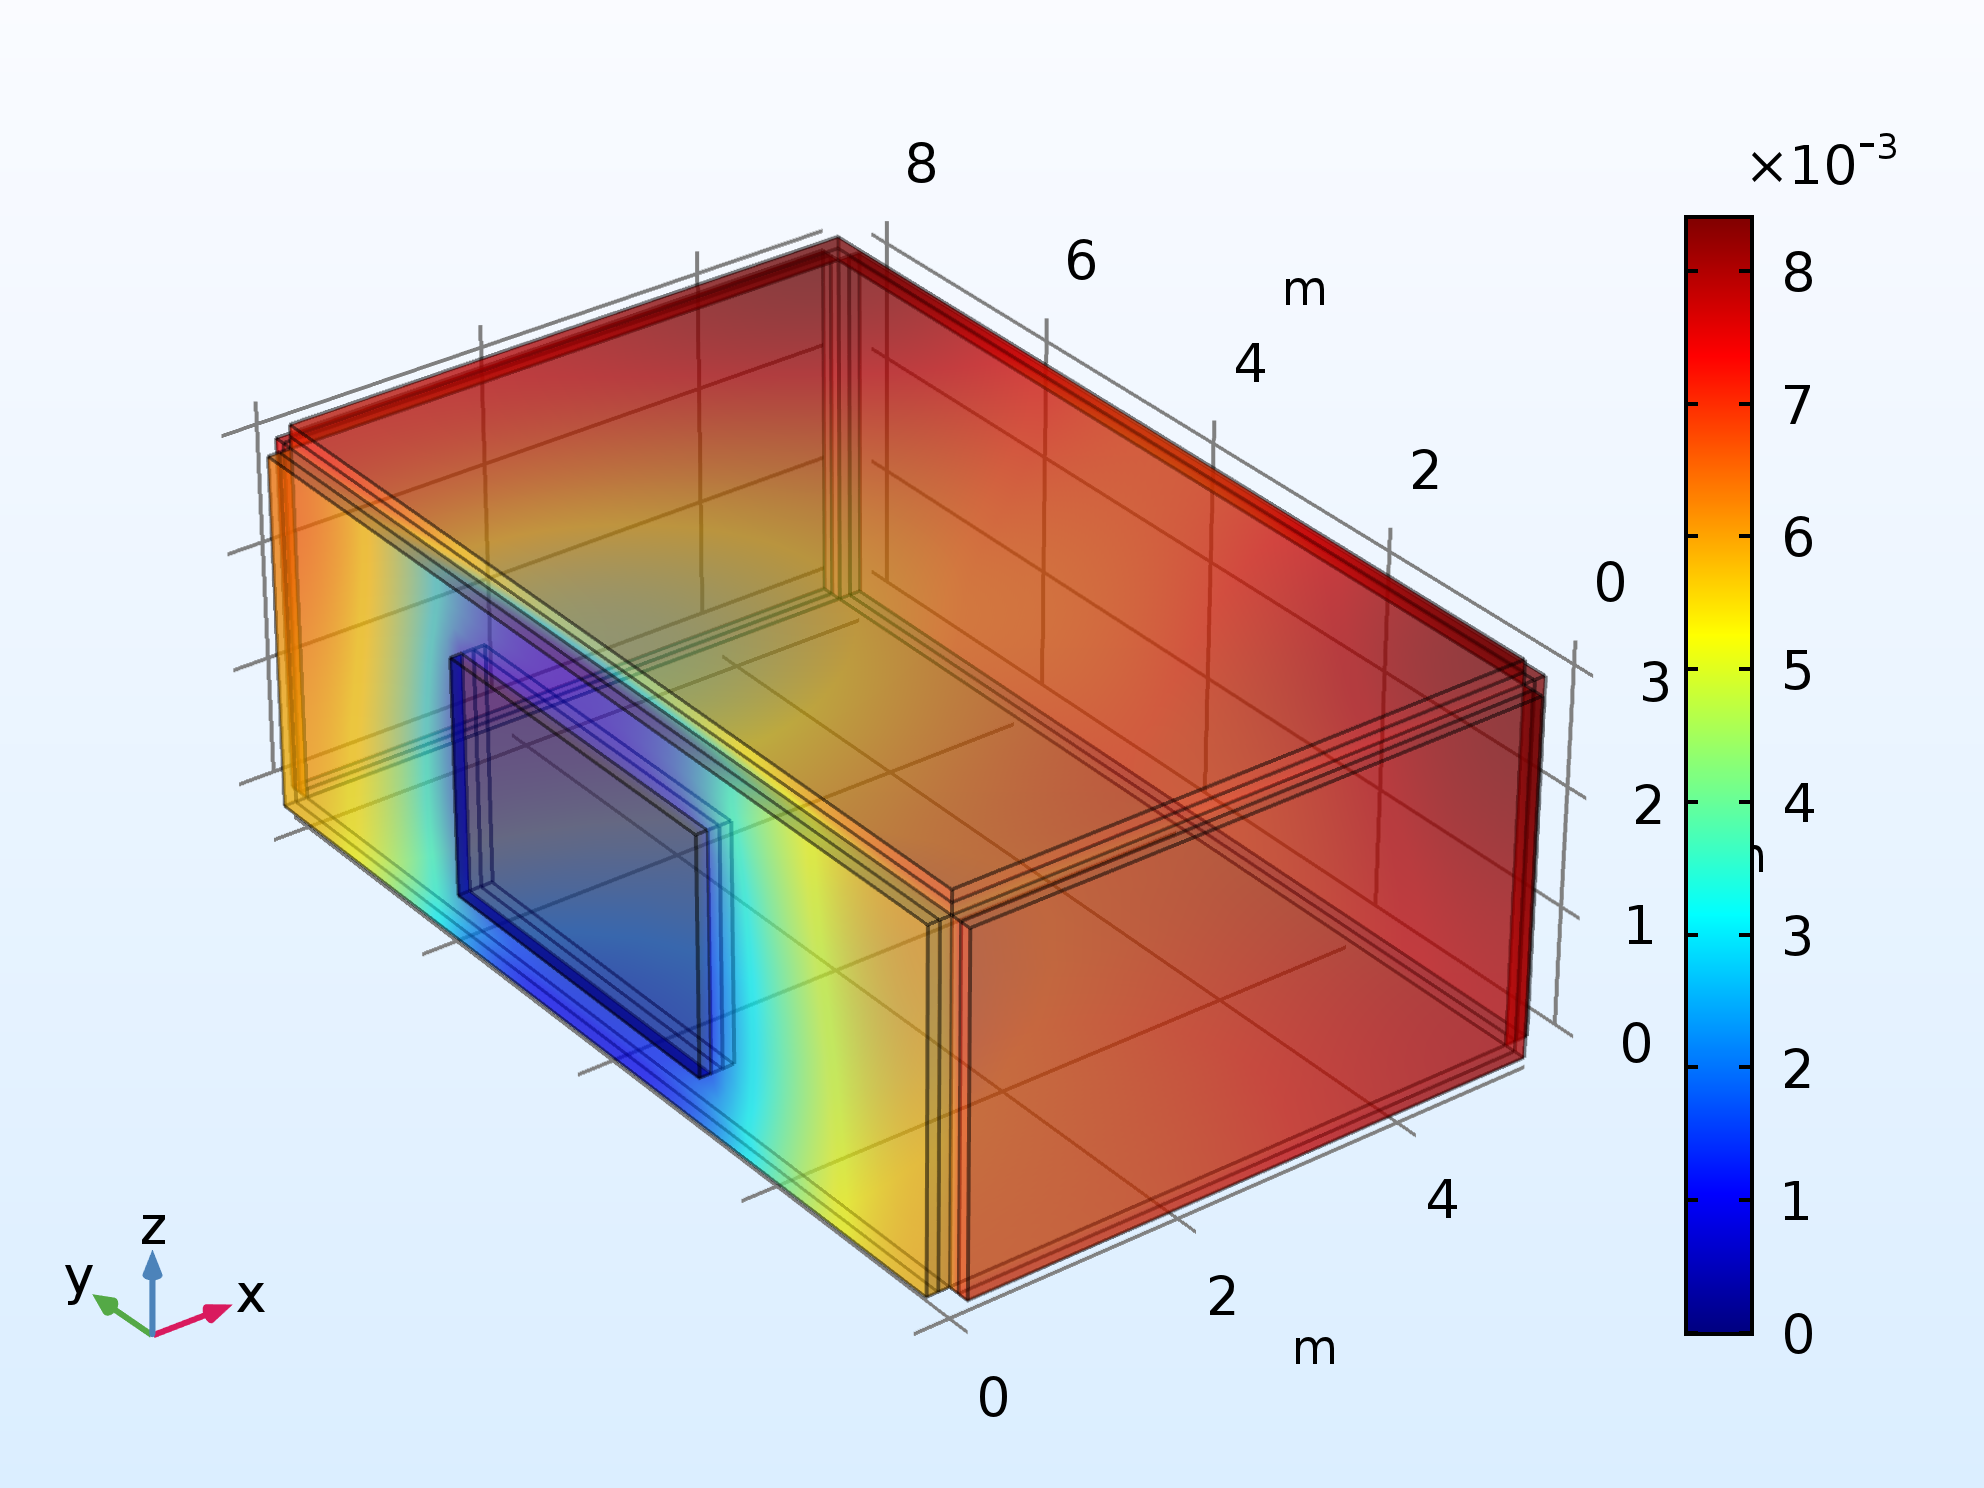
\includegraphics[width=\linewidth]{2d.png}
    \caption{$d$=2}
  \end{subfigure}\\
  \begin{subfigure}[b]{0.3\linewidth}
    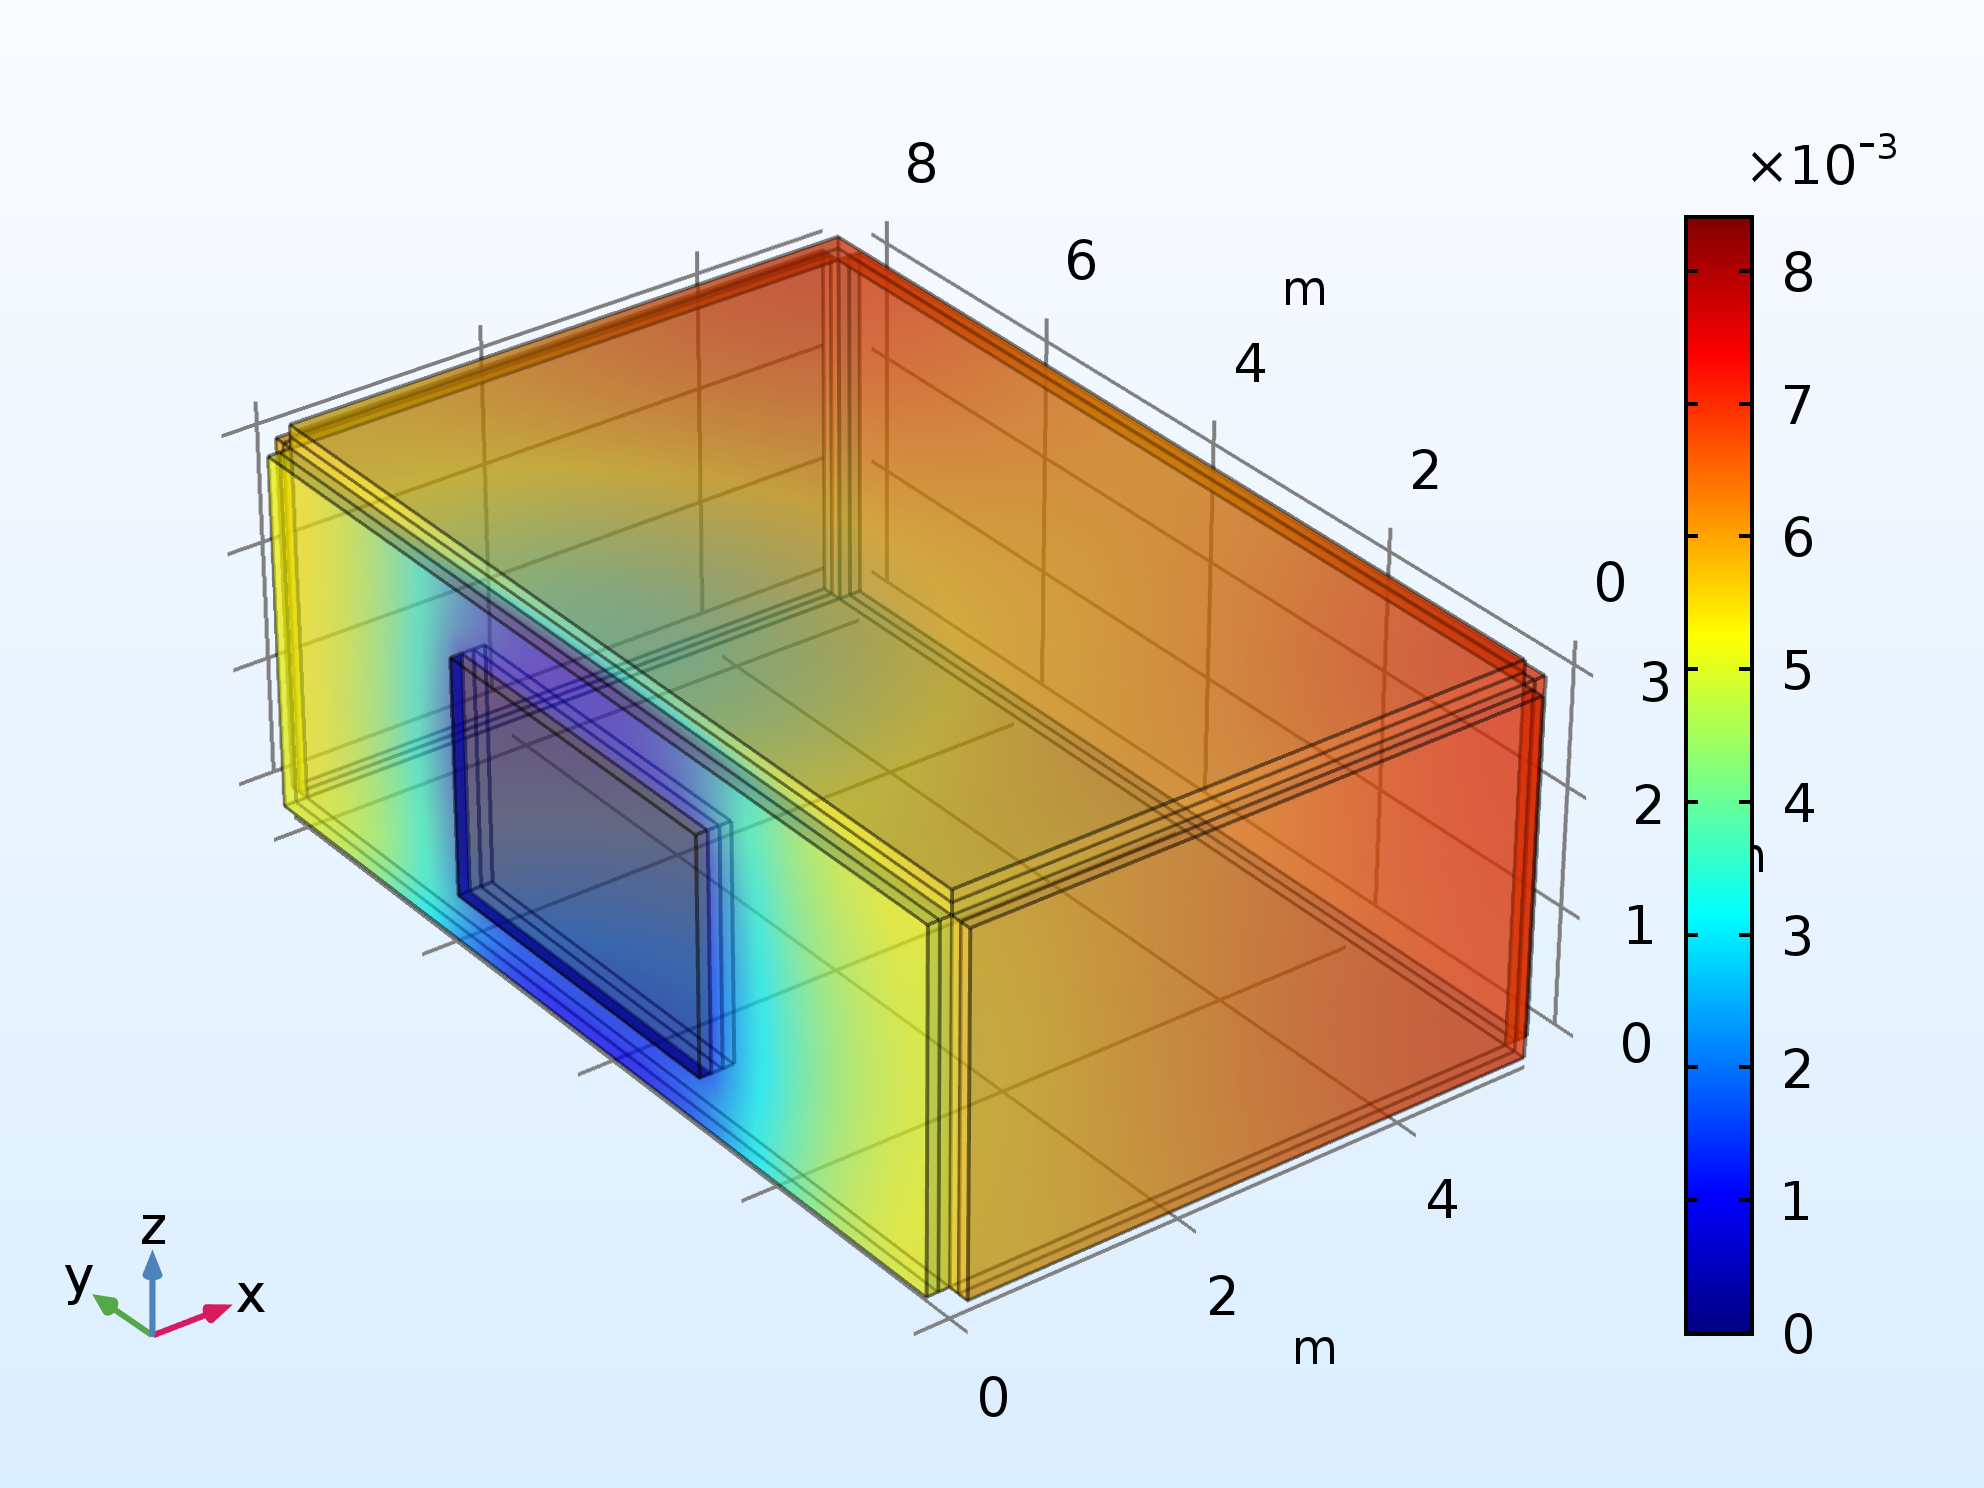
\includegraphics[width=\linewidth]{3d.png}
    \caption{$d$=3}
  \end{subfigure}
  \begin{subfigure}[b]{0.3\linewidth}
    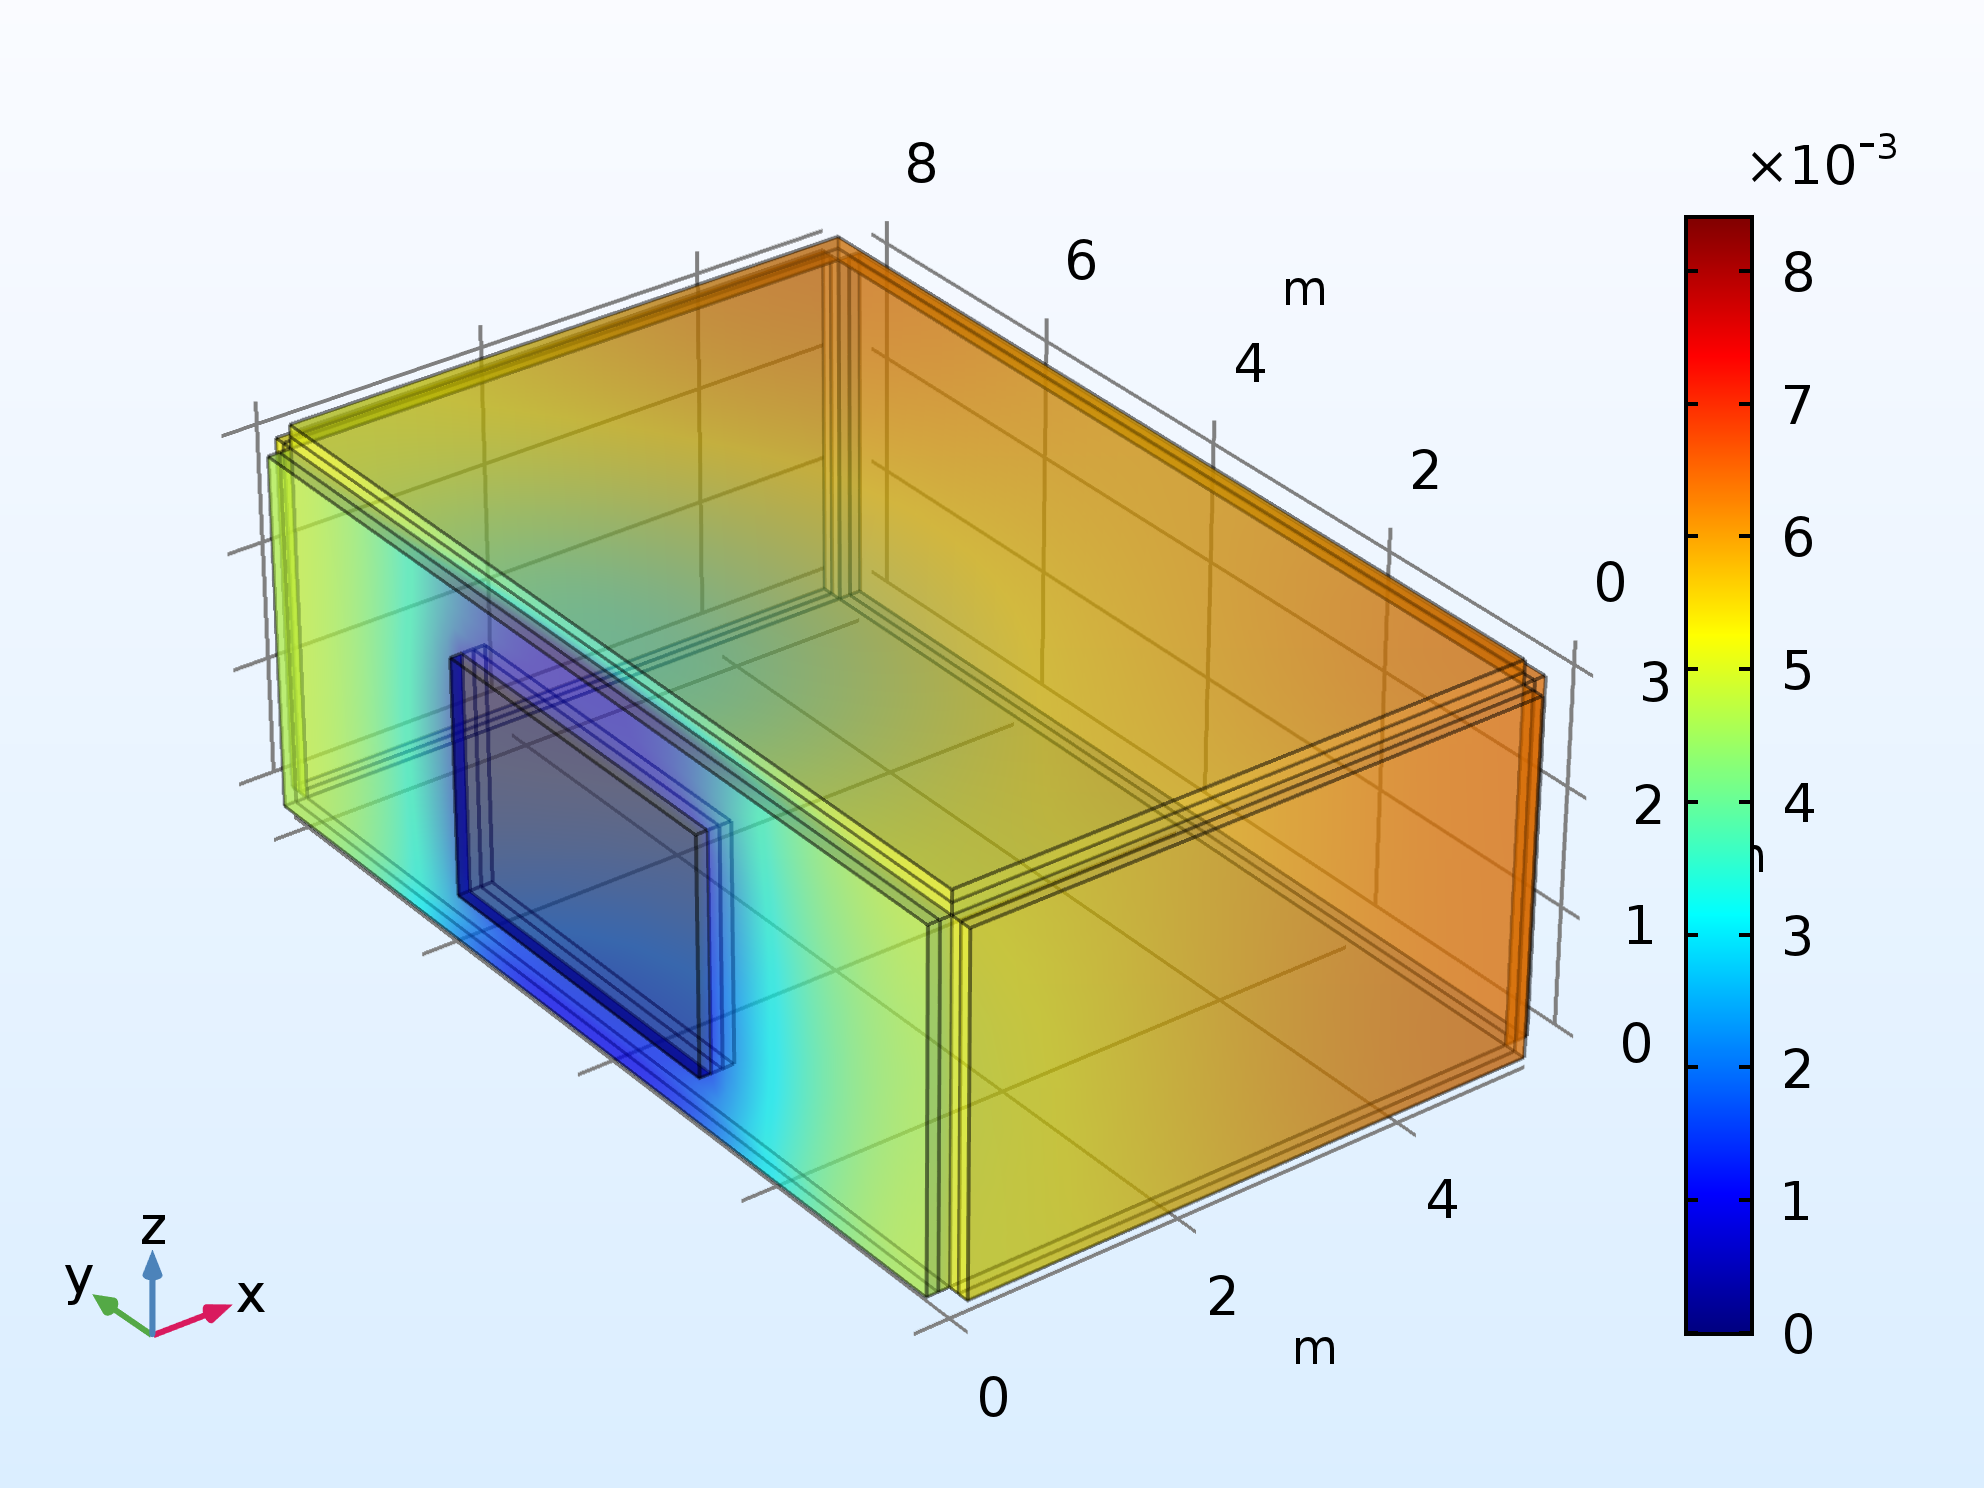
\includegraphics[width=\linewidth]{4d.png}
    \caption{$d$=4}
  \end{subfigure}
  \begin{subfigure}[b]{0.3\linewidth}
    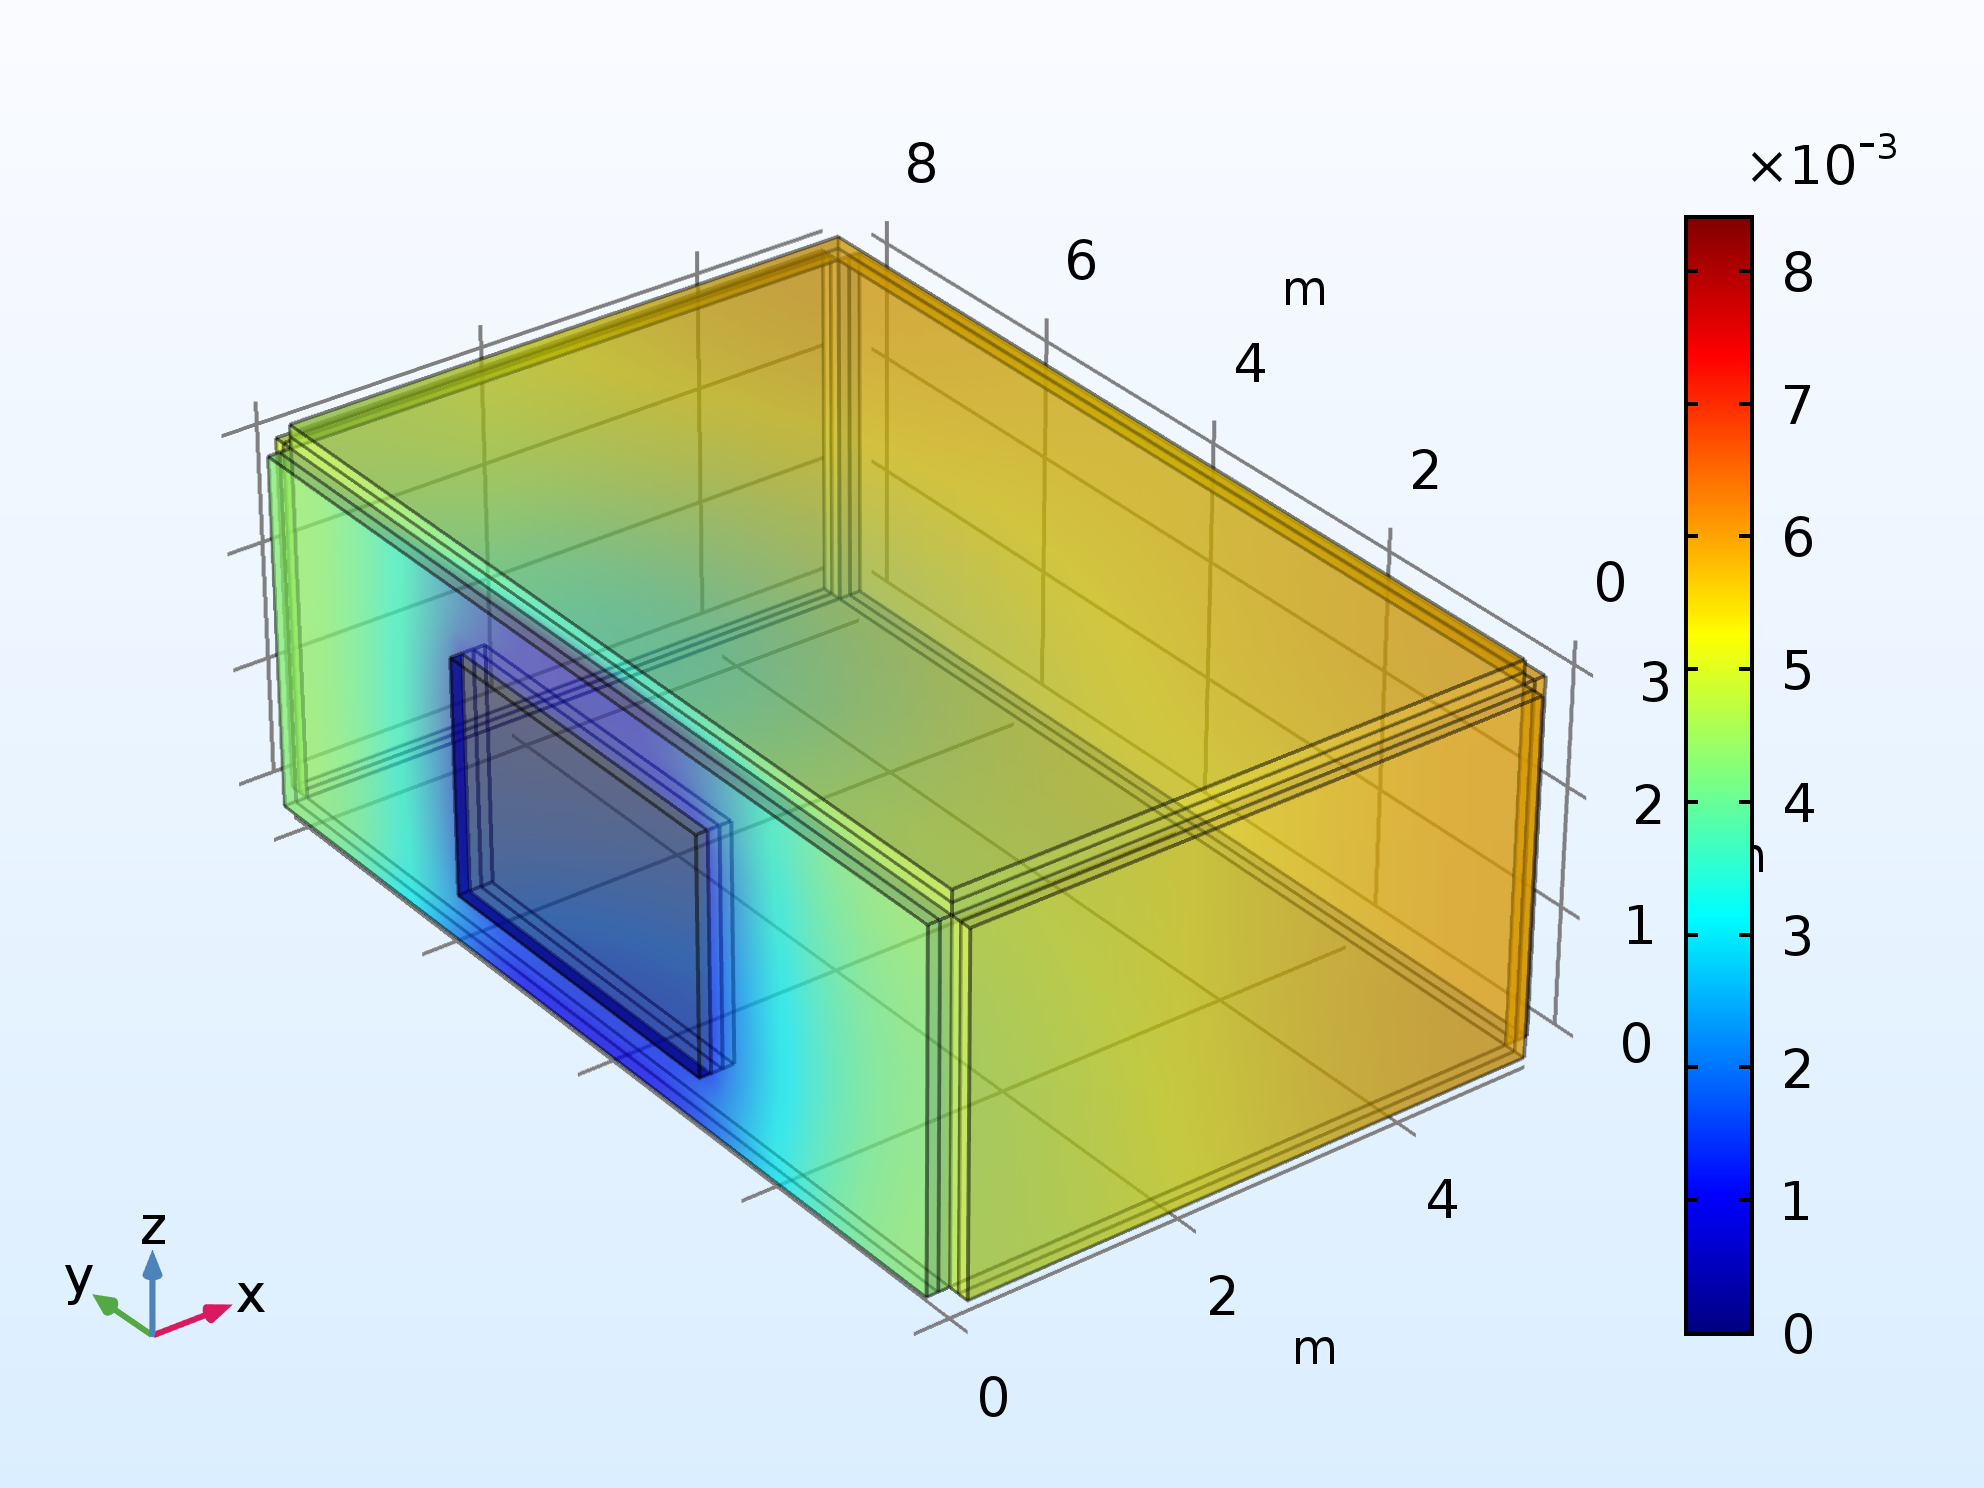
\includegraphics[width=\linewidth]{5d.png}
    \caption{$d$=5}
  \end{subfigure}
  \caption{Simulation of the window opening}
  \label{fig:window}
\end{figure}

 As can be shown above, windows make a difference to the reducing of the formaldehyde, especially in the first week after decoration. It still works well when the density of the formaldehyde is lower than the health threshold, the change of average density of formaldehyde can be shown in Figure \ref{fig:ow} , notice that the second diagram's vertical axis are set to be logarithm.
 
 \begin{figure}[H]
  \centering
  \begin{subfigure}[b]{\linewidth}
    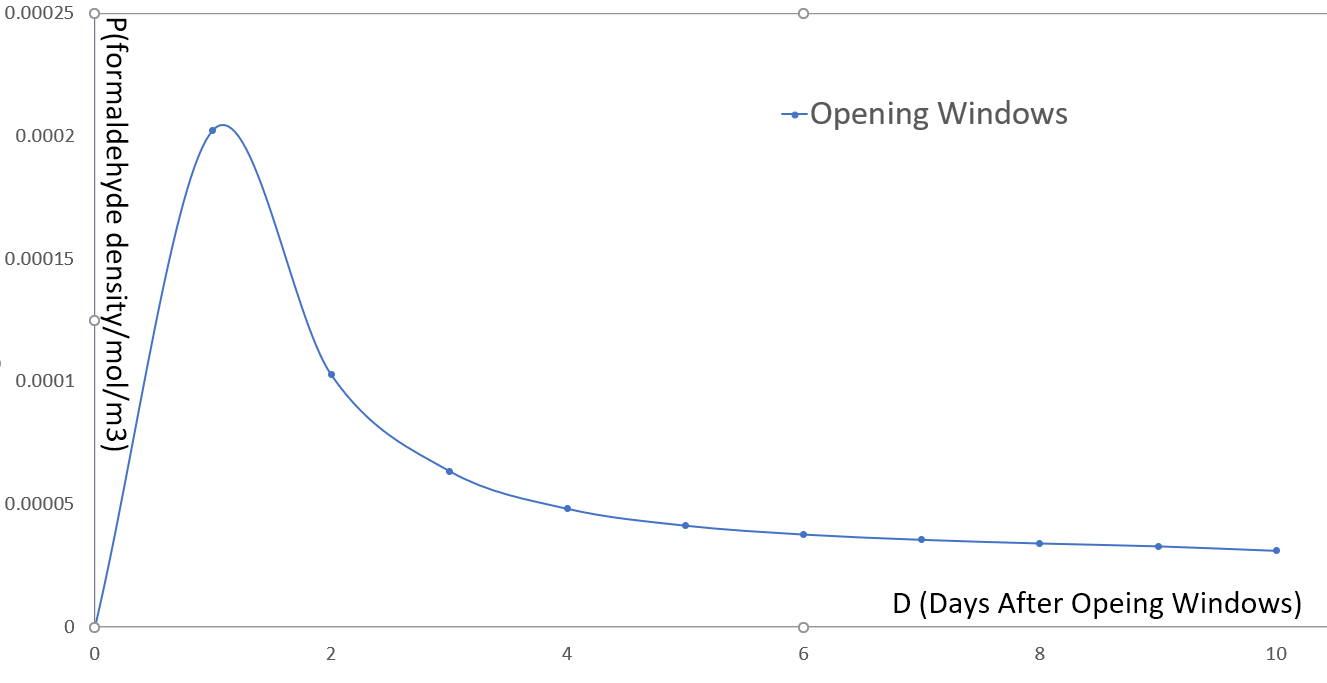
\includegraphics[width=\linewidth]{ow30-.png}
    \caption{the change in first 10 days}
  \end{subfigure}\\
  \begin{subfigure}[b]{\linewidth}
    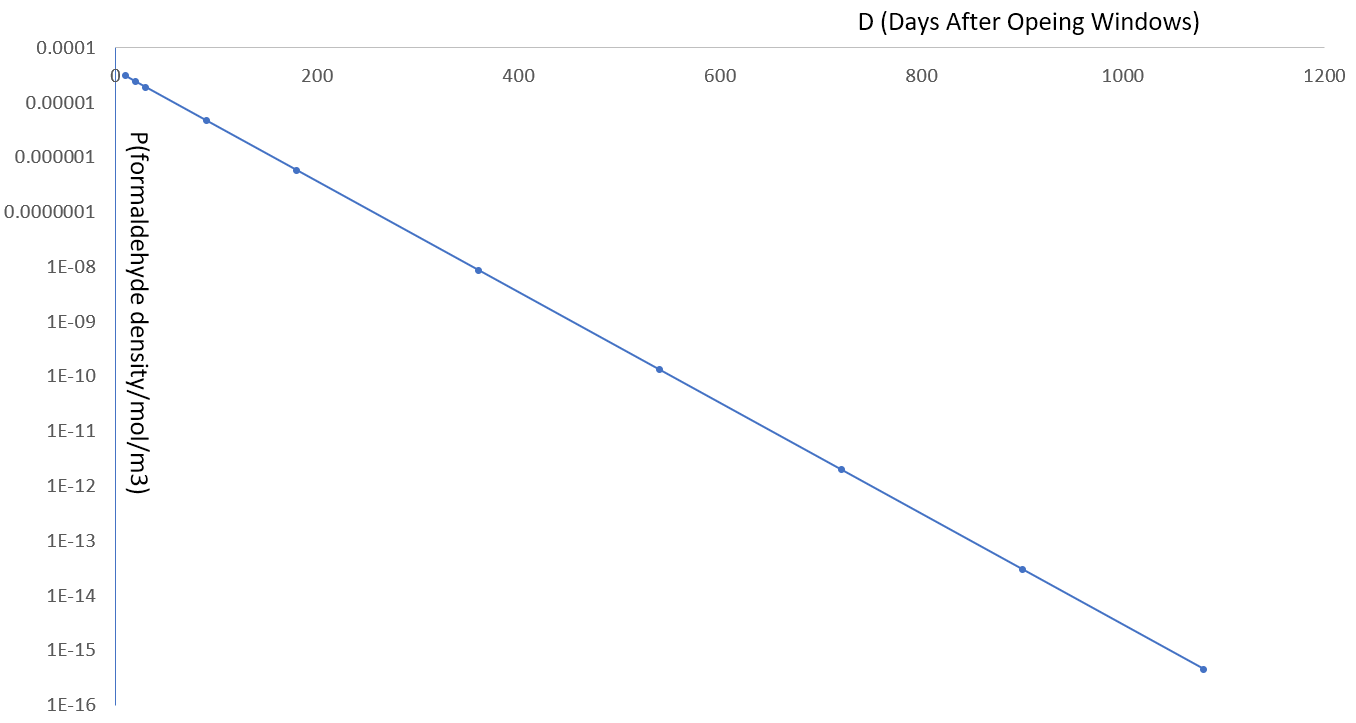
\includegraphics[width=\linewidth]{ow30+.png}
    \caption{the change after first 10 days}
  \end{subfigure}
  \caption{The change of density in 3 years (Opening Windows)}
  \label{fig:ow}
\end{figure}

As the result shows, the density of formaldehyde first increase as the walls starting to release the gas. It reaches the top after 1.5 day, from when it starts to fall down and the its derivative's absolute value also falls down. It follows a negative logarithm law and the density reach the health threshold in 106 days. From the data, we can know that opening windows makes a difference but its contribution is limited as it takes a long time to reach the health threshold. However, this strategy is the most energy-saving one. Being combined with other more effective strategies will work better.

 
\subsection{Exhausting Fans}

Opening exhausting fans is a quite effective method from our intuition because most place take it as a significant way of ventilation. We simulate an exhausting fans with a constant wind velocity and compare it to opening the windows alone, the results are shown in Figure \ref{fig:compare}. From the curve we can clearly find out that using exhausting fans is much more effective than opening windows. The maximum value is $0.00005$ when exhausting fans are turned on while this value equals $0.0002$ when opening windows. From the fitting curve we can know that it only takes 21 days for the density of formaldehyde to decline to threshold compared to the 161 days of window-opening.

\begin{figure}[H]
  \centering
  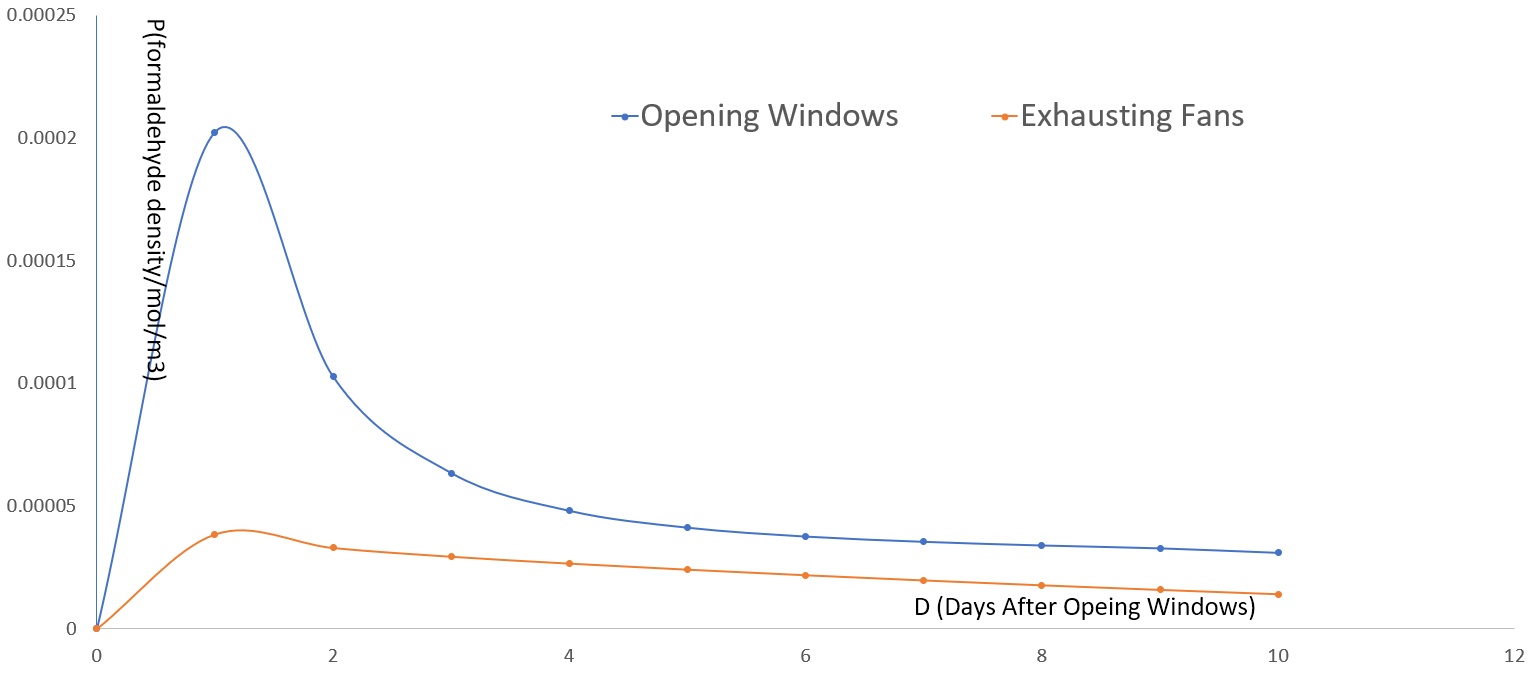
\includegraphics[width=\textwidth]{compare.png}
  \caption{Exhausting Fans Compare to Opening Windows}
  \label{fig:compare}
\end{figure}

\subsection{Temperature and Humidity}
According to our test results, the rise of temperature and increase of humidity have a synergistic effect on the increase of concentration of formaldehyde in the room. 

We simulated the diffusion of the formaldehyde under  different temperature ranging from 10$^{\circ}$C  to 35$^{\circ}$C. It turns out that under 19$^{\circ}$C the emission of formaldehyde can be controlled at an relatively low level.However, when the temperature is higher than 19$^{\circ}$C , every increase of 5$^{\circ}$C in temperature results in the rise of 1.3 to 2.5 times the concentration of formaldehyde.\cite{zhang2006temp}

On the other hand, when we increase the relative humidity by every 20 percent, the density of formaldehyde increase by 1.1 to 1.3 times.

\subsection{Other Strategies}
Besides the strategies we put forward above, there are quite a few other ways to cut down the production of formaldehyde and accelerate the emission, Here are other selected ways to make a difference:

\begin{itemize}
    \item Shop smart for furniture and cabinets, find Wood products that meet regulations
    \item Choose paints wisely and skip the wallpapers, stop using carpet from re-emitting
    \item Fill your room with formaldehyde-absorbing plants\cite{wolverton1993plants}
\end{itemize}

\subsection{Final Evaluation}
 Among all the strategies we mentioned above, it's no denying that the exhausting fans works the best although it costs energy the most. Opening windows is the most energy-friendly way and it works well the same. Keeping temperature and humidity also works but the energy costs will be high. Other strategies can be adopted in some specific situation.
 
 To strike a balance between effectiveness and energy cost, we strongly recommend householders to open exhausting fans in the first few days and open the window simultaneously. After the first few days, householders can stop using the exhausting fans and turn to opening windows while adopt some other strategies such as fill the room with formaldehyde-absorbing plants.

\section{Model Analysis}
\subsection{Sensitivity Analysis}
Note that our model consists a lot parameters such as room temperature and the volume of the room. Now we are studying the impact of these two parameters on the declining curve of concentration of formaldehyde and $t_{threshold}$, using CF model with a window.

\subsubsection{Impact of Volume}

In this section we ignore the impact of shape and concentrate on a series of similar cuboid room with linear scaling.
\begin{table}[H]
  \begin{center}
    \caption{Selected volume.}
    \label{tab:Not}
    \begin{tabular}{ccc}
      	\toprule
      	Scale & Size(m) & Volume(m$^3$)\\
      	\midrule
        0.8&$6.4\times4.0\times2.4$& $61.44$\\
        0.9&$7.2\times4.5\times2.7$& $87.48$\\
    	1.0&$8.0\times5.0\times3.0$& $120.00$\\
        1.1&$8.0\times5.0\times3.0$& $159.72$\\
        1.2&$8.0\times5.0\times3.0$& $207.36$\\
      	\bottomrule
    \end{tabular}
  \end{center}
\end{table}

\begin{figure}[H]
  \centering
  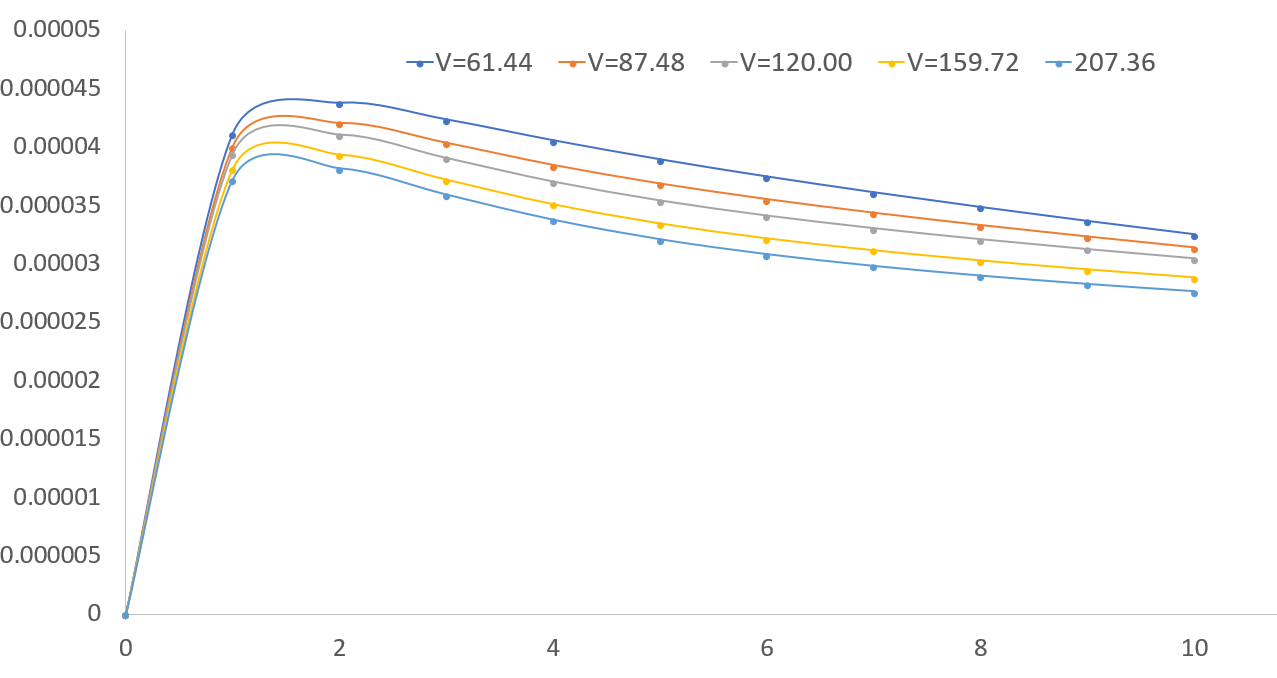
\includegraphics[width=\textwidth]{volume.png}
  \caption{Impact of Volume}
  \label{fig:volume}
\end{figure}

As the curve of volume shows, the density's change pattern varies when the volume differs. When the volume is high, the maximum value is lower. However, compared to the volume change itself, the change of density is minor. In the meantime, the relation between volume and $t_{threshold}$ is shown in Table \ref{tab:RbV}, in which we can see that larger house needs much longer time to be healthy for people to live in.

\begin{table}[H]
  \begin{center}
    \caption{Relation between volume and $t_{threshold}$.}
    \label{tab:RbV}
    \begin{tabular}{lccccc}
      	\toprule
        Volume(m$^3$) & 61.44 & 87.48 & 120.00 & 159.72 & 207.36\\
		\midrule
        $t_{threshold}$(s) & 88 & 98 & 106 & 114 & 122\\
      	\bottomrule
    \end{tabular}
  \end{center}
\end{table}



\subsubsection{Impact of Temperature}
Considered that the range that an air conditioner can adjust, we think considering step of temperature as $5^o$C is reasonable. Meanwhile, using Gilliland's semiempirical\cite{christian1959sublimation} equation:
\begin{equation}
D_{12}=435.7\frac{T^{3/2}}{p_0(V_1^{1/3}+V_2^{1/3})^2}\sqrt{\frac{1}{M_1}+\frac{1}{M_2}} \mathrm{cm}^2/s
\end{equation}
We know that the diffusion coefficient is proportional to $T^{3/2}$ in a narrow range, so we can know the diffusion coefficient of temperature varying from $283.15$K to $313.15$K.

\begin{table}[H]
  \begin{center}
    \caption{Diffusion Coefficient.}
    \label{tab:DC}
    \begin{tabular}{lccccccc}
      	\toprule
      	T(K) & 283.15 & 288.15 & 293.15 & 298.15 & 303.15 & 308.15 & 313.15\\
      	\midrule
        D($10^{-5}$cm$^2/s$) & 1.67 & 1.71 & 1.75 & 1.80 & 1.85 & 1.89 & 1.94\\
      	\bottomrule
    \end{tabular}
  \end{center}
\end{table}



From the results shown in Figure \ref{fig:temp}, we can conclude that temperature has minor impact on the diffusion of formaldehyde, but we should still be aware that the higher the temperature is, the faster formaldehyde diffuses. Then we have a relation between temperature and $t_{threshold}$ in Table \ref{tab:RbT}.

\begin{figure}[H]
  \centering
  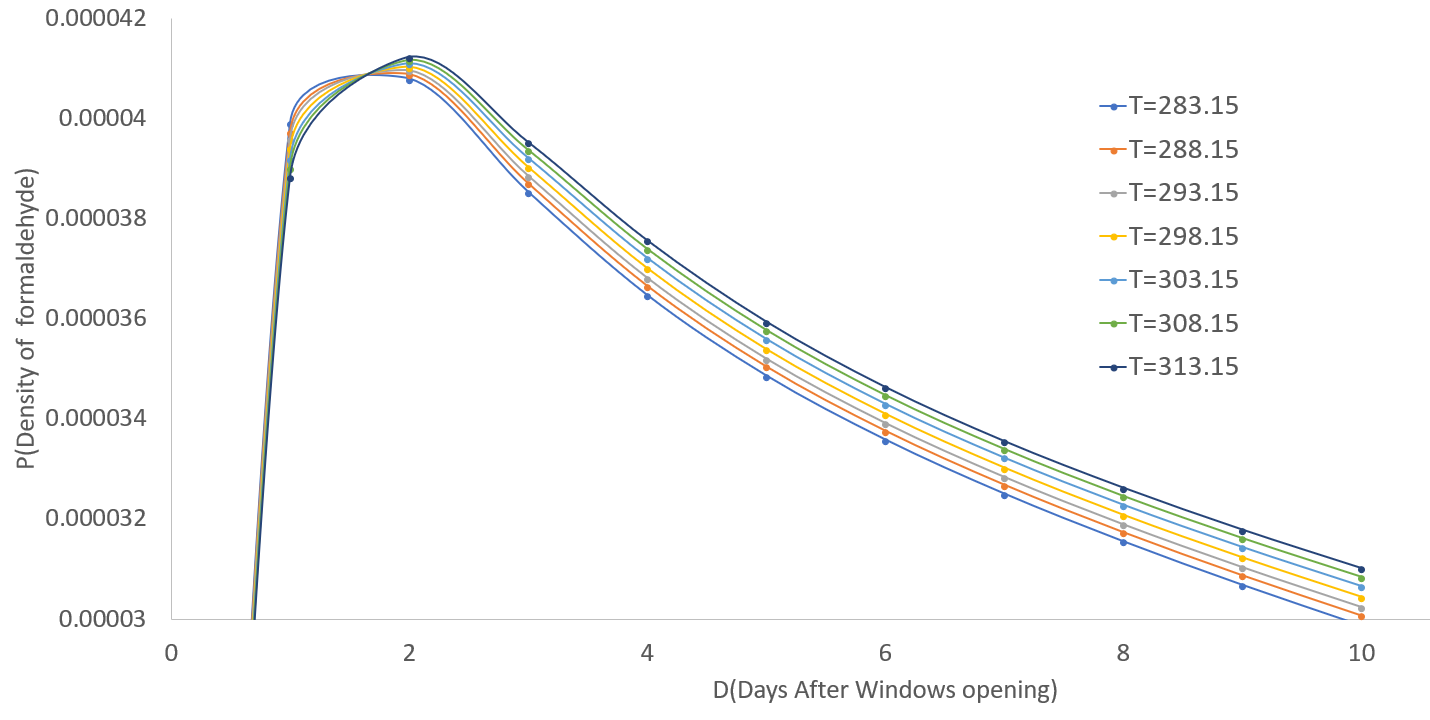
\includegraphics[width=\textwidth]{temp.png}
  \caption{Impact of Temperature}
  \label{fig:temp}
\end{figure}

As the figure of temperature shows, the concentration's curve also varies when the temperature differs. When the temperature is high, the maximum value appears quicker and starting to fall down faster. In the meantime, the relation between temperature and $t_{threshold}$ is shown in Table \ref{tab:RbT}, in which we can see that the time needed to reduce to the health threshold are shorter when the temperature are higher.

\begin{table}[H]
  \begin{center}
    \caption{Relation between temperature and $t_{threshold}$.}
    \label{tab:RbT}
    \begin{tabular}{lccccccc}
      	\toprule
      	Temperature(T) & 313.15 & 308.15 & 303.15 & 298.15 & 293.15 & 288.15 & 283.15\\
      	\midrule
        $t_{threshold}$(d) & 99 & 102 & 104 & 106 & 109 & 111 & 114\\
      	\bottomrule
    \end{tabular}
  \end{center}
\end{table}


\subsubsection{Impact of Additional Emission Sources}

Besides the wall and ceiling, additional emission sources like wooden furniture and wallpaper also influence a lot. According to a research \cite{brown1999chamber} conduct by SK Brown, some kinds of wooden material produce formaldehyde even more than latex paint and oil paint we use now. We simulate a wooden furniture in the house and simulate the distribution of the formaldehyde, the results are shown in Figure \ref{fig:sources}:

\begin{figure}[H]
  \centering
  \begin{subfigure}[b]{0.3\linewidth}
    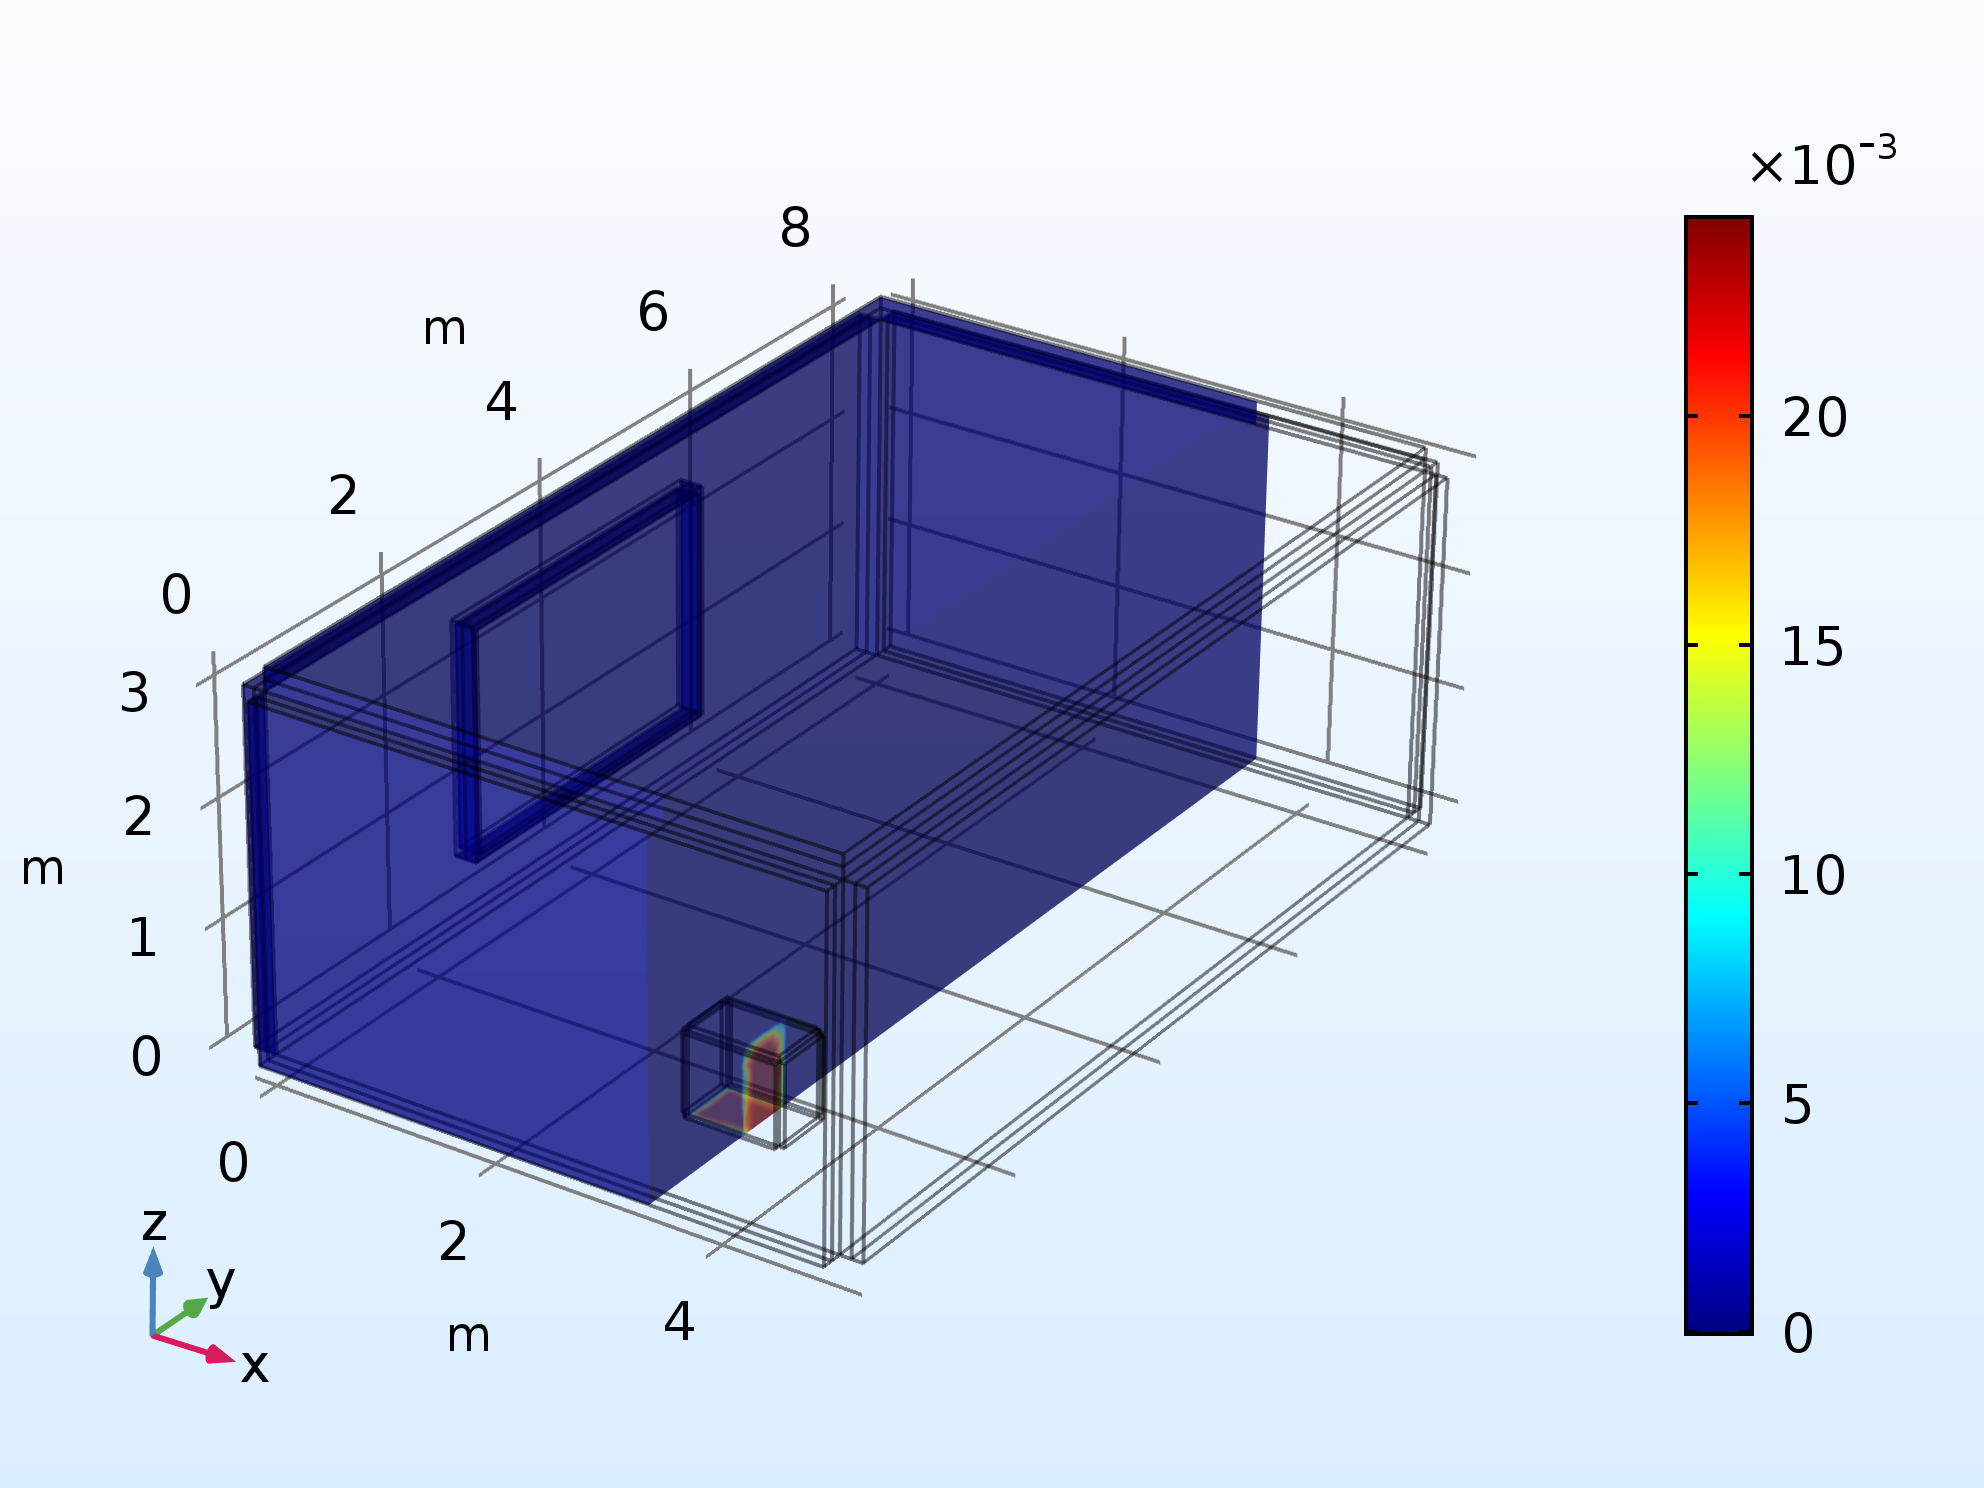
\includegraphics[width=\linewidth]{Day0.png}
    \caption{$h$=0}
  \end{subfigure}
  \begin{subfigure}[b]{0.3\linewidth}
    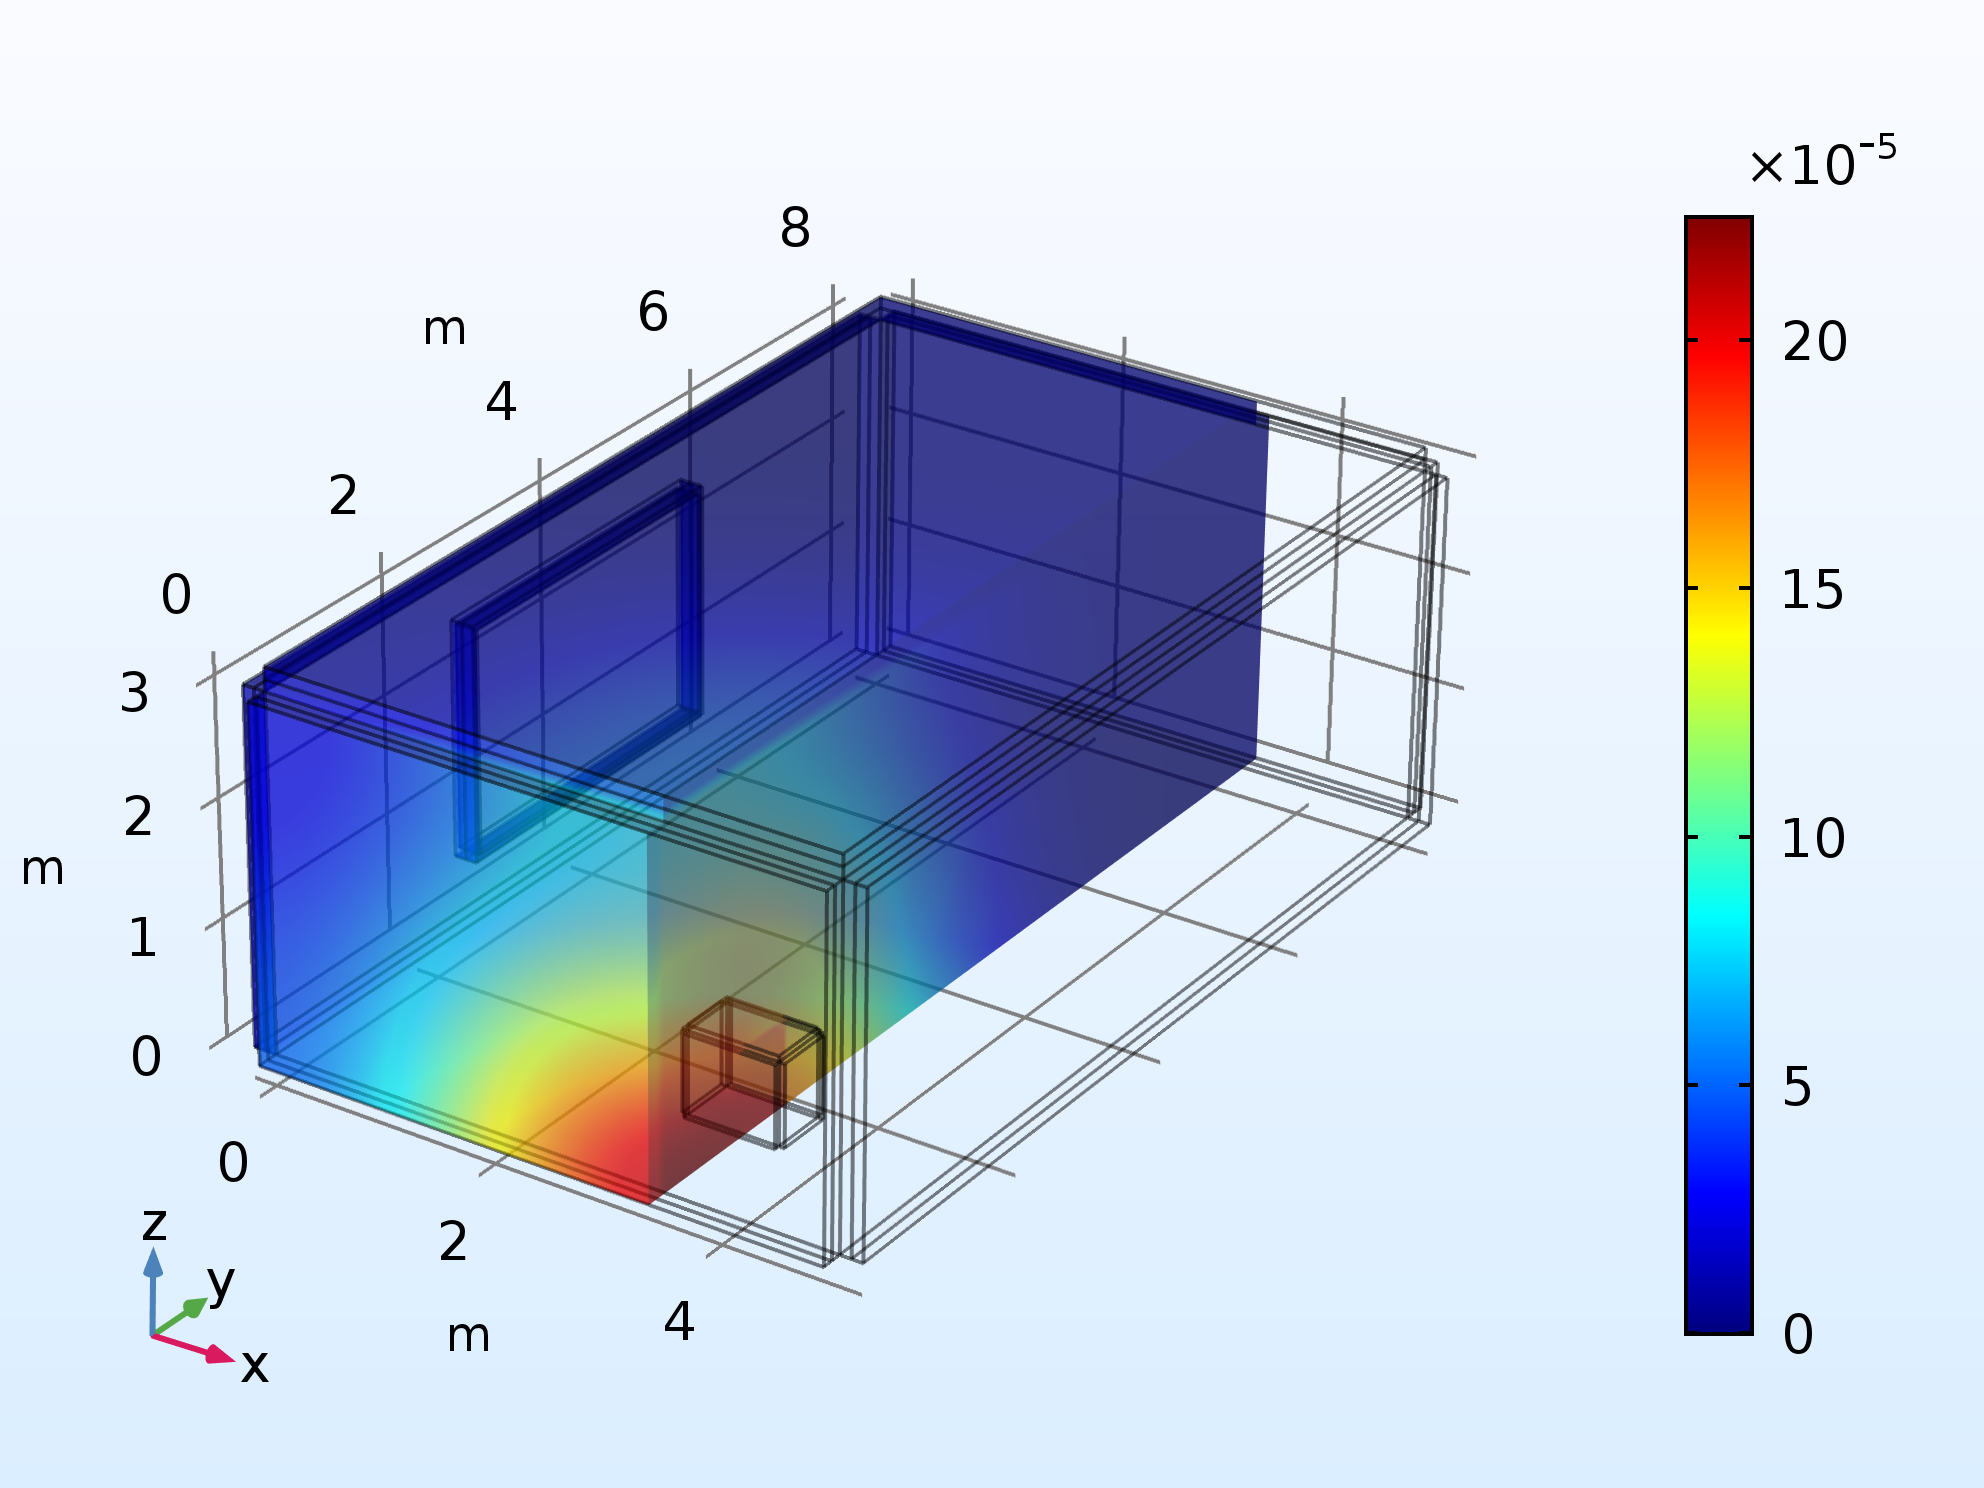
\includegraphics[width=\linewidth]{Day1.png}
    \caption{$h$=1}
  \end{subfigure}
  \begin{subfigure}[b]{0.3\linewidth}
    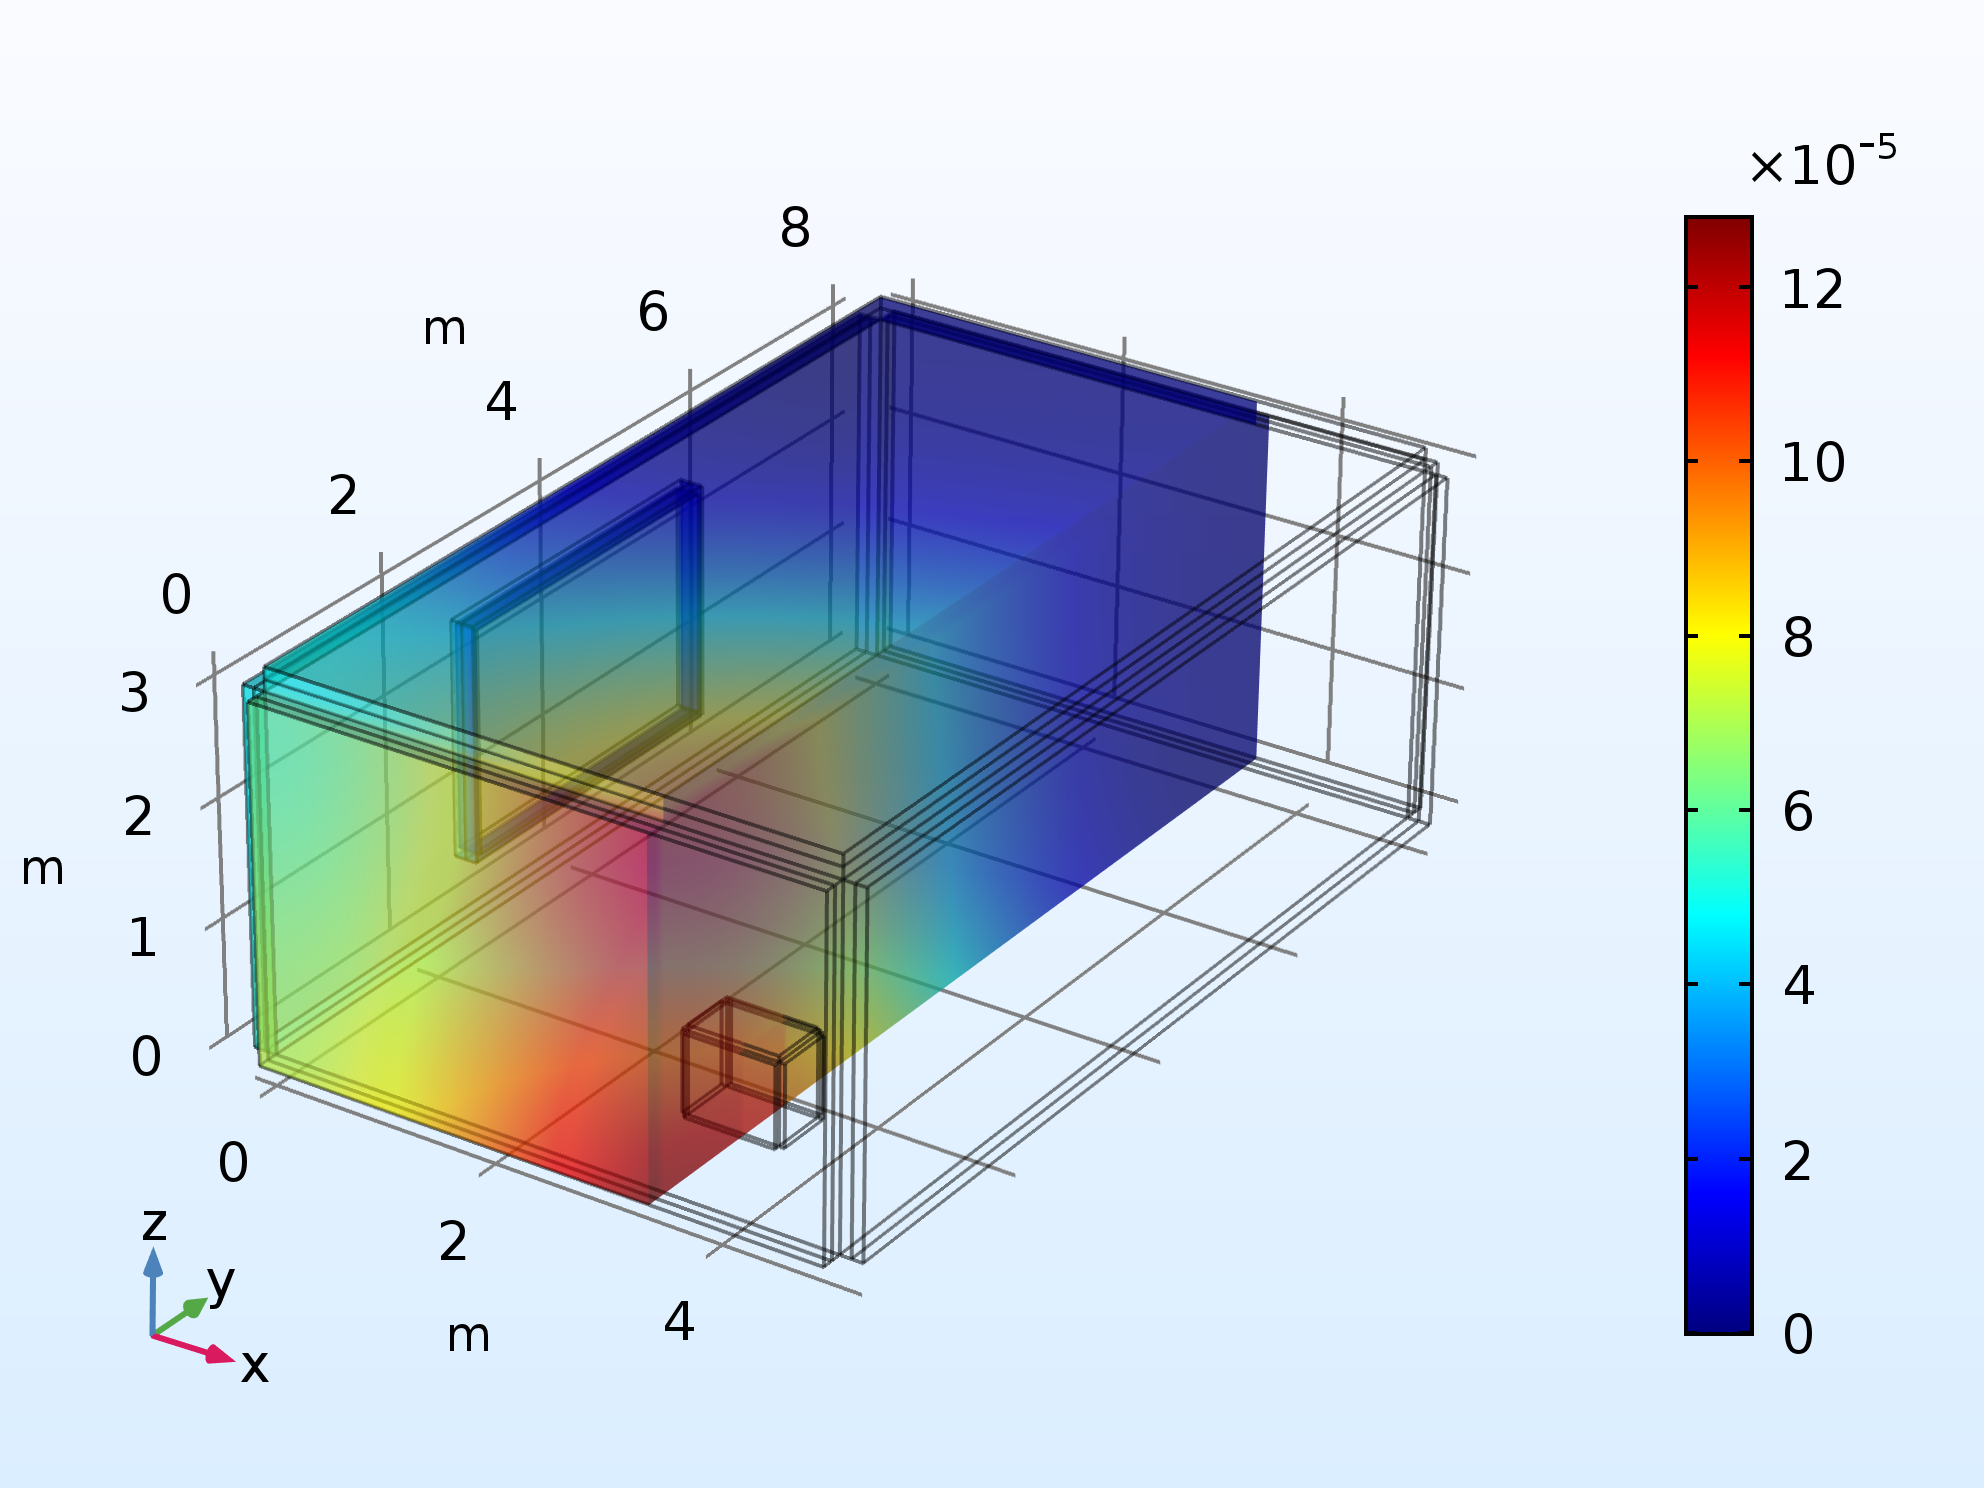
\includegraphics[width=\linewidth]{Day2.png}
    \caption{$h$=2}
  \end{subfigure}\\
  \begin{subfigure}[b]{0.3\linewidth}
    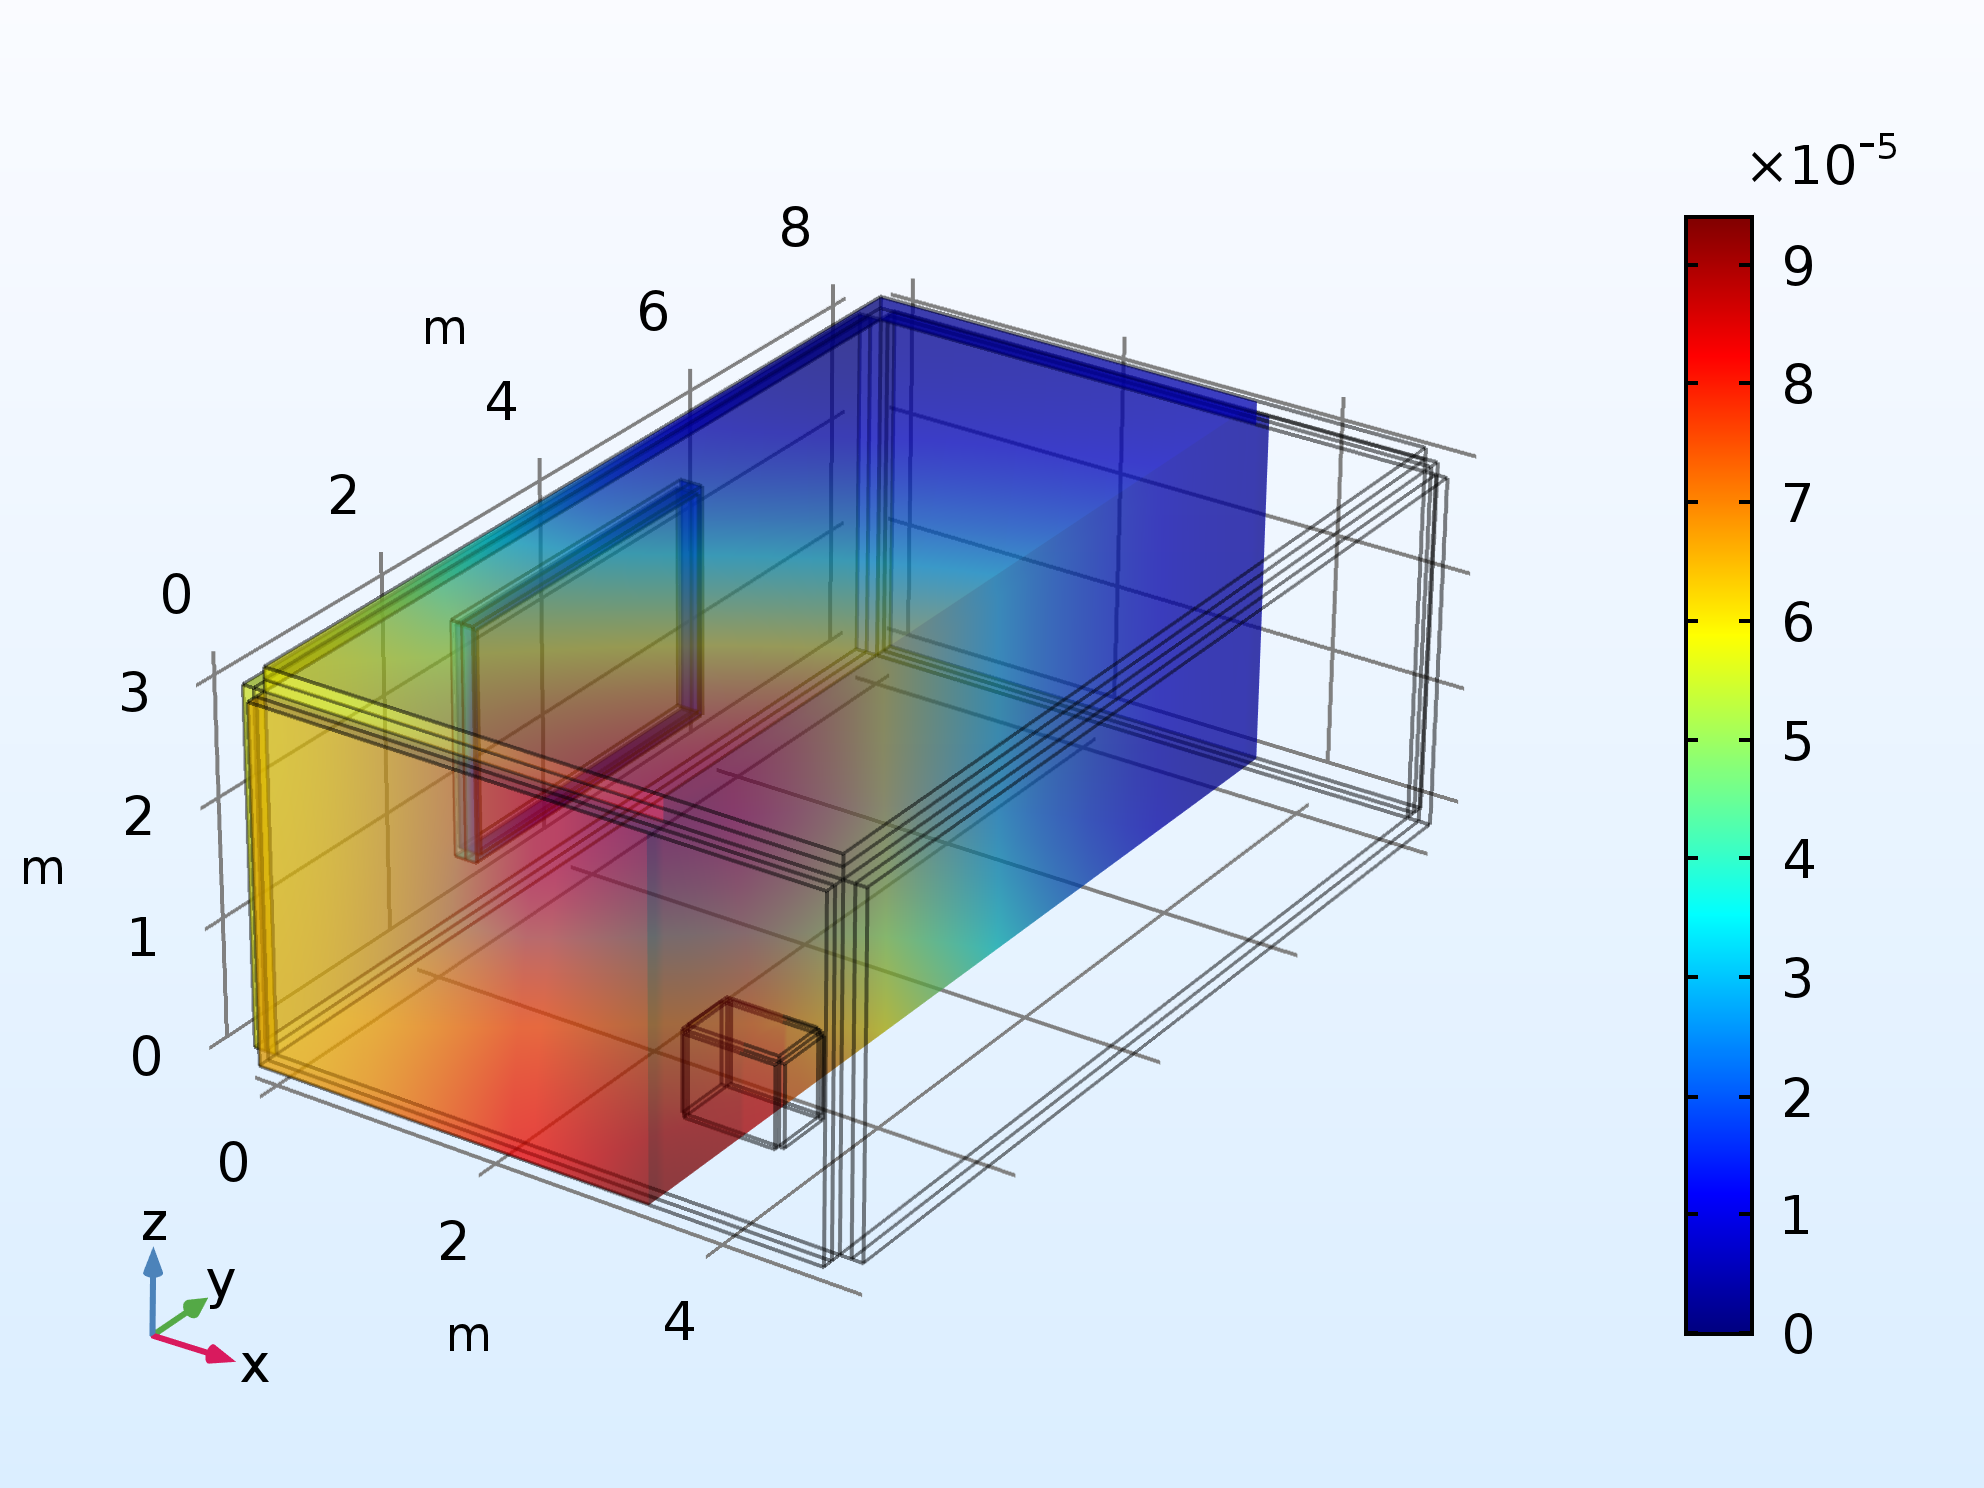
\includegraphics[width=\linewidth]{Day3.png}
    \caption{$h$=3}
  \end{subfigure}
  \begin{subfigure}[b]{0.3\linewidth}
    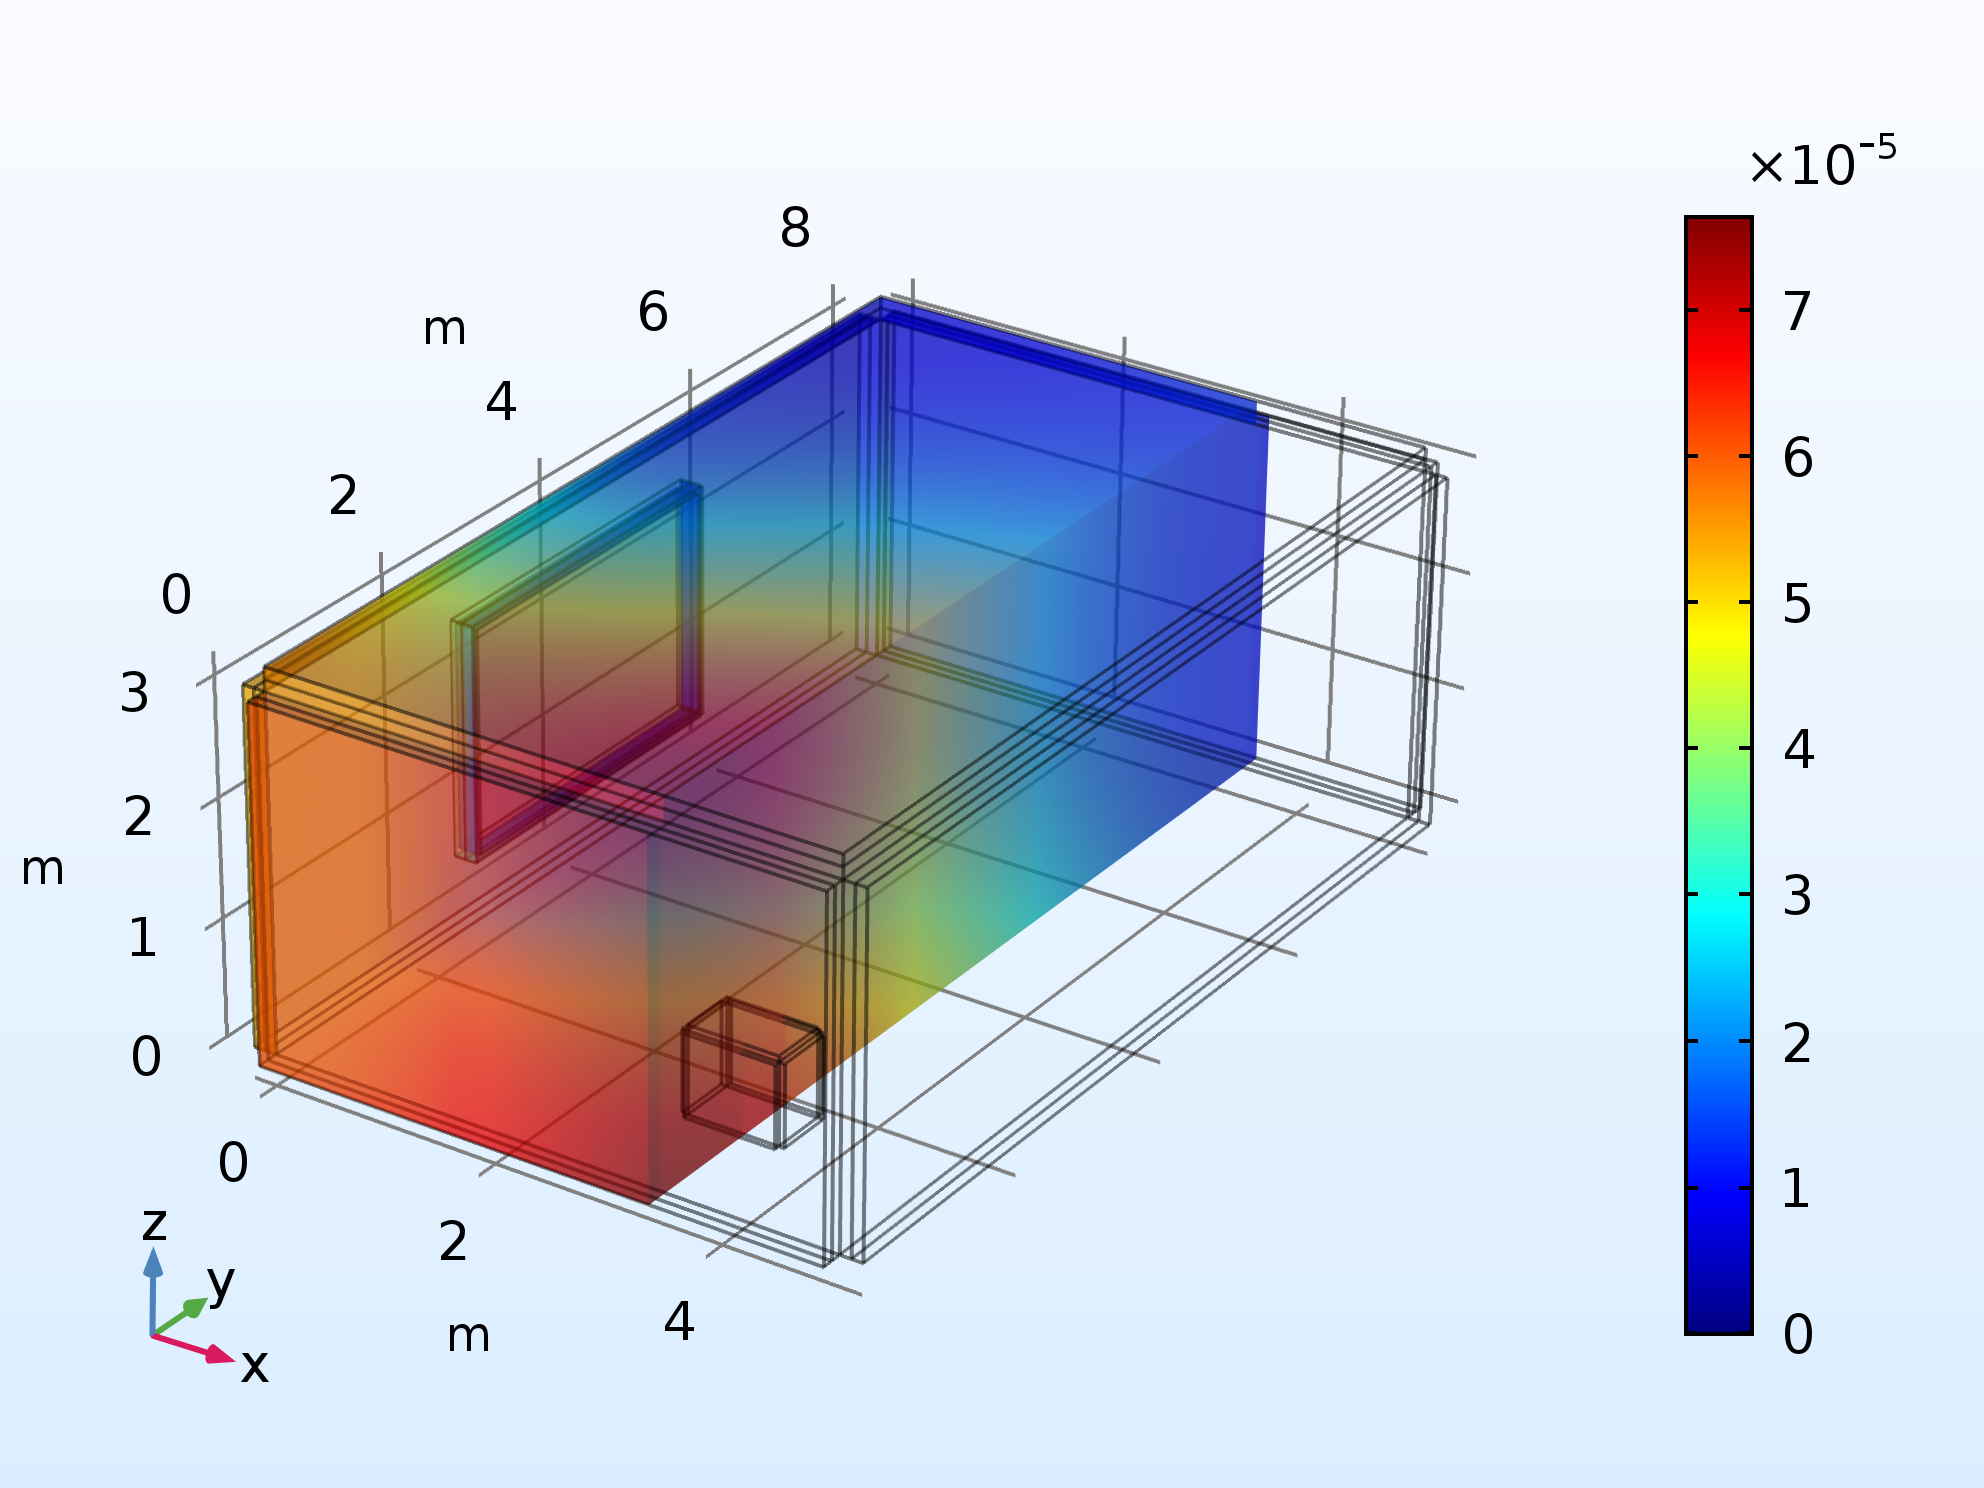
\includegraphics[width=\linewidth]{Day4.png}
    \caption{$h$=4}
  \end{subfigure}
  \begin{subfigure}[b]{0.3\linewidth}
    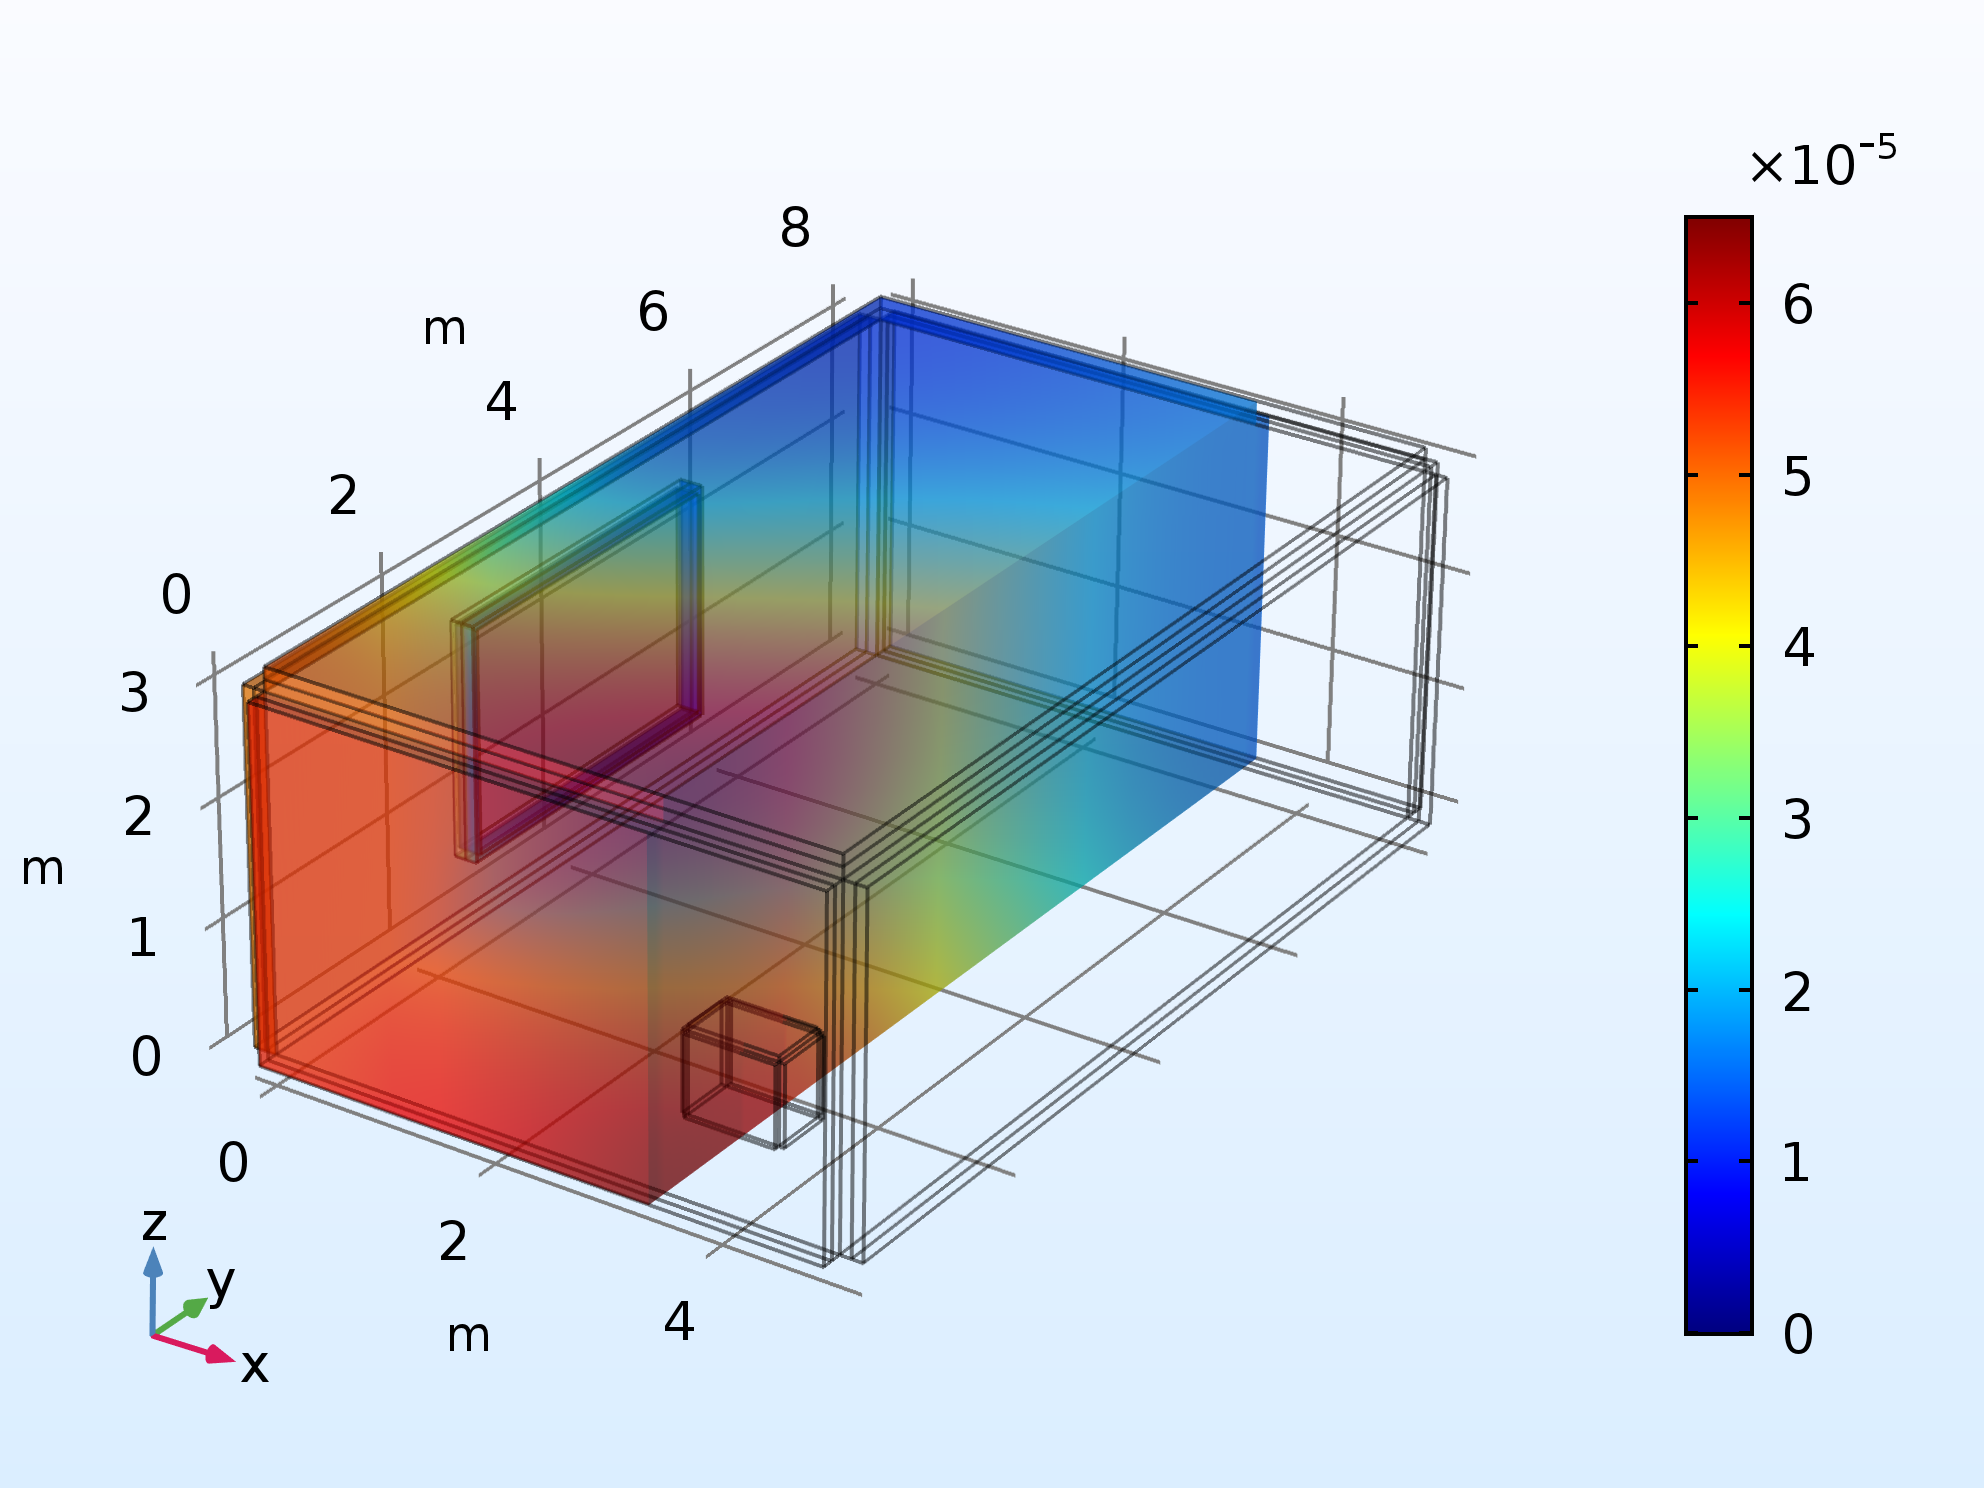
\includegraphics[width=\linewidth]{Day5.png}
    \caption{$h$=5}
  \end{subfigure}
  \caption{Simulation of the emission sources}
  \label{fig:sources}
\end{figure}


As shown in the figure above, additional emission sources will bring nonuniform distribution of formaldehyde in the house. Those space closed to the sources will have higher density of formaldehyde. Also, the degree of the influence are determined by the concentration of formaldehyde in the sources.



\subsubsection{Impact of Inner Structure}

Most houses are not simply combination of cuboid as inner structure like screens and interior walls may influence the distribution of formaldehyde. We simulate the whole process with a wall and an interior door in the house, the simulation result are shown in Figure \ref{fig:wall}:

\begin{figure}[H]
  \centering
  \begin{subfigure}[b]{0.3\linewidth}
    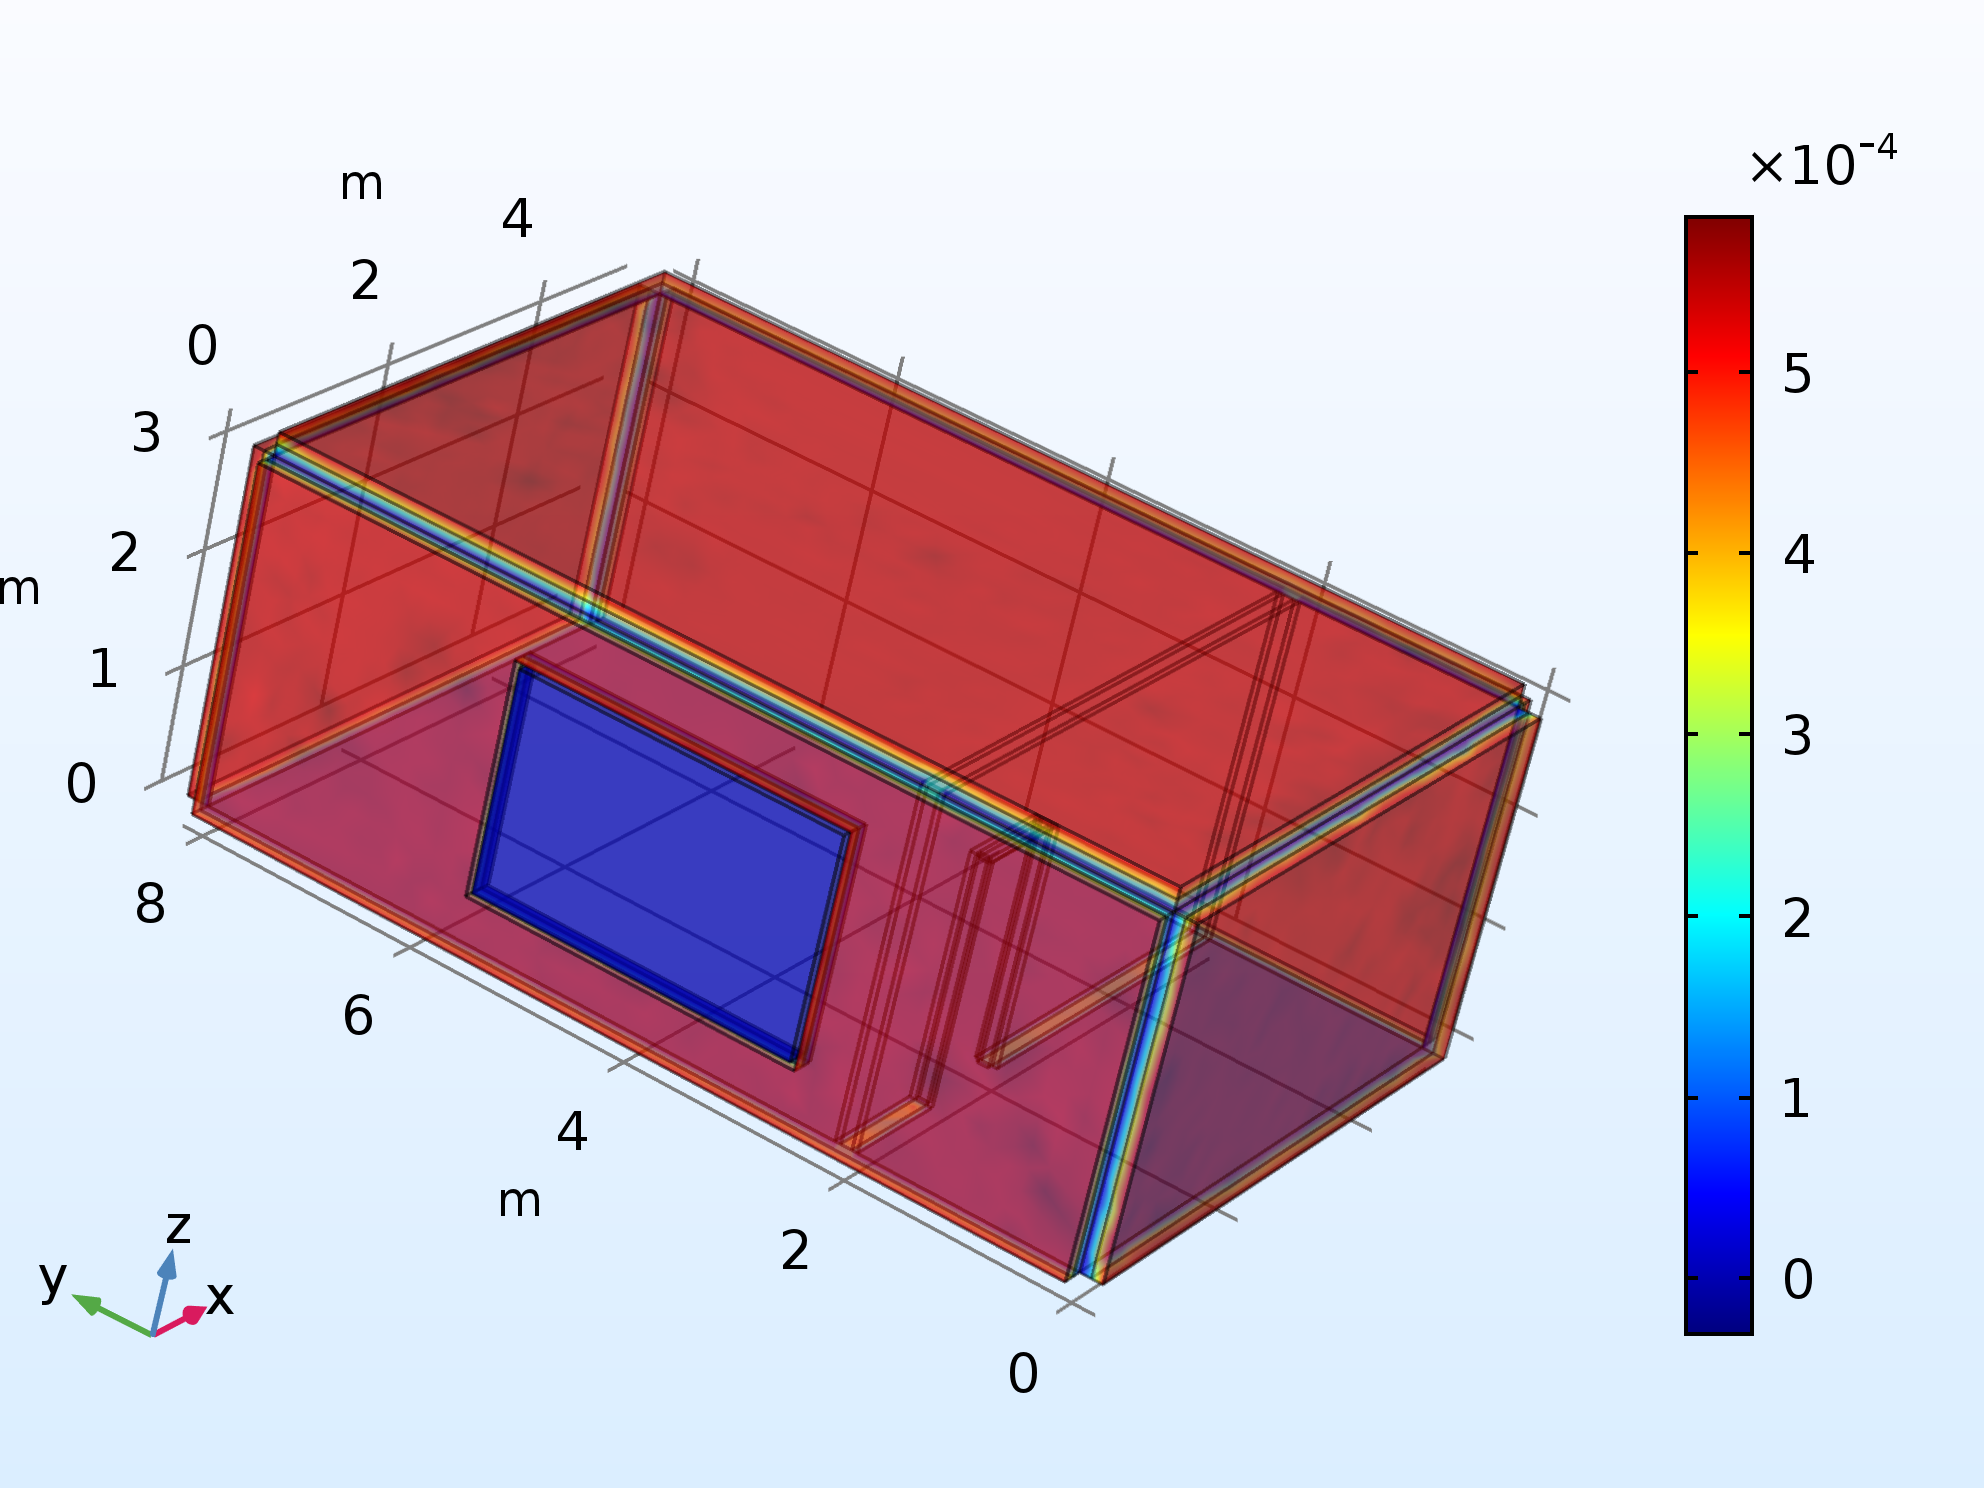
\includegraphics[width=\linewidth]{Month0.png}
    \caption{$M$=0}
  \end{subfigure}
  \begin{subfigure}[b]{0.3\linewidth}
    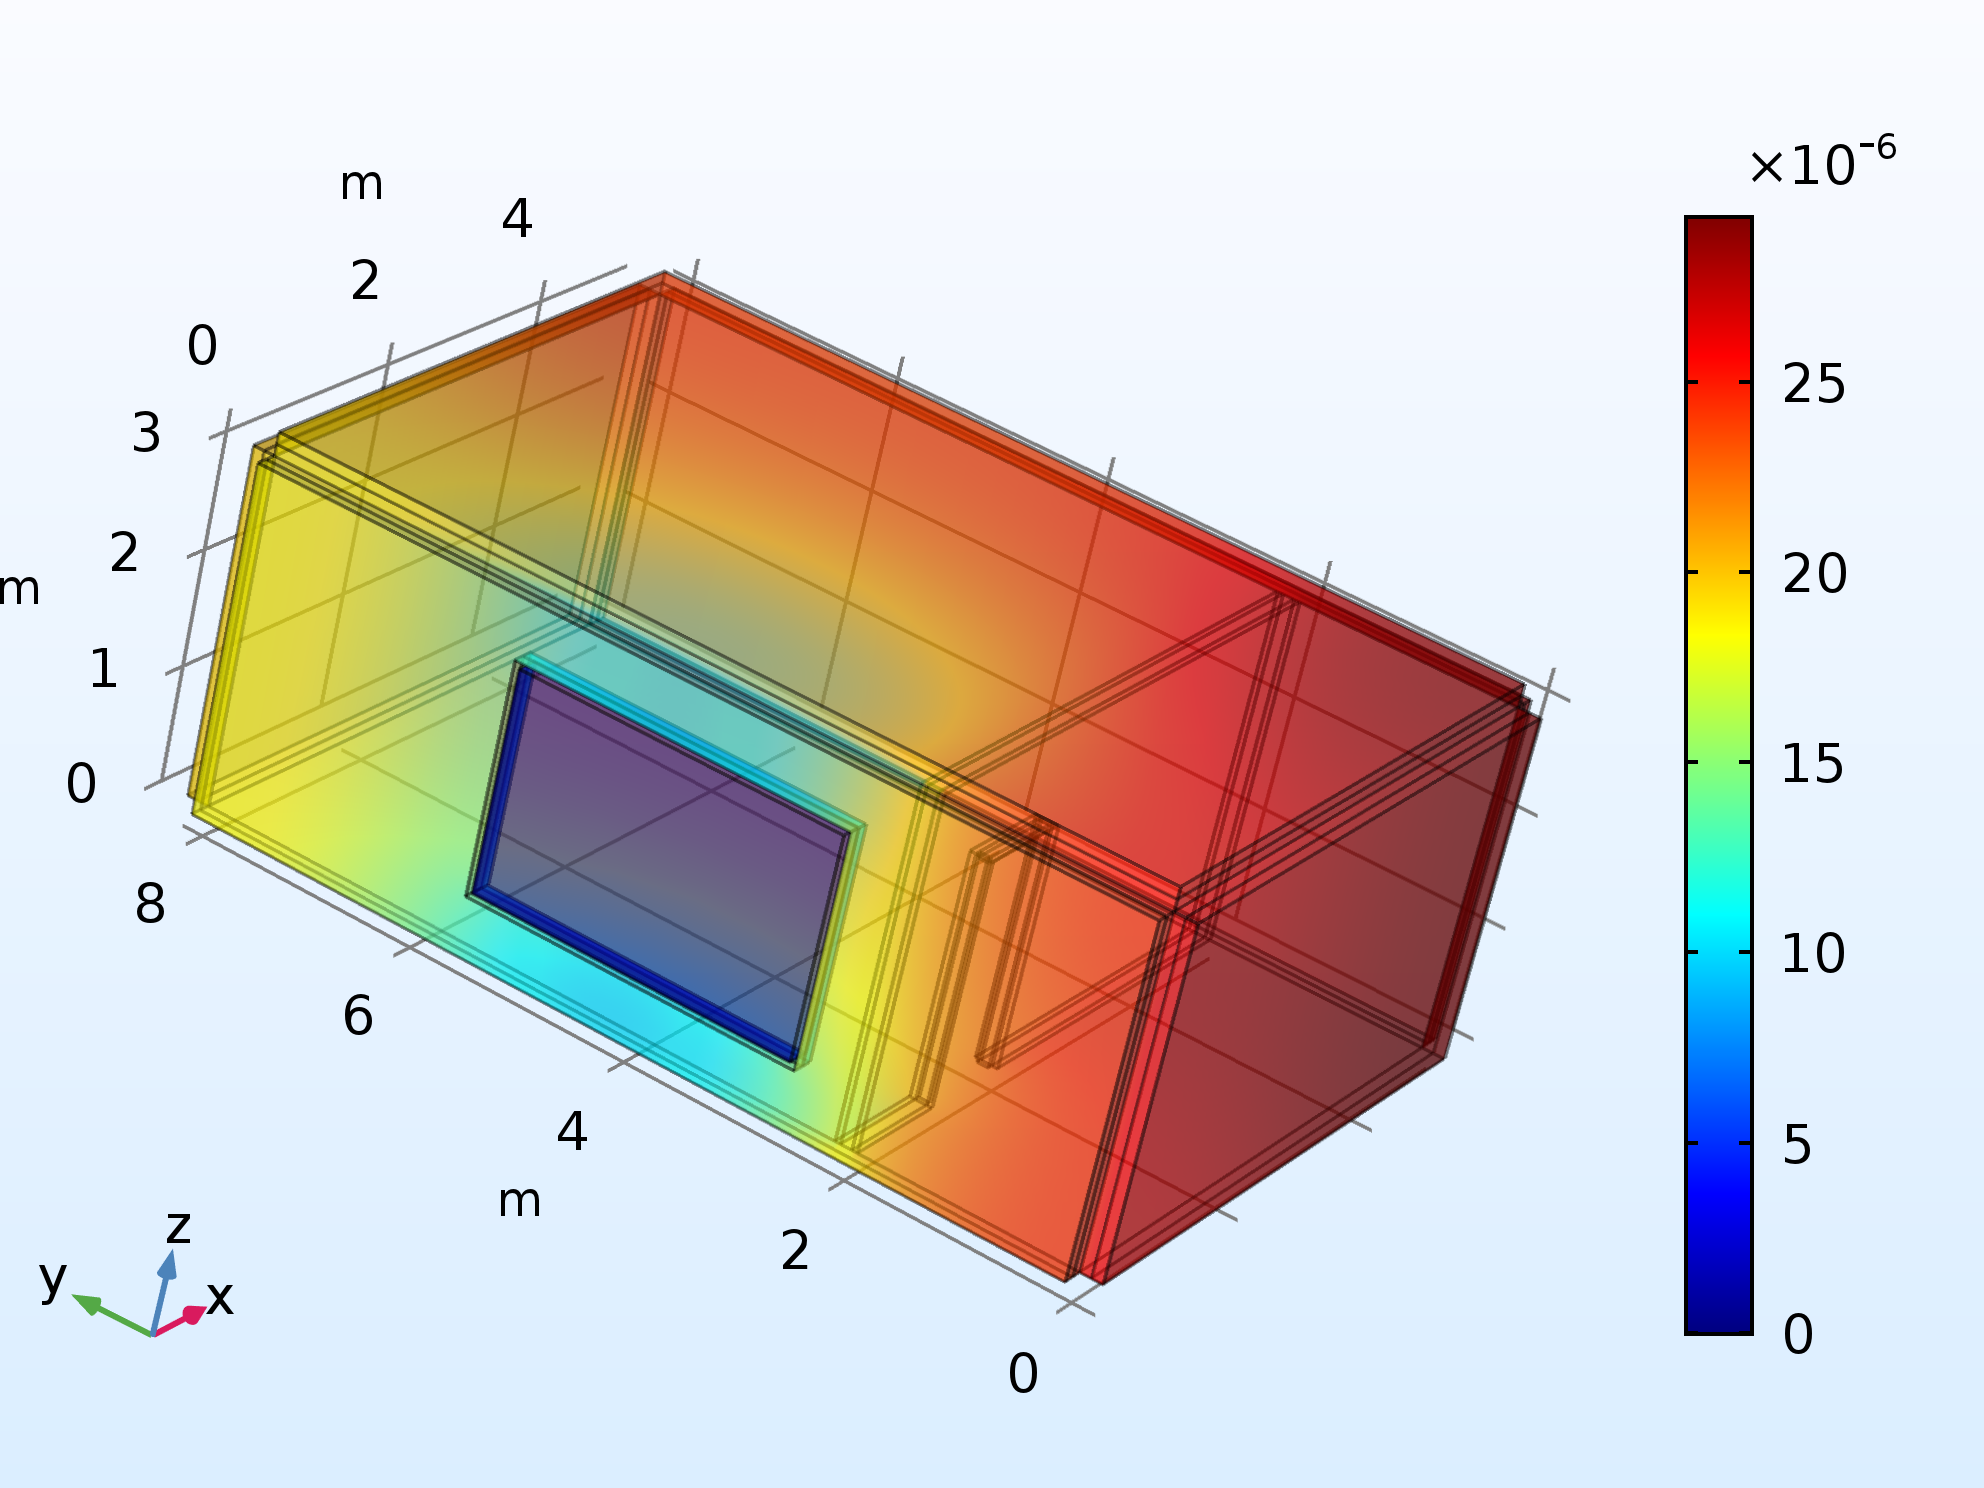
\includegraphics[width=\linewidth]{Month1.png}
    \caption{$M$=1}
  \end{subfigure}
  \begin{subfigure}[b]{0.3\linewidth}
    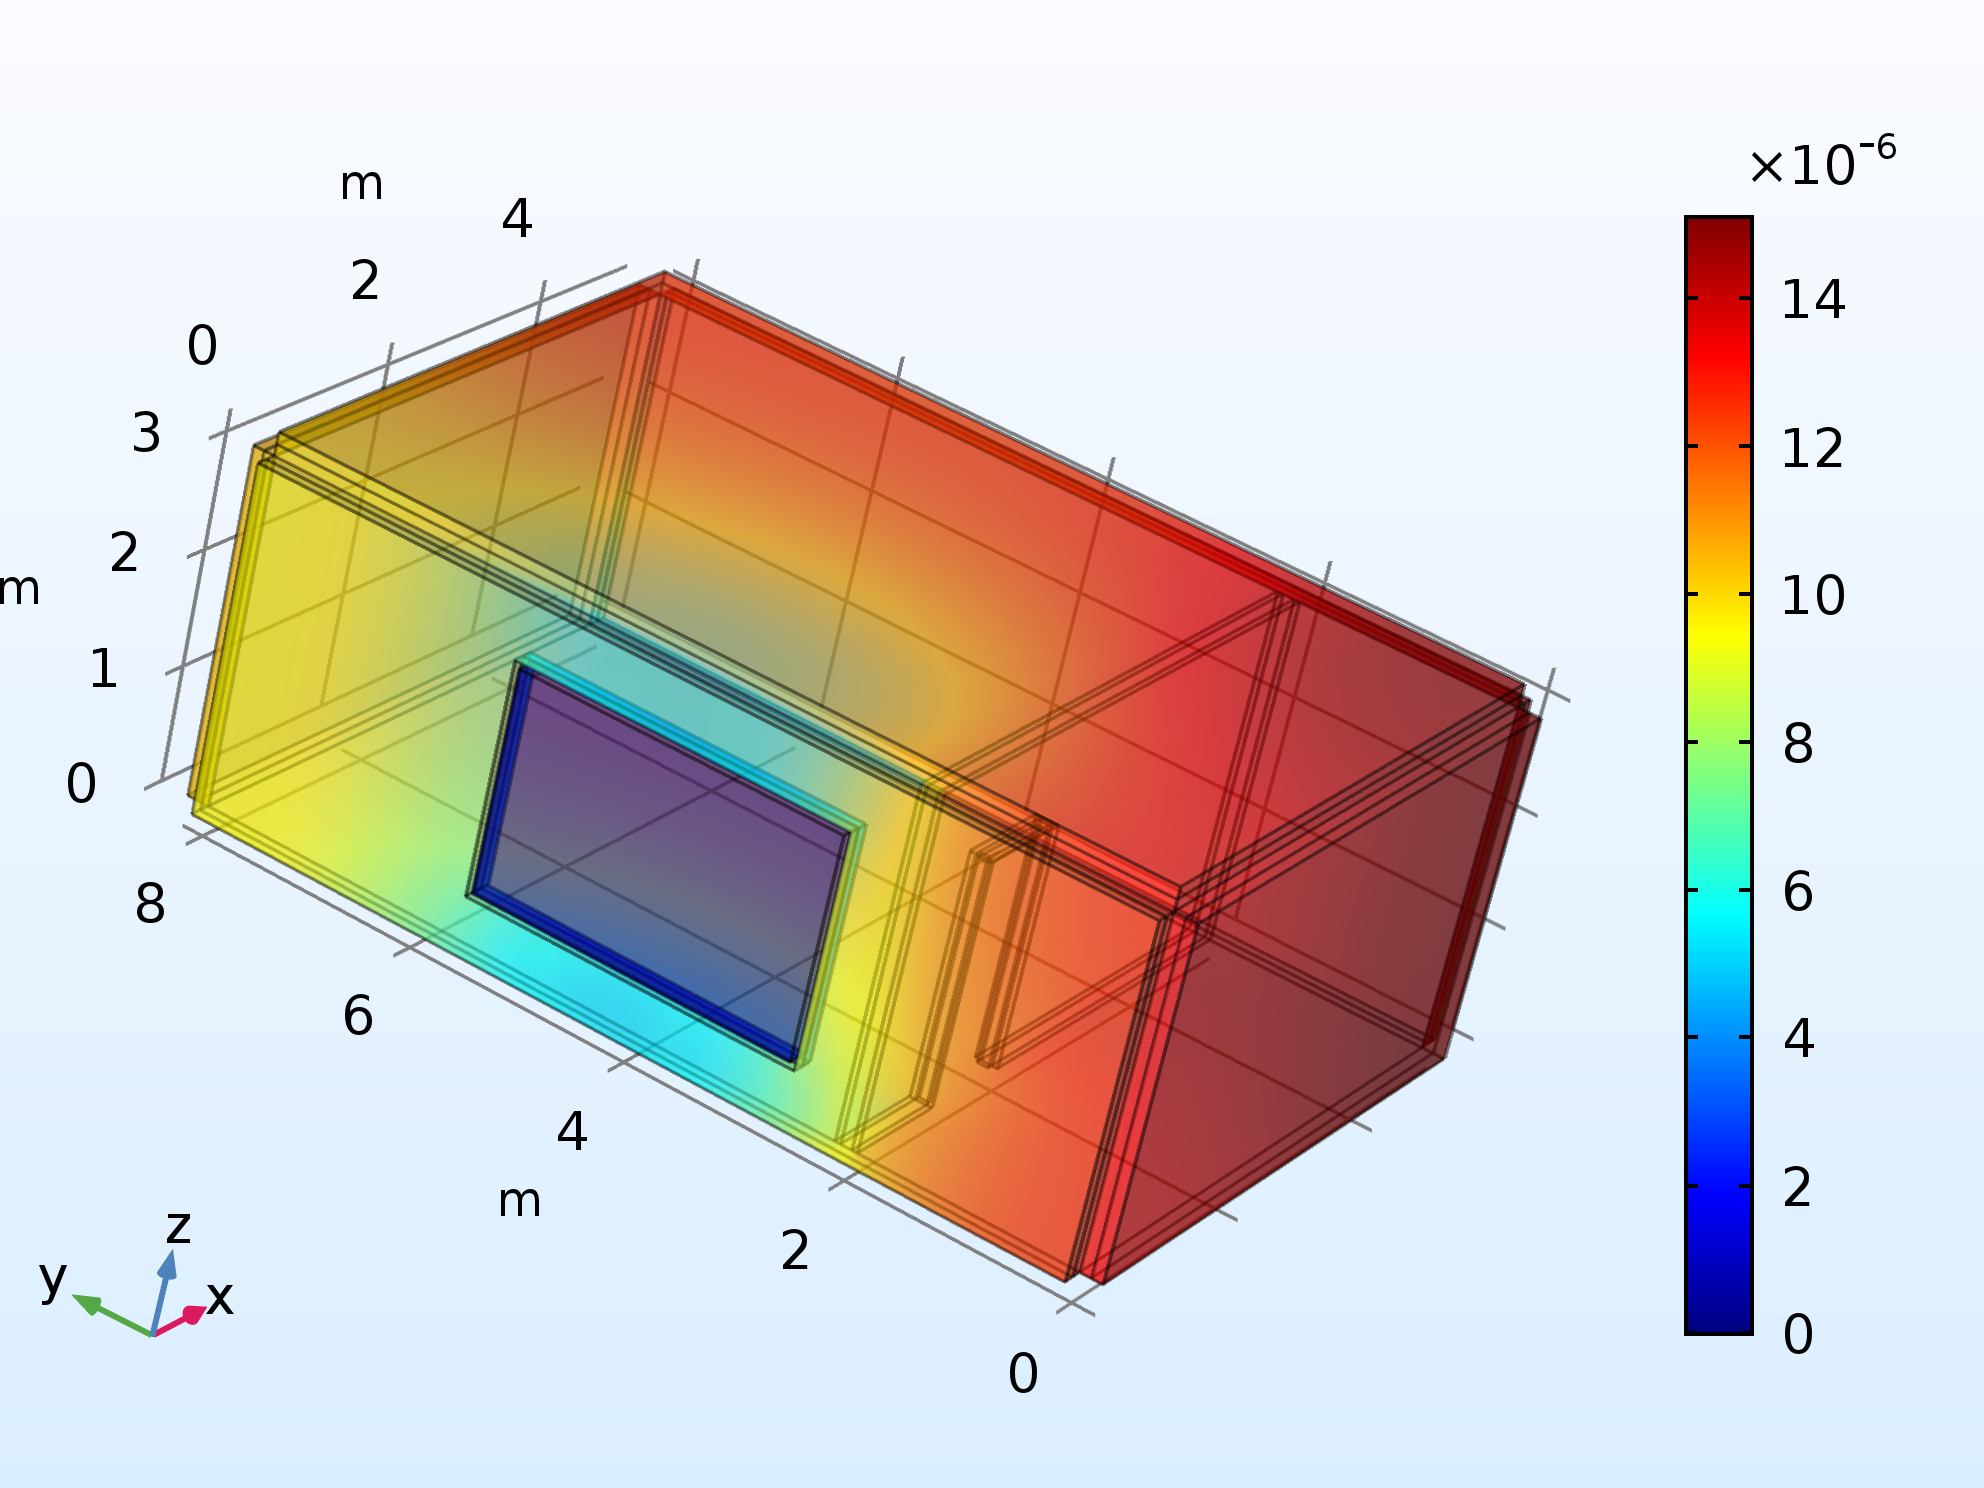
\includegraphics[width=\linewidth]{Month2.png}
    \caption{$M$=2}
  \end{subfigure}\\
  \begin{subfigure}[b]{0.3\linewidth}
    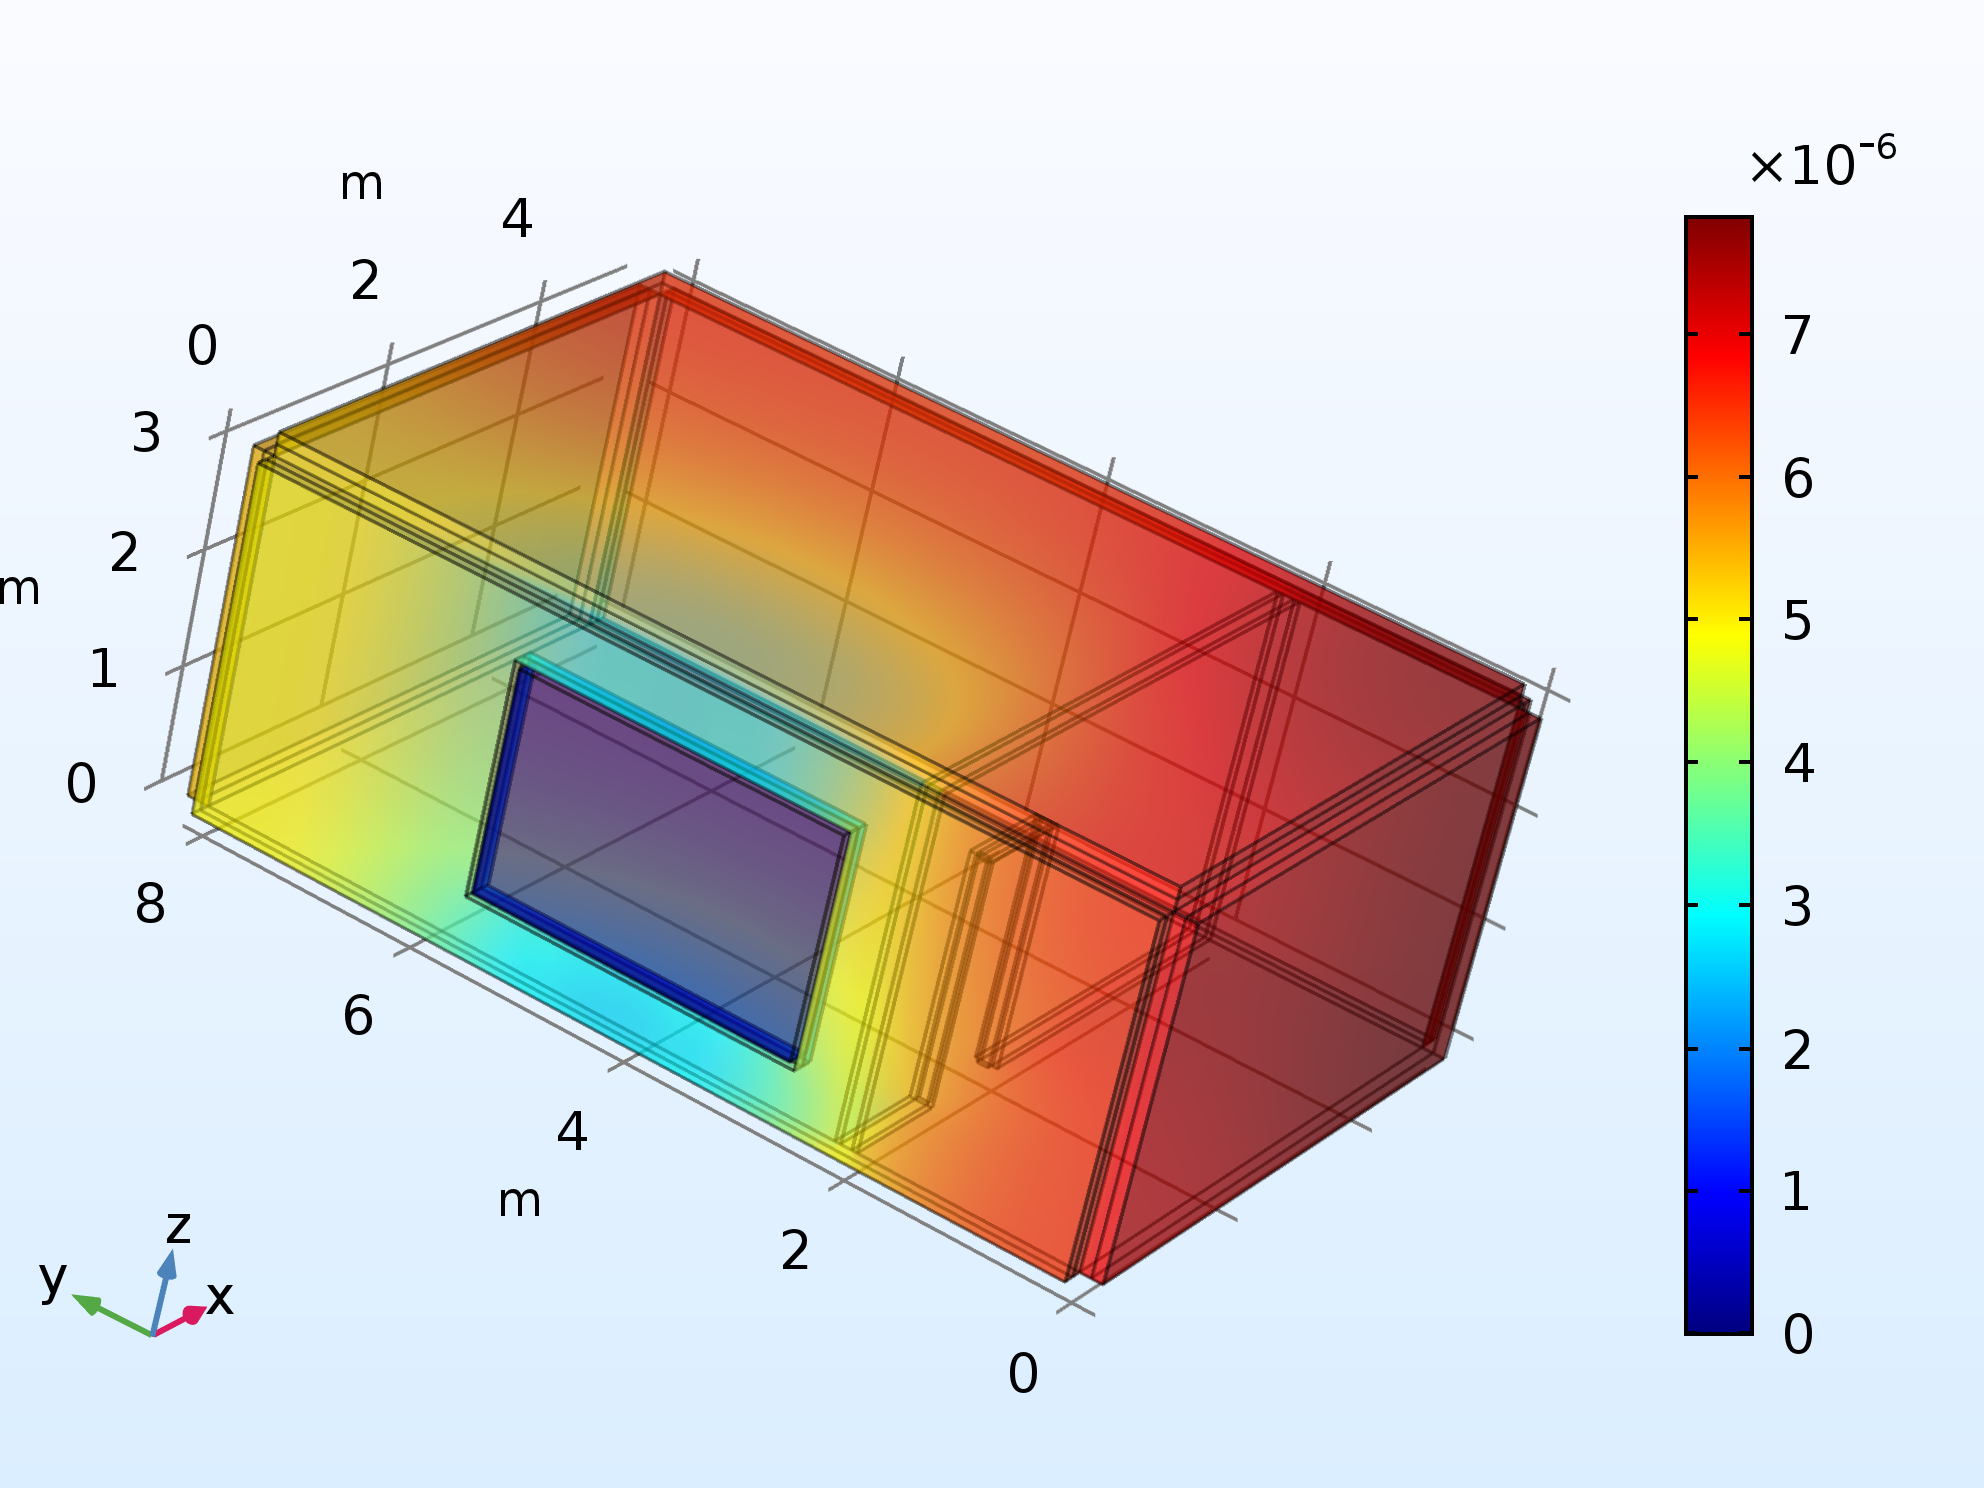
\includegraphics[width=\linewidth]{Month3.png}
    \caption{$M$=3}
  \end{subfigure}
  \begin{subfigure}[b]{0.3\linewidth}
    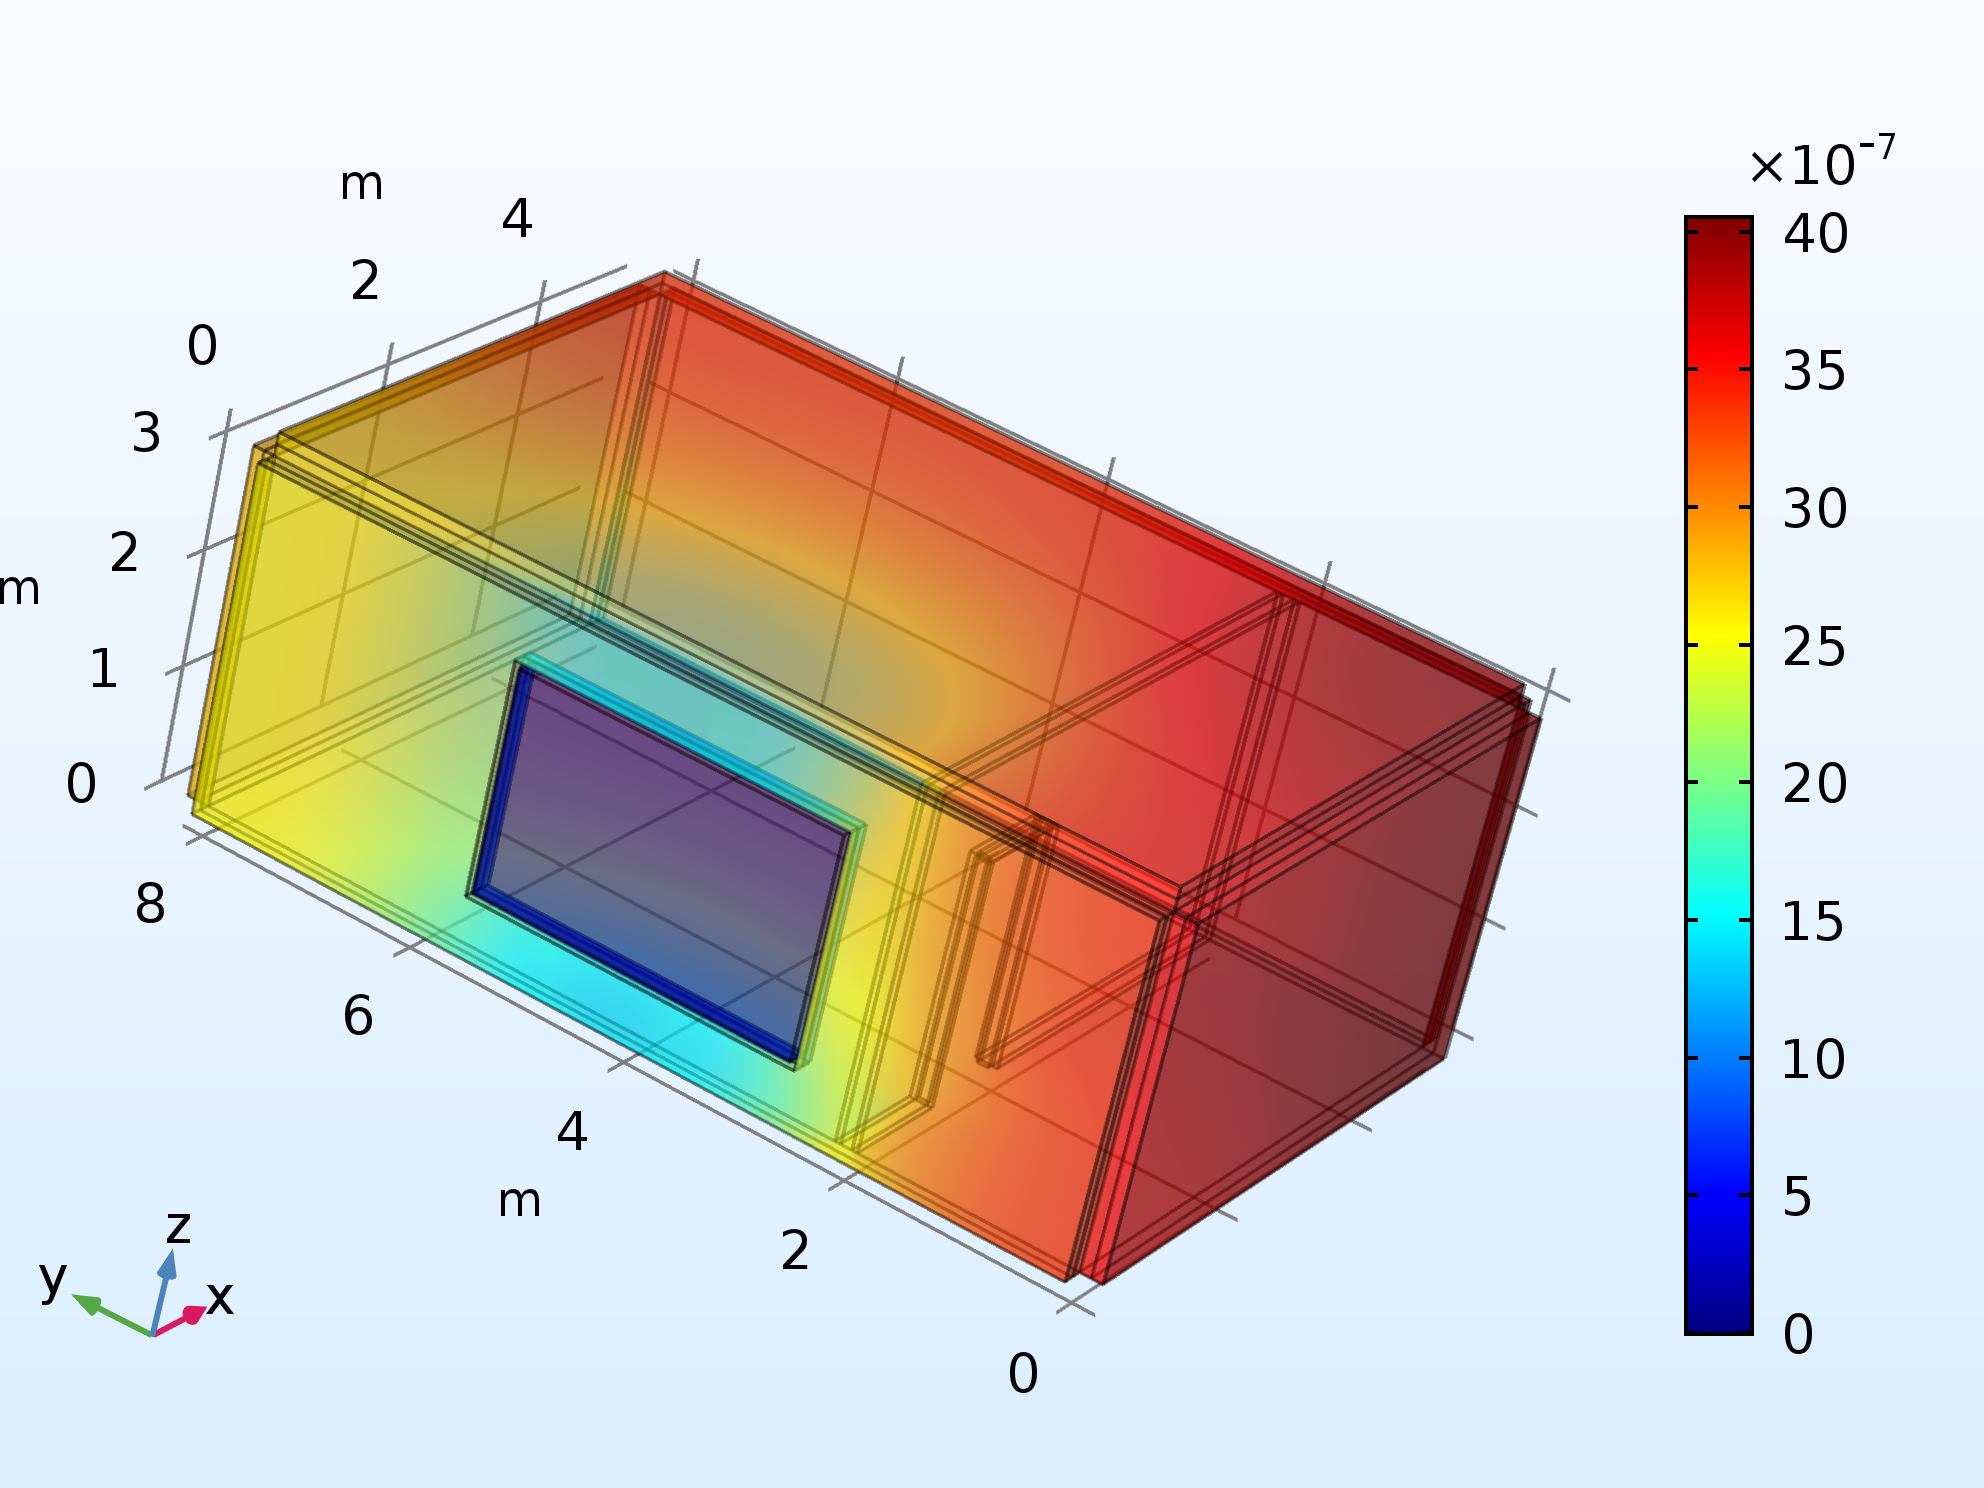
\includegraphics[width=\linewidth]{Month4.png}
    \caption{$M$=4}
  \end{subfigure}
  \begin{subfigure}[b]{0.3\linewidth}
    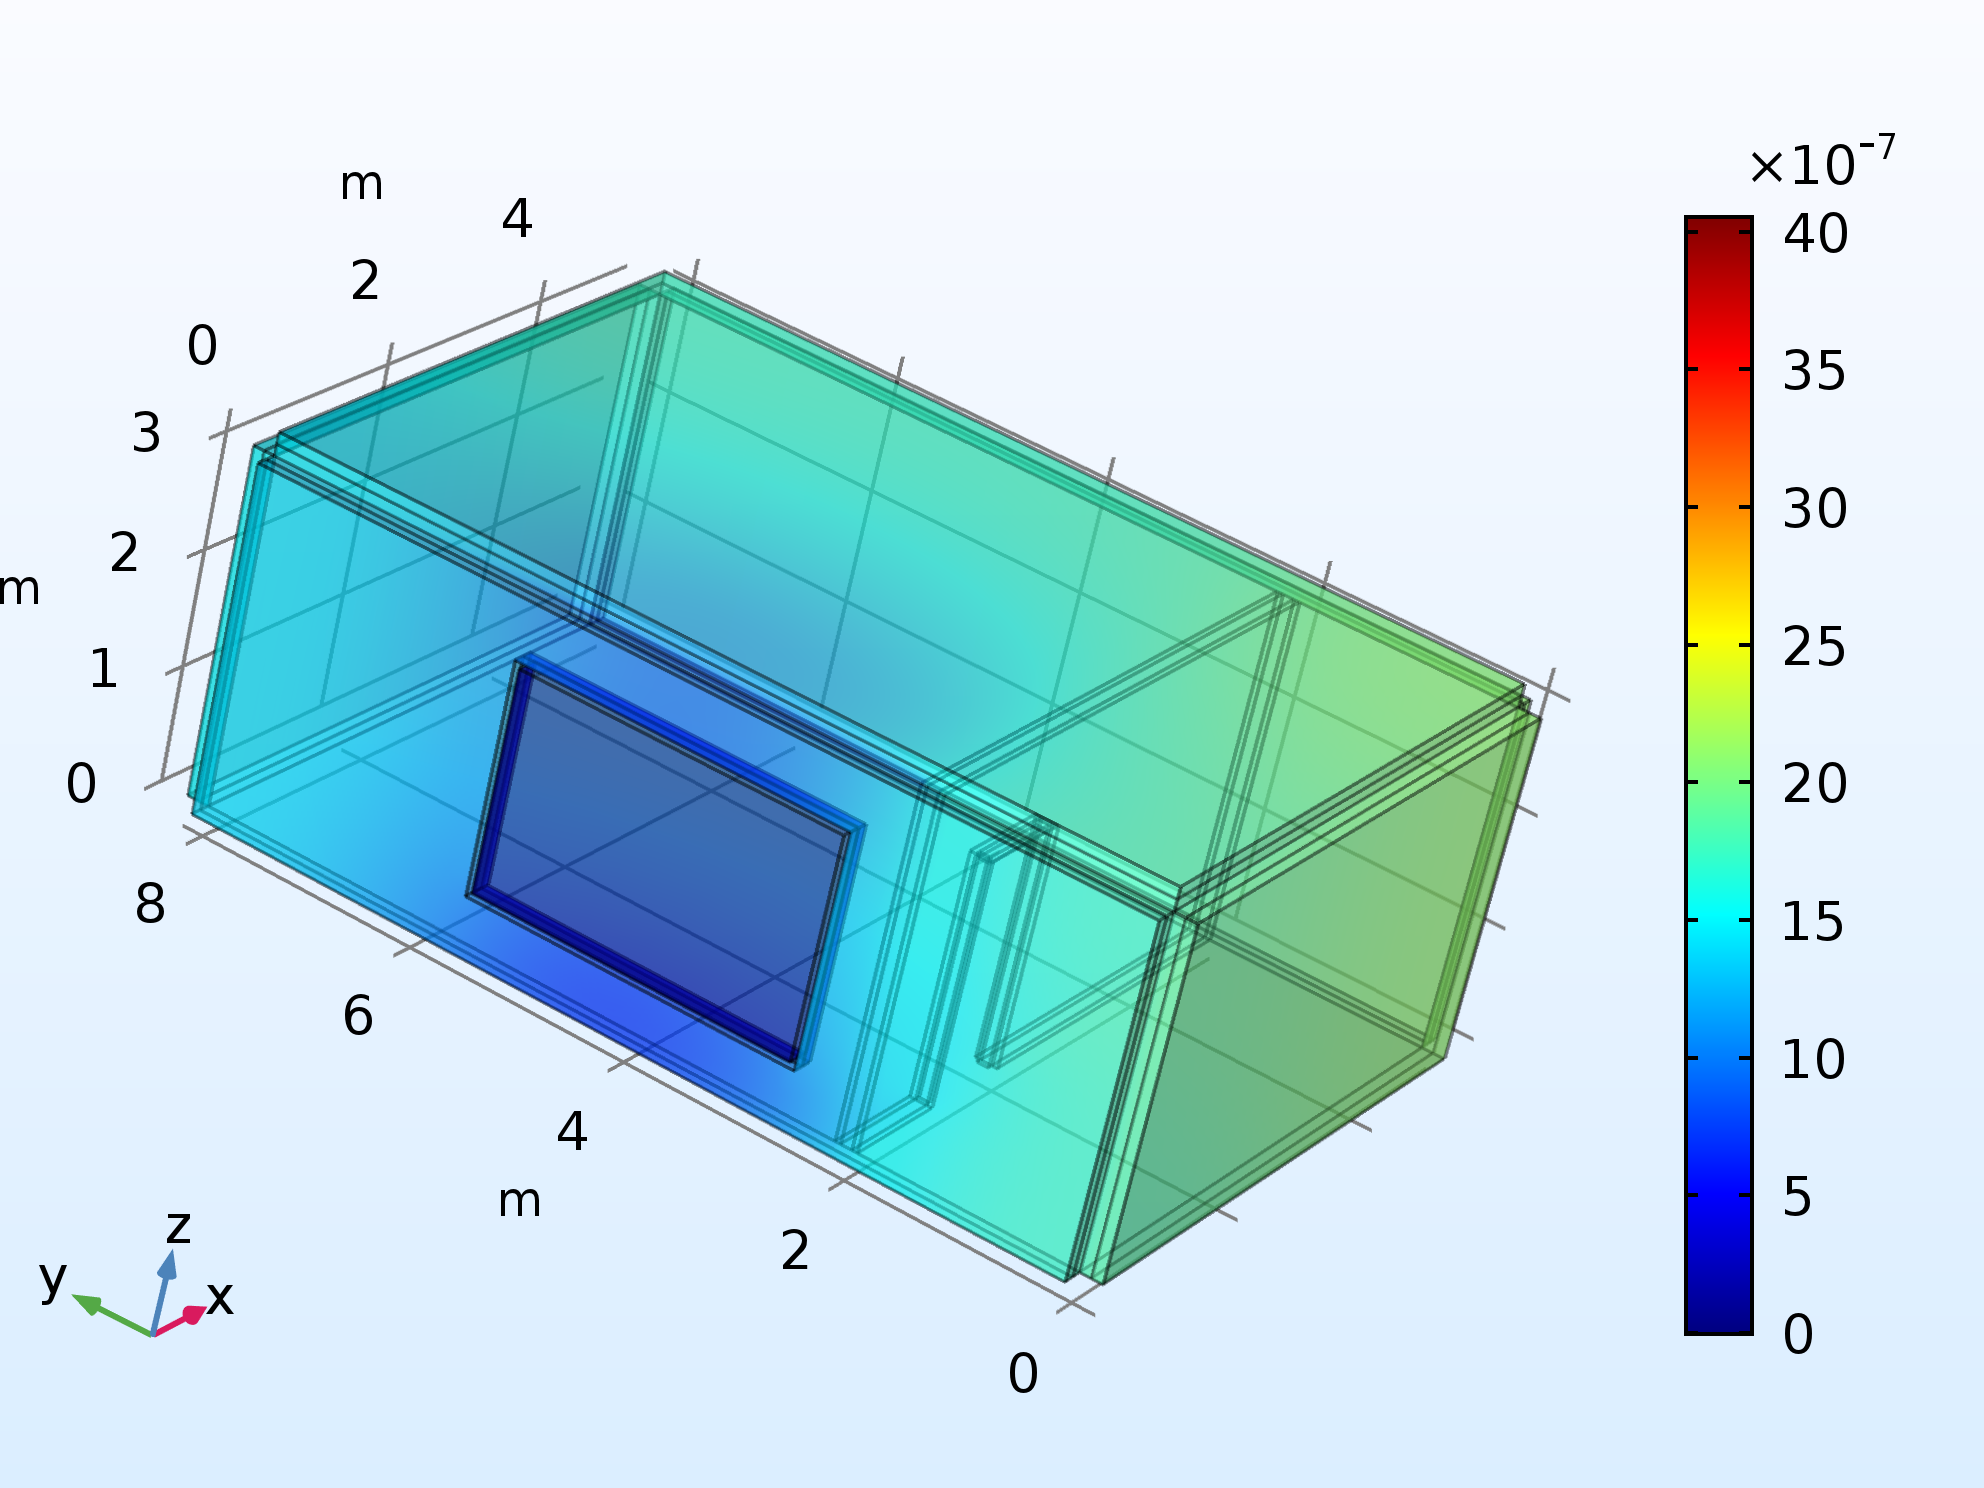
\includegraphics[width=\linewidth]{Month5.png}
    \caption{$M$=5}
  \end{subfigure}
  \caption{Simulation of the inner structure: interior walls}
  \label{fig:wall}
\end{figure}


From the figure above we can see that interior wall also bring inhomogeneous distribution just like the additional interior emission sources. What's more, the data derived from the simulation shows that it will take more time for the density of formaldehyde to decline, mainly because the wall will block the spread of formaldehyde.

\subsection{Strengths and Weakness}

\subsubsection{Strengths}
\begin{itemize}
\item We introduce three distinct models covering both discrete and continuous : LGA, MD, CF. After carefully analysis and evaluation we choose the most appropriate model to continue our work.
\item Our sensitivity analysis shows that our models are fairly robust to changes in parameter value so it can apply to many different situation in reality.
\item The assumptions in our models are reasonable, which can not only simplify the problems, but lay the foundation for the establishment of the latter model as well. 
\item In each model we discuss, we provide clear
and understandable graph to visualize the result of our model analysis.
\end{itemize}
 
\subsubsection{Weakness}
\begin{itemize}

\item In LGA model our simulation focus on 2D as it's hard to visualize the results in 3D.
\item In the strategy selection part we lack the detailed discussion over the trade-off between effect and energy cost.
 \end{itemize}

\section{Conclusions}

Our paper provides a detailed analysis of how the formaldehyde was emit and diffused, what strategies can we adopt to tackle with the formaldehyde hazard. Before introducing the model, we discussed the theory of diffusion. Then our models are proposed, made up of three distinct model: Lattice Gas Automata(LGA) model, Molecular Dynamic(MD) model and Continuous Fluid(CF) model. We use real data to simulate the emission and spread of formaldehyde.  

We have discovered that the CF model works well and have the best accuracy. Based on CF model, Different selective Strategies are fully discussed. Balance between effectiveness and energy-cost have been taken into consideration. Finally we put forward the composite strategy of combining window-opening with other effective strategy such as exhausting fans to adopt in the first few days, filling room with formaldehyde-absorbing plants. When different strategies are adopted, the time needed to decline to the health threshold are given: it takes over 106 days to decline to threshold by opening windows while it takes only 21 days when using exhausting fans.

\bibliographystyle{IEEEtran}
\bibliography{newrefs}

\newpage
\section*{Letter}
\addcontentsline{toc}{section}{Letter}

%%\begin{wrapfigure}{r}{7cm}%靠文字内容的左侧
%%
\includegraphics[width=7cm]{paint-cans-HHV.jpg}
%%\end{wrapfigure}


Dear local residents,

In the last few years, many of you have redecorated your houses by painting walls and replenishing rooms with some new furniture. It is universally acknowledged that paint and pressed-wood furniture emit formaldehyde. However, not all people attach much significance to its hazards: it can cause watery eyes in short terms while trigger cancer in long terms. Owing to these facts, we are writing this letter to offer you some simple advice to minimize the hazards.

We have been recently worked on the problem dealing with speeding up the emission of formaldehyde. We set up three models and proved that they are reliable by comparing their results to the actual circumstances. By modelling the exhaling of formaldehyde, we figured out that the best method to present the diffusion of the model is Continuous Fluid model, and our work on taking different strategies is based on that model. 

First of all, opening your windows as often as possible is definitely an easy approach you can take. By letting in sweet freeze, it can take away the contamination without consuming any energy. Our model has proved that by opening a window in a relatively small apartment for three months can ensure the concentration of formaldehyde meet the healthy threshold. If your room is larger, additional time is needed for the density to come to the safety threshold.

Secondly, you can install some exhausting fans. These would cost you some money, but the effect is prominent especially in the first three days. It can shorten the process of formaldehyde diffusion to only ten days. So, if you are in bad need to move into a newly painted room, you may consider this advice.

Thirdly, keeping the temperature and humidity in your house at a certain level also helps to speed up the diffusion. In our simulating experiments, temperature and humidity are in positive correlation with the diffusion of the formaldehyde. Therefore, keep in mind that the temperature in the room shouldn't be too high, and is suggested to be approximately 21 Celsius degrees. The best humidity is 50\%, which can be controlled by dehumidifiers and air-conditioners.

In a nutshell, if you have just renovated your house, you can try our advice. In this case, you are bound to get rid of the formaldehyde much faster. We sincerely hope that those simple approaches can make your life healthier and merrier.

\begin{flushright}
Best regards,
                                     
Team 73052
\end{flushright}
	
\newpage

\begin{appendices}

\section{Implemented LGA Model}
\lstinputlisting[language=C++]{codes/cell.h}
\lstinputlisting[language=C++]{codes/cell.cpp}
\lstinputlisting[language=C++]{codes/main.cpp}

\end{appendices}
\end{document}

%%
%% This work consists of these files mcmthesis.dtx,
%%                                   figures/ and
%%                                   code/,
%% and the derived files             mcmthesis.cls,
%%                                   mcmthesis-demo.tex,
%%                                   README,
%%                                   LICENSE,
%%                                   mcmthesis.pdf and
%%                                   mcmthesis-demo.pdf.
%%
%% End of file `mcmthesis-demo.tex'.
